
\documentclass[12pt,a4paper]{article}
%-------------------------------------------
%---Packages--------------------------------
%-------------------------------------------
\usepackage[utf8]{inputenc}
%\usepackage[T1]{fontenc}
%\usepackage{txfonts}
\usepackage{amsmath}
\usepackage{amsthm}
\usepackage{amsfonts}
\usepackage{array}
\usepackage{amssymb}
\usepackage{blindtext}
\usepackage{caption}
\usepackage{color}
\usepackage{csquotes}	    %
\usepackage{enumitem}	    %pour mieux bosser avec les listes. ajoute option label
\usepackage[yyyymmdd]{datetime}        %pour définir date custom
\usepackage{etaremune}
\usepackage{environ}
\usepackage{fancybox}
\usepackage{fancyhdr} 	    % Custom headers and footers
\usepackage{fancyref}
%\usepackage{float}
\usepackage{floatrow}       %float and floatrow can't be together...
\usepackage{gensymb}
\usepackage{graphicx}
\usepackage[colorlinks=true, linkcolor=purple, citecolor=cyan]{hyperref}
\usepackage{footnotebackref}
\usepackage{lipsum}
\usepackage{mathtools}
\usepackage{multicol}	    %gérer plusieurs colonnes
\usepackage{setspace}
\usepackage{subcaption}
\usepackage{todonotes}	    %Bonne gestion des TODOs
%TODO commenté pour tester l'utilité... à voir% \usepackage[tc]{titlepic}      %Permet de mettre une image en page de garde
\usepackage{tikz}	    % Pour outil de dessin puissant
\usepackage{ulem}	    %underline sur plusieurs lignes (avec \uline{})
\usepackage{vmargin} 	    %gestion des marges, avec dans l'ordre : gauche, haut, droit, bas, en-tête, entre en-tête et texte, bas de page, hauteur entre bas de page et texte
\usepackage{wrapfig}
\usepackage{xcolor}
\usepackage{xparse}                    %Pour utiliser NewDocumentCommand et des arguments 'mmooo'
%\usepackage{fullpage} 	    %supprime toutes les marges allouées aux notes, aussi en haut et en bas

%\ExplSyntaxOn
\pagestyle{fancyplain}	    %Makes all pages in the document conform to the custom headers and footers

%-------------------------------------------
%---Document Commands-----------------------
%---------------------------{----------------
\NewDocumentCommand{\framecolorbox}{oommm}
 {% #1 = width (optional)
  % #2 = inner alignment (optional)
  % #3 = frame color
  % #4 = background color
  % #5 = text
  \IfValueTF{#1}%
   {\IfValueTF{#2}%
    {\fcolorbox{#3}{#4}{\makebox[#1][#2]{#5}}}%
    {\fcolorbox{#3}{#4}{\makebox[#1]{#5}}}%
   }%
   {\fcolorbox{#3}{#4}{#5}}%
 }%
%------------------------------------------------
%------------------ENGLISH----------------------
%----------------------------------------------

\NewDocumentCommand{\epflTitle}{mO{Olivier Cloux}O{\today}O{Notes de Cours en}D<>{../../Common}}%Arguments : Matière, Auteur, Date, Titre du doc
{
\begin{titlepage}
    \vspace*{\fill}
    \begin{center}
        \normalfont \normalsize
        \textsc{Ecole Polytechnique Fédérale de Lausanne} \\ [25pt] % Your university, school and/or department name(s)
        \textsc{#4} %Titre du doc
        \\ [0.4 pt]
        \horrule{0.5pt} \\[0.4cm] % Thin top horizontal rule
        \huge #1 \\ % Matière
        \horrule{2pt} \\[0.5cm] % Thick bottom horizontal rule
        
\includegraphics[width=8cm]{#5/EPFL_logo}
        ~\\[0.5 cm]
        \small\textsc{#2}\\[0.4cm]
        \small\textsc{#3}\\
        ~\\
        ~\\
        
\includegraphics[scale=0.5]{#5/creativeCommons}
    \end{center}
    \vspace*{\fill}
\end{titlepage}
}


%-------------------------------------------
%-------------MATH NEW COMMANDS-------------
%-------------------------------------------
\newcommand{\somme}[2]{\ensuremath{\sum\limits_{#2}^{#1}}}
\newcommand{\produit}[2]{\ensuremath{\prod\limits_{#2}^{#1}}}
\newcommand{\limite}{\lim\limits_}
\newcommand{\llimite}[3]{\limite{\substack{#1 \\ #2}}\left(#3\right)}	%limites à deux condiitons
\newcommand{\et}{\mbox{ et }}
\newcommand{\deriv}[1]{\ensuremath{\, \mathrm d #1}}	%sigle dx, dt,dy... des dérivées/intégrales
%\newcommand{\fx}{\ensuremath{f'(\textbf{x}_0 + h}}
\newcommand{\ninf}{\ensuremath{n \to \infty}}	       %pour les limites : n tend vers l'infini
\newcommand{\xinf}{\ensuremath{x \to \infty}}	       %pour les limites : x tend vers l'infini
\newcommand{\infint}{\ensuremath{\int_{-\infty}^{\infty}}}
\newcommand{\xo}{\ensuremath{x \to 0}}									%x to 0
\newcommand{\no}{\ensuremath{n \to 0}}									%n zéro
\newcommand{\xx}{\ensuremath{x \to x}}									%x to x
\newcommand{\Xo}{\ensuremath{x_0}}										%x zéro
\newcommand{\X}{\ensuremath{\mathbf{X}} }
\newcommand{\A}{\ensuremath{\mathbf{A}} }
\newcommand{\R}{\ensuremath{\mathbb{R}} }								%ensemble de R
\newcommand{\rn}{\ensuremath{\mathbb{R}^n} } 							%ensemble de R de taille n
\newcommand{\Rm}{\ensuremath{\mathbb{R}^m} }  							%ensemble de R de taille m
\newcommand{\C}{\ensuremath{\mathbb{C}} }
\newcommand{\N}{\ensuremath{\mathbb{N}} }
\newcommand{\Z}{\ensuremath{\mathbb{Z}} }
\newcommand{\Q}{\ensuremath{\mathbb{Q}} }
\newcommand{\rtor}{\ensuremath{\R \to \R} }
\newcommand{\pour}{\mbox{ pour }}
\newcommand{\coss}[1]{\ensuremath{\cos\(#1\)}}						%cosinus avec des parenthèses de bonne taille (genre frac)
\newcommand{\sinn}[1]{\ensuremath{\sin\(#1\)}}					%sinus avec des parentèses de bonne taille (genre frac)
\newcommand{\txtfrac}[2]{\ensuremath{\frac{\text{#1}}{\text{#2}}}}		%Fractions composées de texte
\newcommand{\evalfrac}[3]{\ensuremath{\left.\frac{#1}{#2}\right|_{#3}}}
\renewcommand{\(}{\left(}												%Parenthèse gauche de taille adaptive
\renewcommand{\)}{\right)}
\newcommand{\longeq}{=\joinrel=}												%Parenthèse droite de taille adaptive


%-------------------------------------------------------
%------------------MISC NEW COMMANDS--------------------
%-------------------------------------------------------
\newcommand{\degre}{\ensuremath{^\circ}}
%\newdateformat{\eudate}{\THEYEAR-\twodigit{\THEMONTH}-\twodigit{\THEDAY}}



%-------------------------------------------------------
%------------------TEXT NEW COMMANDS--------------------
%-------------------------------------------------------
\newcommand{\ts}{\textsuperscript}
\newcommand{\evid}[1]{\textbf{\uline{#1}}}        %mise en évidence (gras + souligné)



%\newcommand{\Exemple}{\underline{Exemple}}
\newcommand{\Theoreme}{\underline{Théorème}}
\newcommand{\Remarque}{\underline{Remarque}}
\newcommand{\Definition}{\underline{Définition} }
\newcommand{\skinf}{\sum^{\infty}_{k=0}}
\newcommand{\combi}[2]{\ensuremath{\begin{pmatrix} #1 \\ #2 \end{pmatrix}}}	%combinaison parmi 1 de 2
\newcommand{\intx}[3]{\ensuremath{\int_{#1}^{#2} #3 \deriv{x}}}				%intégrale dx
\newcommand{\intt}[3]{\ensuremath{\int_{#1}^{#2} #3 \deriv{t}}}				%intégrale dy
\newcommand{\misenforme}{\begin{center} Mis en forme jusqu'ici\\ \line(1,0){400}\\ normalement juste, mais à améliorer depuis ici\end{center}}	%raccourci pour mise en forme
\newcommand*\circled[1]{\tikz[baseline=(char.base)]{
            \node[shape=circle,draw,inner sep=1pt] (char) {#1};}}			%pour entourer un chiffre
\newcommand{\horrule}[1]{\rule{\linewidth}{#1}} 				% Create horizontal rule command with 1 argument of height

\theoremstyle{definition}
\newtheorem{exemp}{Exemple}
\newtheorem{examp}{Example}


%-------------------------------------------
%---Environments----------------------------
%-------------------------------------------
\NewEnviron{boite}[1][0.9]{%
	\begin{center}
		\framecolorbox{red}{white}{%
			\begin{minipage}{#1\textwidth}
 	 			\BODY
			\end{minipage}
		}
	\end{center}
}
\NewEnviron{blackbox}[1][0.9]{%
	\begin{center}
		\framecolorbox{black}{white}{%
			\begin{minipage}{#1\textwidth}
 	 			\BODY
			\end{minipage}
		}
	\end{center}
}
\NewEnviron{exemple}[1][0.8]{%
    \begin{center}
        \framecolorbox{white}{gray!20}{%
            \begin{minipage}{#1\textwidth}
                \begin{exemp}
                    \BODY
                \end{exemp}
            \end{minipage}
        }
    \end{center}
}
\NewEnviron{suiteExemple}[1][0.8]{%
    \begin{center}
        \framecolorbox{white}{gray!20}{%
            \begin{minipage}{#1\textwidth}
                \BODY
            \end{minipage}
        }
    \end{center}
}
\NewEnviron{colExemple}[1][0.8]{%
    \begin{center}
        \framecolorbox{white}{gray!20}{%
            \begin{minipage}{#1\columnwidth}
                \begin{exemp}
                    \BODY
                \end{exemp}
            \end{minipage}
        }
    \end{center}
}
\NewEnviron{example}[1][0.8]{%
    \begin{center}
        \framecolorbox{white}{gray!20}{%
            \begin{minipage}{#1\textwidth}
                \begin{examp}
                    \BODY
                \end{examp}
            \end{minipage}
	}
    \end{center}
}
\NewEnviron{systeq}[1][l]{
			\begin{center}
				$\left\{\begin{array}{#1}
					\BODY
				\end{array}\right.$
			\end{center}
 }





%-------------------------------------------
%---General settings-----------------------
%-------------------------------------------
\renewcommand{\headrulewidth}{1pt}										%ligne au haut de chaque page
\renewcommand{\footrulewidth}{1pt}										%ligne au pied de chaque page
\setstretch{1.6}
\author{Olivier Cloux}

\newcommand{\Exemple}{\underline{Exemple} }

\begin{document}
\epflTitle{Analyse I}[Olivier Cloux][Automne 2014][Notes de Cours en][../../../Common]
%\maketitle
\tableofcontents

\section{Rappels}
\subsection{Fonctions trigonométriques}
\begin{center}
\[\cos(x) = \sin(\frac{\pi}{2} + x)\]
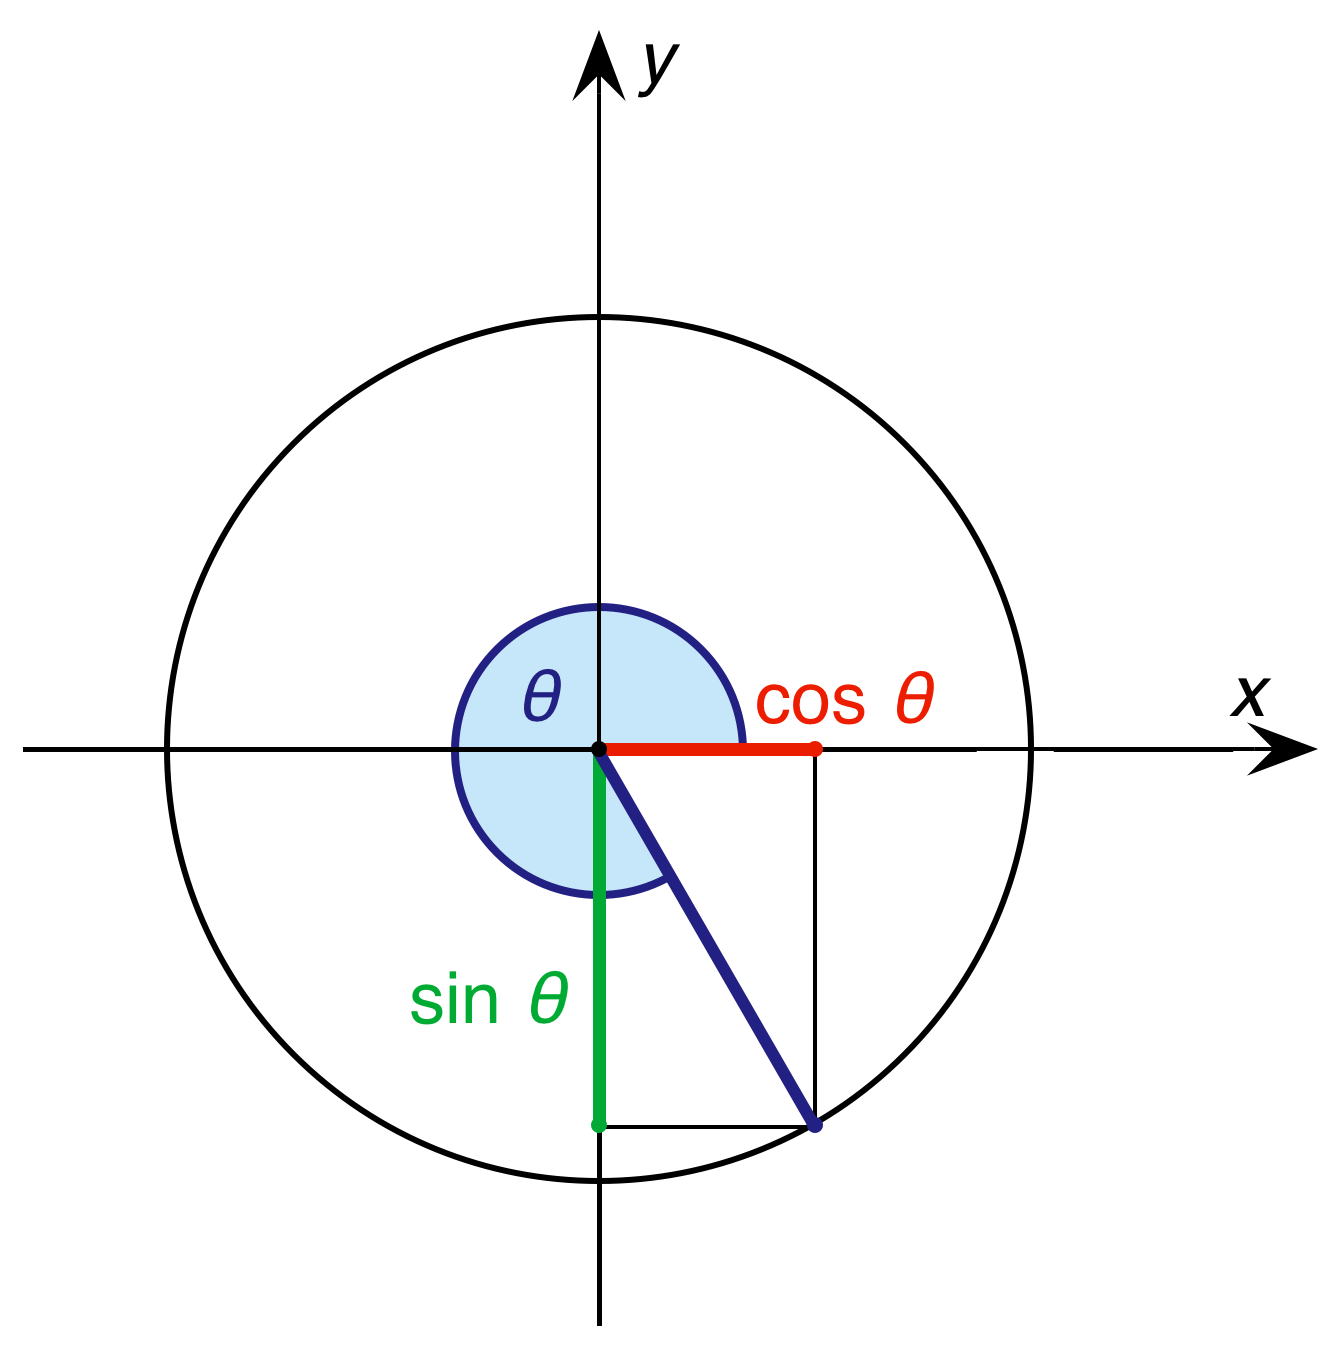
\includegraphics[scale=0.2]{illustrations_Analyse/sin_and_cos}
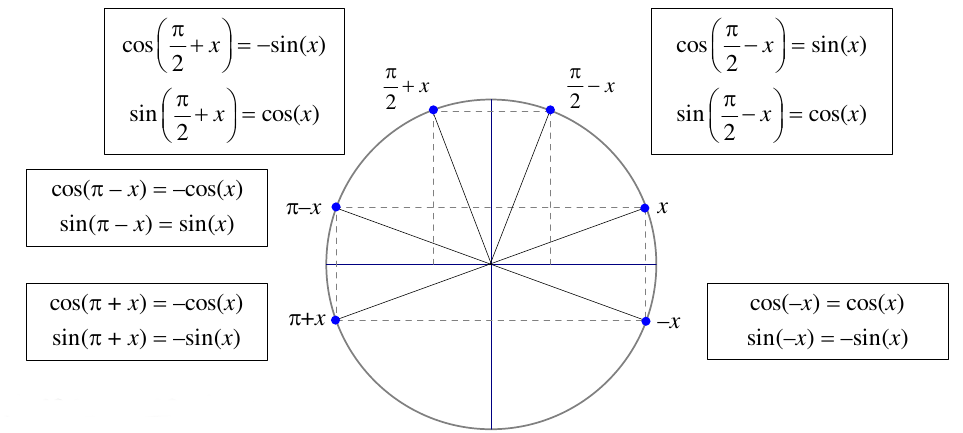
\includegraphics[scale=0.7]{illustrations_Analyse/trigo}\\
%\includegraphics[scale=0.8]{illustrations_Analyse/sin_and_cos2}
\end{center}
\subsection{Logarithme}
\begin{itemize}
	\item $\log_a(x) = y \iff x =  a^y,\forall$
	\item $a^{\log_a(x)} = x$
	\item $\log_a(a^x) = x\log_a(a) = x \cdot 1 = x$
	\item $log_a(1) = 0, log_a(a) = 1$
\end{itemize}

\subsection{Paires de fonctions réciproques}
Deux fonctions $f$ et $g$ sont réciproques si $f(g(x)) = g(f(x)) = x$\\
Par exemple :
\begin{itemize}
\item $x^2$ et $\sqrt{x}$ sont réciproques pour tout nombre $\geq 0$
\item $e^x = \exp(x)$ et $\ln(x) (e \simeq 2.71828)$ sont réciproques pour tout nombre positif.
\item $a^x$ et $\log(x)$
\item $\log_a(x\cdot y) = \log_a(x) + \log_a(y)$
\item $\log_a(\frac{1}{x}) = \log_a(x^{-1}) = -\log(x)$
\item $\log_a(\frac{x}{y}) = \log_a(x \cdot \frac{1}{y}) =\log_a(x) + \log_a(\frac{1}{y}) = \log_a(x) - \log_a(y)$
\item $\log_a(x^r) = r\cdot \log_a(x)$
\end{itemize}

\section{Chapitre 1 : Ensembles}
\setcounter{equation}{0}
\begin{center}
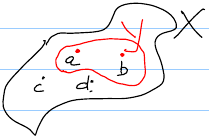
\includegraphics[scale=1]{illustrations_Analyse/ensemble}\\	
\end{center}
On peut définir $Y =\{x \in X :$ couleur(x) = rouge\}
\subsection{Notations}
\begin{center}
\begin{tabular}{lll}
$\in $&  est élément de & $a \in y$\\
$\not \in $& n'est pas élément de &$ c \notin y$\\
$\subset $ &  est un sous-ensemble & $y \subset y$\\
$\not \subset$ & n'est pas un sous-ensemble & $x \not\subset y$\\
$=$ & est le même ensemble que & y = y\\
$\neq$ &  n'est pas le même ensemble que & $x \neq y$\\
$\emptyset$ & ensemble vide, ensemble sans élément\\
\end{tabular}
\end{center}
\textbf{Nota bene :}
\begin{itemize}[label=\textbullet,itemsep=-10pt]
\item $\emptyset \subset x \forall x$
\item $x \subset x$
\item $\{a,b\} = \{b,a\}$, mais $\{a,b\} \neq \{\{a\},\{b\}\}\}$
\item $| \mathbf{X}|$ Cardinalité d'un ensemble. $\mathbf{X} = \{a, b, c, d\} \to |\mathbf{X}| = 4$
\item $P(\mathbf{X})$ l'ensemble de tous les sous-ensembles de X. Il vaut $2^{|\mathbf{X}|} = 2^4 = 16$ sous-ensembles.
\end{itemize}

\subsubsection{Le produit cartésien}
$\mathbf{X}, \mathbf{Y}$ des ensembles. $\mathbf{X} \times \mathbf{Y} := \{(x,y) : x \in \mathbf{X}, y \in \mathbf{Y}\}$
\\\underline{Exemple :} X = \{1,2\}, Y = \{3,4\}. $\mathbf{X} \times \mathbf{Y} = \{(1,3), (2,3), (1,4) (2,4)\}$

\subsubsection{Classes d'équivalence}
On peut vouloir décomposer un ensemble $\mathbf{X}$ en classes d'équivalences.
\\\underline{Remarque :} Le symbole $\sim$ définit une relation d'équivalence\newline
3 relations d'équivalence sur X : 

\begin{itemize}
\item[Réflexive] $x \sim x, \forall x \in \mathbf{X}$
\item[Symétrique] x $\sim$ y $\Rightarrow$ y $\sim$ x
\item[Transitive] x $\sim$ y, y $\sim$ z $\Rightarrow$ x $\sim$ z
\end{itemize}
\begin{boite}
\underline{Définition :} $C_x := \{y \in \mathbf{X} : \sim x\} \equiv [x]$\\
$C_x \in \mathbf{X}$ la classe d'équivalence de x
\end{boite}

\begin{boite}
\underline{Définition :} L'ensemble quotient $\mathbf{X}/ \sim$ est l'ensemble des classes d'équivalences distinctes de X
\end{boite}
\evid{Terminologie :} Soit C $\in$ X/$\sim$ alors x $\in$ C est appelé un représentant de C


\subsubsection{Fonctions, applications}
\begin{itemize}
\item[\textbf{Surjection}] Tout point de $\mathbf{Y}$ est atteint par au moins un x, soir si \underline{Im(f) = Y}
\item[\textbf{Injection}] Tous les points de $\mathbf{X}$ ont un et un seul y. $\mathbf{Y}$ peut avoir des points "vides" $\to$ \underline{$f(x_1) = f(x_2) \to x_1 = x_2$}
\item[\textbf{Bijection}] Chaque point de X et de Y a une et une seule réciproque
\end{itemize}
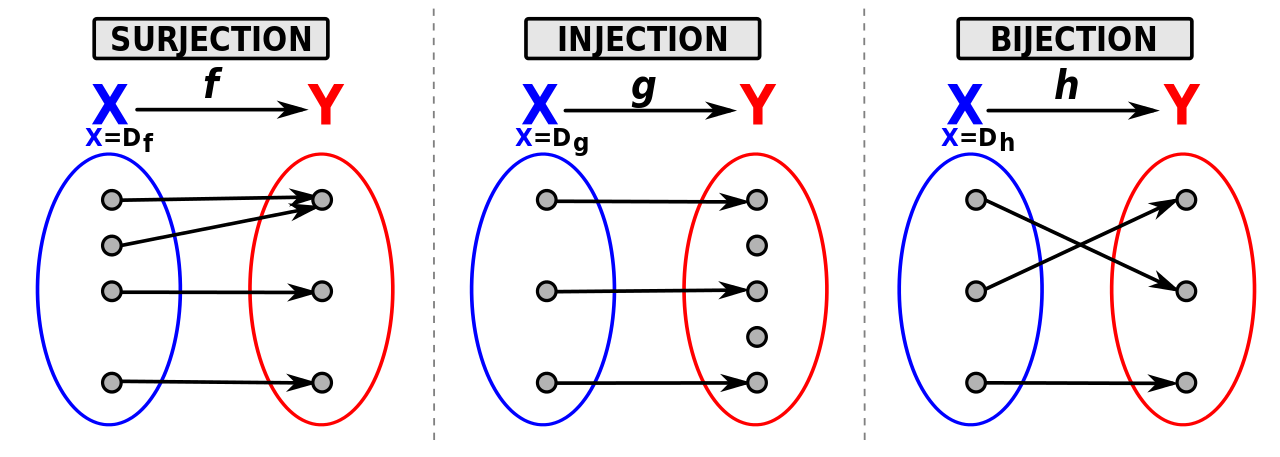
\includegraphics[scale=0.35]{illustrations_Analyse/fonctions}\\
\evid{Domaine de définition de f:}\\
$\mathbf{D} \equiv \mathbf{D}_f \equiv \mathbf{D}(f) := \{x \in \mathbf{X}$ : une flèche (et une seule) va de $x \in \mathbf{X}$ vers un $y \in \mathbf{Y}$\}\\
Si $\mathbf{D} = \mathbf{X}$, on parle aussi d'une application\\
\\
\evid{Image de f :} $Im(f) \equiv f(\mathbf{D}) := \{y \in \mathbf{Y} : y = f(x)$ pour un $x \in \mathbf{D}$\}\\
\underline{Remarque:} Toute fonction $f: \mathbf{D} \to $ Y définit une fonction surjective si on remplace Y par Im(f) $<$ y
\begin{boite}\Definition : Une fonction qui est injective et surjective est appelée bijective.
\end{boite}
\underline{Remarque :} Toute fonction $f : \mathbf{D} \to \mathbf{Y}$ qui est injective définit une fonction bijective de $\mathbf{D} \to Im(f)$.

\subsubsection{Notation et terminologie}
\begin{enumerate}%[label=\roman*]
\item Donné g. h = g$|_{\mathbf{D}_h}$. = "h est égal à g restreint à $\mathbf{D}_h \subset \mathbf{D}_g$ ou h est une restriction de g.
\item Donné h : g$\|_{\mathbf{D}_h}$ = h = g est un prolongement de h.
\end{enumerate}

\subsubsection{Le graphe d'une fonction f}
\begin{boite}
\Definition : Le graphe d'une fonction f : $\mathbf{\mathbf{D}} \to \mathbf{Y}$ est l'ensemble $G_f = \equiv G(f) := \{ (x,y) \in \mathbf{\mathbf{D}} \times \mathbf{Y} : y = f(x)\}$
\end{boite}

\subsubsection{Définition d'une fonction par son graphe}
Soit $G \subset \mathbf{\mathbf{D}} \times \mathbf{Y}$ tel que pour tout $x \in \mathbf{D}$, alors il existe un y et un seul tel que $(x,y) \in G$. Alors G est le graphe d'une fonction (application) f : $\mathbf{D} \to Y$, qui pour $(x,y) \in G$ associe y à x
\subsubsection{Composition de fonction}
\begin{equation}
h = f \circ g
\end{equation}
Soit\begin{equation}
\mathbf{D} := \{x \in \mathbf{D}_f : y = f(x) \in \mathbf{D}_g\} \subset \mathbf{D}_f
\end{equation} 
Alors on peut définir la fonction $h : \mathbf{D} \to Z$ par $h(x) := g(f(x))$.
\evid{Notation} on écrit  $h = g \circ f$ pour une fonction définie ainsi. On dit que h est la composition de g avec f, ou que h est ``g rond f''
\subsubsection{Compositions multiples}
\begin{equation}
(h \circ g) \circ f = h\circ (g \circ f) = h \circ g \circ f
\end{equation}
La loi de composition de fonctions est associative
\subsubsection{Fonction réciproque}
Soit $f: \mathbf{X} \to \mathbf{Y}$ avec $D_f = x$ une fonction bijective. Alors on peut définir une fonction dite \textit{réciproque}
g(f(x)) = x , x $\in$ X\\
f(g(y)) = y , y $\in$ Y\\
ou g $\circ$ f = Id (identité)\\
f $\circ$ g = Id.\\
\begin{boite}
\Definition : Soit f : $\mathbf{X} \to \mathbf{Y}$ avec $\mathbf{D}_f = X$ une fonction bijective. Alors on peut définir une fonction dite réciproque $g\equiv f^{-1} : Y \to X$. par : g(y) = x   où x est l'unique solution de l'équation f(x) = y. On a $\mathbf{D}_{f^{-1}} = Y$et $f^{-1}$ est bijective
\end{boite}

\subsection{Les entiers ($\N, \Z$)}
Les entiers naturels \\
$\begin{array}{ll}
\N = \{0, 1, 2, 3,...\}\\
\N* = \{1,2,3,...\} & = \N \mbox{ privé de } 0 \\
&= \N\setminus \{0\}
\end{array}$\\
\evid{Nota bene} : 0 est un nombre pair.

\subsubsection{Relation d'ordre (totale) $\leq$}
Pour tout $x, y, z \in \N$
\begin{enumerate}
\item $x \leq y \et y \leq z \Rightarrow x \leq z$
\item $x \leq y \et y \leq x \Rightarrow x = y$
\item on a soit $x \leq y \mbox{ soit } y \leq x$ (ordre totale)
\end{enumerate}
\evid{Notation :} on écrit $x<y$ si $x \leq y$ et $x \neq y$, $x \geq y$ si $y \leq x$, $x > y$ si $y < x$
\underline{Remarque :} $\Leftrightarrow$ 3' : on a soit $x < y$, soit $x = y$, soit $x > y$\\
\evid{Propriété de bon ordre :} Tout sous-ensemble non-vide X de $\N$ a un plus petit élément, CàD :
\begin{equation}
\forall X \subset \N, \exists x \in X \mbox{ tel que }x \leq y\mbox{ pour tout }y \in X
\end{equation}
\underline{Exemple :} X = \{1,2,3\} , x = 1, le plus petit élément car pour tout $x \in X$, on a $1 \leq x$

\subsubsection{Opérations :}
\begin{itemize}
\item[\textbf{+}] $\underset{(m,n)}{\N \times \N} \underset{\to}{\to} \underset{(m+n)}{\N}$	 
\item[\textbf{$\cdot$}] $\underset{(m,n)}{\N \times \N} \underset{\to}{\to} \underset{(m\cdot n)}{\N}$	 
\end{itemize}
\subsubsection{Élément neutre}
\begin{itemize}
\item 0 pour l'addition : $n+0 = n \forall n \in \N$
\item 1 pour la multiplication : $n \cdot 1 = n \forall n \in \N$
\end{itemize}
On n'a pas encore (sur \N)d'élément "inverse" pour l'addition et la multiplication.

\subsubsection{Compatibilité de $\leq$ avec + et $\cdot$}
\begin{enumerate}%[label=\roman*]
\item Si $x \leq y$ alors $x+z \leq y + z \forall z \in \N$
\item Si $ 0 \leq x$ et $0 \leq y$ alors $0 \leq x \cdot y$ 
\end{enumerate}

\subsubsection{Les entiers (relatifs)}
$\mathbb{Z} = \{-2, -1, 0, 1, 2, 3,...\}$\\
$\mathbb{Z*}$ = $\Z \setminus \{0\}$ = le même sans le 0.\\
\evid{Élément inverse pour +} Pour tout $x \in \Z$ il existe $y \in \Z$ tel que x+y = 0\\
\evid{Notation :} on écrit 2 -3 au lieu de 2 + (-3) car -(-3) = 3

\subsubsection{PGDC}
Algorithme d'Euclide, Algorithme de Joseph Stein.\\
\evid{Remarque de base :} Soit $0 \leq b \leq a$. Si r divise a et si r divise b, alors r divise a-b.\\
\underline{Algorithme de Stein}
\begin{enumerate}
\item pgdc(a,b) = pgdc(b,a).
\item pgdc(a,b) = 2$\cdot$pgdc($\frac{a}{2}, \frac{b}{2}$) si a et b pairs
\item pgdc(a,b) = pgdc ($\frac{a}{2}, b$) si a pair b impair.
\item pgdc (a,b) = pgdc($\frac{a-b}{2}, b$), $a\geq b$, a,b impair
\item pgdc (a,0) = a.
\end{enumerate}

\subsection{Raisonnement par récurrence (principe d'induction)}
{\setlength{\baselineskip}{3pt}
\evid{Exemple :} on aimerait démontrer que pour $n \in \N*$
\begin{equation}
1 + 3 + 5 +... + (2n-1) = n^2 : P(n)
\end{equation}\\
\begin{boite}
	\Theoreme:
	\begin{enumerate}
		\item Si P(n) est vrai pour $n \in \N$ (initialisation)	
		\item Si pour tout $n \geq n_0$ $P(n) \Rightarrow P(n+1)$
	\end{enumerate}
	Alors P(n) es vrai pour tout $n \geq n_0$
\end{boite}
\par}
Dans notre exemple, :
\begin{itemize}
	\item $n_0 = 1 : 1 = 1^2 = 1$
	\item $1+3+5+...+2((n+1)-1) \stackrel{?}{=} (n+1)^2 P(n+1) \iff 1+3+5+...+2(n-1) + 2(n+1) $[trou]
\end{itemize}
Si les points 1 et 2 sont vrais, ils impliquent que $P(n)$ est vrai pour tout $n \geq 1$\\
\evid{attention ! 1 est obligatoire !}\\
$P(n) : 3^{2n + 4} - 2^n$ est un multiple de 7
\begin{etaremune}
	\item $P(n+1) : 3^{2(n+1)+4}-2^{n+1} = 9\cdot (3^{2n+4}-2^n)+2^n\cdot(9-2)$ Donc $P(n) \to P(n+1)$ pour tout $n \in \N$
	\item $P(1) : 3^6-2 = 727$, qui n'est pas un multiple de 7 (car $pgcd(727,7 )= 1$)
\end{etaremune}
Donc $P(1)$ n'est pas vrai, donc $P(n)$ n'est pas démontré.\\
Il reste la possibilité logique que $P(n)$ soit vrai à partir de $n_0 > 1$ mais en fait $P(n)$ est faux pour tout n. Ceci suit 2. par une démonstration par l'absurde.

\subsubsection{Notation $\sum, \prod$}
\begin{boite}
	$\somme{n}{k=m}a_k$ est la somme : $a_m + a_{m+1} +...+a_n$\\
	$\produit{n}{k=m}a_k$ est la multiplication : $a_m \cdot a_{m+1} \cdot... \cdot a_n$\\
\end{boite}
\evid{Par exemple :}\\
$\somme{n}{k=1}(2k+1) = 1 + 3 + 5 +... + (2n-1) = n^2$
\begin{boite}
	\Definition \\
	Si $n < m$, il s'agit d'une somme / un produit vide, donc :
	\begin{equation}
		\sum^{n}_{k=m}a_k = 0, \prod^{n}_{k=m}a_k = 1
	\end{equation}
\end{boite}

\evid{Règles de calcul}
\begin{center}
	$\somme{m}{k=l}a_k + \somme{n}{k=m+1}a_k = \somme{n}{k=l}a_k$\\	
	$\left(\produit{m}{k=l}a_k\right)\cdot\left(\produit{n}{k=m+1}a_k\right) = \produit{n}{k=l}a_k$\\
	$\somme{n}{k=m}(a_k + b_k) = \somme{n}{k=m}a_k + \somme{n}{k=m}b_k$\\
	$\produit{n}{k=m}(a_k\cdot b_k) = \produit{n}{k=m}a_k \cdot \produit{n}{k=m}b_k$
\end{center}

\subsection{Les nombres rationnels $\mathbb{Q}$}
$\mathbb{Q} = \{\frac{p}{q} : p \in  \Z, q \in \Z*\}$
\begin{itemize}
	\item[\textbf{+}] $\underset{\frac{a}{b} + \frac{c}{d}}{\Q\times\Q} \underset{\to}{\to} \underset{\frac{ad + bc}{bd}}{\N}$	 
	\item[\textbf{$\cdot$}] $\underset{(\frac{a}{b} \cdot \frac{c}{d})}{\N} \underset{\to}{\to} \underset{(\frac{a\cdot c}{b\cdot d})}{\N}$	 
\end{itemize}
Sur $\mathbb{Q}$ on a une relation d'équivalence. $\frac{a}{b} \sim \frac{c}{d}$ si ad = bc.\\
\underline{Exemple :} $\frac{1}{2} = \frac{2}{4}$ car $1 \cdot 4  = 2 \cdot 2$.\\
\evid{Notation :} on écrit $\frac{1}{2} = \frac{2}{4}$ au lieu de $\sim$\\
\evid{Important :} +, $\cdot$ sont compatibles avec la relation d'équivalence (vérifier !), c'est à dire : si $\frac{a}{b} \sim \frac{a'}{b'}$ et $\frac{c}{d} \sim \frac{c'}{d'}$ alors $\frac{a}{b} + \frac{c}{d} \sim \frac{a'}{b'} + \frac{c'}{d'}$ et $\frac{a}{b} \cdot \frac{c}{d} \sim \frac{a'}{b'} \cdot \frac{c'}{d'}$\\
Le représentant privilégié d'un nombre rationnel $x \in \mathbb{Q}$ est $\frac{p}{q}$ avec $q > 0$ et pgdc($|p|$, q) = 1\\
Soit $x = \frac{a}{1}, y =  \frac{b}{1}.$ Alors $x+y = \frac{a+b}{1} \et x\cdot y = \frac{a\cdot b}{1}.$ On récupère donc les opérateurs donc les opérations sur \Z. on identifie donc $\frac{p}{1} \in \Q$ avec $p \in \Z$. Donc $\Z \in \Q$.\\
\evid{"Inverse" pour +} pour $x\frac{p}{q} \in  \Q$, on définit $-x \in \Q$ par $-x = \frac{-p}{q} (= \frac{p}{-q})$. et on a $x + (-x) = \frac{p}{q} + (\frac{-p}{q}) = \frac{p-p}{q} = \frac{0}{q} = 0$\\
\evid{Inverse pour $\cdot$} soit $x = \frac{p}{q} \in \Q, p, q \neq 0$. Alors y = $\frac{q}{p} \in \Q$ est bien défini, et on a $x \cdot y = \frac{p}{q} \cdot \frac{q}{p} = \frac{qp}{pq} = \frac{1}{1} = 1$\\
\evid{Notation pour l'inverse} de $x \in \Q*$, on écrit $x^{-1}$ ou $\frac{1}{x}$

\subsubsection{Proposition : $\mathbb{Q}$ est un corps ordonné}
$x,y,z \in \Q$, \Q est un corps ordonné car
{\setlength{\baselineskip}{5pt}
\begin{itemize}
	\item L'addition dans \Q 
		\begin{itemize}
			\item est associative :  $x+(y+z)=(x+y)+z$
			\item est commutative : $x+y = y+x$
			\item a un élément neutre : $x + 0 = x$
			\item a un élément "inverse": $x+ (-x) = 0$
		\end{itemize}
	\item La multiplication dans \Q
		\begin{itemize}
			\item est associative :  $x\cdot(y\cdot z)=(x\cdot y)\cdot z$
			\item est commutative : $x\cdot y = y\cdot x$
			\item a un élément neutre : $x \cdot 1 = x$
			\item a un élément  inverse pour $x \neq 0: x\cdot x^{-1} = 1$
		\end{itemize}
	\item Distributé des opérations "multiplications" et "addition" : \\
			$x\cdot (y+z) = x \cdot y + x \cdot z$
\end{itemize}}
\evid{relation d'ordre totale sur $\mathbb{Q}$}\\
Pour ordonner $x = \frac{a}{b} \et y = \frac{c}{d}, b,d > 0$, on utilise les représentants 
\begin{equation}
	x = \frac{ad}{bd}, y = \frac{bc}{bd}
\end{equation}
\begin{boite}[0.8]
	\Definition\\
	Si $\frac{a}{b} \in \Q, \frac{c}{d}\in \Q, b,d > 0$, alors $\frac{a}{b} \leq \frac{c}{d} \iff ad \leq bc$ dans \Z
\end{boite}
\evid{Remarques}
\begin{itemize}
	\item $\leq$ définit une relation d'ordre totale
	\item $\leq$ est compatible avec les opérations +,$\cdot$
	\item $\leq$ est compatible avec $\sim$
\end{itemize}
\evid{Propriété importante} \Q est \textit{archimédien} (Axiome d'Archimède)\\
Pour tout $x,y \in \Q, x,y > 0$, il existe $n \in \N*$ tel que $n\cdot x = y$

\evid{Démonstration} \\
Si $x > y$ alors $x > y$ (trivial, n = 1).\\
En revanche, si $y \geq x > 0$, alors on peut écrire $x= \frac{a}{b}, y = \frac{c}{d}$, 
\begin{wrapfigure}{r}{0cm}
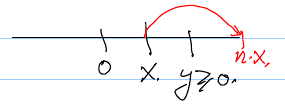
\includegraphics[scale=1]{Illustrations_Analyse/archimedien.png}
\end{wrapfigure}
avec $a,b,c,d > 0$. On choisit $n = (b\cdot c) + 1$\\
$(ad)\cdot n = (ad)\cdot((bc)+1) = (ad)(bc)+(ad)$\\
Donc $n\cdot x = n \frac{a}{b} = n\cdot \frac{ad}{bd} \frac{bc}{bd} = cd = y$

\subsubsection{Démonstration par l'absurde :}
\evid{Proposition} Soit $x \in \Q$, alors $x^2 \neq 2$\\
\evid{Démonstration}(Par l'absurde)\\
Soit $x^2 = 2$, on a $x = \frac{p}{q}, p,q \in \N*, pgcd(p,1) = 1$\\
\begin{align*}
	x^2 = 2 & \Rightarrow \left(\frac{p}{q}\right)^2 = 2\\
			& \Rightarrow  \frac{p^2}{q^2} = 2\\
			& \Rightarrow p^2 = 2q^2\\
			& \Rightarrow (2a)^2 = 2q^2, a \in \N*\mbox{ (p es pair)}\\
			& \Rightarrow 2\cdot 2 \cdot a^2 = 2q^2\\
			& \Rightarrow 2a^2 = q^2\\
			& \Rightarrow 1 = pgdc(p,q)\\
			& \Rightarrow 1 = pgdc(2p,2q) \mbox{ Contradiction !}
\end{align*}
Donc $x^2 \neq 2$ donc l'équation $x^2 = 2$ n'a pas de solution dans $\Q$

\subsection{Les nombres réels $\R$}
\evid{Introduction Axiomatique de $\R$ }\\
On demande de l'ensemble $\R$ la même structure algébrique que pour $\mathbb{Q}$.
\begin{enumerate}
	\item $\R$ est un corps
	\item $\R$ est pourvu d'une relation d'ordre totale,
\end{enumerate}
Puis on demande en plus :
\begin{enumerate}%[resume]
	\item $\R$ a la propriété de la borne inférieure
\end{enumerate}
"Tout sous ensemble non-vide \textit{minoré} de $\R$ admet (dans $\R$) un plus grand \textit{minorant}.\\
\evid{Remarque :} 3 est équivalent à la propriété ``\R a la propriété de la borne supérieure'' ou ``\R a la propriété de la complétude''\\
\evid{Remarque :} \R est \textit{archimédien} (sans démonstration)\\
\evid{Remarque :} L'axiome d'Archimède implique que si $a \in \R$ tel que $0\leq a \leq \frac{1}{n}$ pour tout $n \in \N*$ alors $a = 0$\\
\evid{Remarque :} $\Q \subset \R, \R \setminus \Q :$ les nombres irrationnels.\\

{\setlength{\baselineskip}{3pt}
Existence de $\R^2$\\
\begin{enumerate}
	\item la droite numérique
	\item L'ensemble des nombres à virgule. Attention : $0.999999... \sim 1.000000...$
	\item Des classes d'équivalence des \textit{suites de Cauchy} d'un nombre rationnel
\end{enumerate}}
\begin{boite}
\Definition\\
	Pour avoir la droite numérique achevée, on ajoute deux symboles. $\overline{R} := \R \cup \{-\infty, +\infty \equiv \infty\}$
\end{boite}
\evid{Propriétés}\\
\begin{itemize}
	\item $-\inf < +\infty$
	\item $-\infty < x < \infty  \forall x \in \R$
\end{itemize}
\subsection{Minorants, majorants}
\begin{boite}
	\Definition :\\
	$a\in \R$ est un \textit{minorant} de $\A \cap \R, \A\neq \emptyset$ si $a \leq x \forall x \in \A$
\end{boite}
\begin{boite}
	\Definition :\\
	$a\in \R$ est un \textit{majorant} de $\A \cap \R, \A\neq \emptyset$ si $a \geq x \forall x \in \A$
\end{boite}
\begin{boite}
	\Definition :\\
	$\A \in \R, \A \neq \emptyset$ est \textit{minoré} ou \textit{borné  inférieurement} si $\A$ admet un minorant.
\end{boite}
\begin{boite}
	\Definition :\\
	$\A \in \R, \A \neq \emptyset$ est \textit{majoré} ou \textit{borné  supérieurement} si $\A$ admet un majorant.
\end{boite}
\begin{boite}
	\Definition :\\
	$\A \in \R, \A \neq \emptyset$ est \textit{borné} s'il est majoré ou minoré.
\end{boite}
\begin{boite}
	\Definition :\\
	Un minorant (majorant) $a$ de $\A \subset \R, \A \neq \emptyset$ est appelé \textit{infimum} (\textit{suppremum}) ou \textit{borne inférieur} (\textit{borne supérieur}) si a est le plus grand minorant (plus petit minorant) de $\A$, c'est à dire si tout minorant (majorant) b de $\A$ satisfait la condition $b \leq a$ ($b \geq a$)
\end{boite}
Autrement dit on a :
\begin{enumerate}
	\item $\forall x \in \A$ on a $a := \inf(\A) \leq x$
	\item $\forall \epsilon \in \R, \epsilon > 0$, il existe $x \in \A$ tel que $x \geq a+\epsilon$
\end{enumerate}
\evid{Remarque} $\inf(\A) et \sup(\A)$ existent par définition de \R (axiome 3).
\evid{Remarque} Soit $\A \subset \R, \A \neq \emptyset$, et soit $\mathbf{B} :=\{x\in\R : -x \in \A\}$. Alors $\sup(\A) = -\inf(\A)$\\
\underline{Exemple :}  $\A = \{x \in \R :  1\leq x \leq 2\}$ Alors $\inf(\A) = 1, \sup(\A) = 2$. Voir avec '-\A'
\begin{boite}[0.5]
\Definition (minimum)\\
Si $\inf(\A) \in \A$, alors $\inf(\A) = \min(\A)$
\end{boite}
\begin{boite}[0.55]
\Definition (maximum)\\
Si $\sup(\A) \in \A$, alors $\sup(\A) = \max(\A)$
\end{boite}
\subsubsection{1}
\subsubsection{2}
\subsubsection{Exemples}
\begin{enumerate}
\item $A = \{x \in \R : x < 1\}$. "inf(A) = $-\infty$", sup(A) = 1
\item $A = \{x \in \R : x \leq 1\}$ "inf(A) = $-\infty$, sup(A) = 1 = max(A).
\item $A = \{x \in \R : 0 \leq x, x ^2 < 2\}$, inf(A) = min(A) = 0. sup(A) = $\sqrt{2}$, ou par déf : sup$(A)^2$ = 2.
\end{enumerate}
\underline{Proposition :} a := sup(A) = $\sqrt{2}$ = solution de $x^2 = 2$.\\
$\ulcorner$Soit a = sup(A). On a $1 \in A$ car $1^2 \leq 2$ et donc $a \geq 1$
\begin{enumerate}
\item \underline{supposons que $a^2 < 2$} puisque $\R$ est archimédien. $\exists n \in \N$ tel que $n \cdot (\frac{2-a^2}{2a+1}) > 1 \Leftrightarrow \frac{2a+1}{n} < 2-a^2 < a^2 + 2 - a^2 = 2$\\
\underline{avec de n :} $(a + \frac{1}{n})^2 = a^2 + \frac{2a}{n} + \frac{1}{n^2} \leq a^2 + \frac{2a}{n} + \frac{1}{n}$, et donc $a + \frac{1}{n} \in A$ est en contradiction avec a = sup(A).
\item \underline{supposons que $a^2 > 2$} Puisque $\R$ est archimédien.\\
$\exists n \in \N$ tel que $ n (\frac{a^2 -2}{2a}) > 1 \Leftrightarrow \frac{2a}{n} < a^2 -2 \Leftrightarrow -\frac{2a}{n} > 2-a^2$
\end{enumerate}
\underline{avec ce n :} [trou =3]
1 et 2 impliquent que $a^2 = 2$ car $a^2 \geq 2$ par 1 et $a^2 \leq 2$ ...[trou mika]
\subsubsection{Intervalles (notation}
Soit $a, b \in \R, a \leq b$
\begin{itemize}
\item[Intervalle ouvert] $]a,b[ := \{x \in \R : a < x < b\}$
\item[Intervalle fermé] $[a,b] := \{x \in \R : a \leq x \leq b\}$
\end{itemize}
$]a,a[ = \emptyset$ \\ $]-\infty, \infty[ = \R$ \\ $[-\infty, b] = \{x \in \R : -\infty < x \leq b\}$

\subsubsection{Sous ensembles (générales) de $\R$}
\underline{exemple :} A = [1, 2[ $\cup$ \{3\}
[trou mika]\\
\underline{Définitions :}
\begin{itemize}
\item $E \subset \R$ est ouvert si pour tout $a \in E$ il existe $r > 0$ tel que $]a-r, a+r[ \subset E$.\\
\underline{Exemple :} E = ]0, 1[ est (un ensemble) ouvert. 
\item L'intérieur $\dot{E}$ de E est le plus grand ensemble ouvert contenu dans E. C'est à dire si $A \subset E$,A ouvert, alors $A \subset \dot{E}$
	\item $E \subset \R$ est fermé si $E^c \equiv \R\setminus E$ est ouvert\\
	\underline{exemple :} $E = ]-\infty, 0[ \cup \{1\}\cup [2,\infty[$ est fermé, alors $E^c = ]0, 1[ \cup ]1, 2[$
	\item \underline{L'adhérence $\overline{E}$ de E} est le plus petit sous-ensemble formé de $\R$ qui contient E. C'est à dire si $\R \supset A \supset E$, A fermé, alors $A \supset \overline{E}$. On a $\overline{E} = \R \setminus (\R \setminus E)$ ou encore $\overline{E} = \{a \in \R : \forall r > 0, ]a-r, a+r[ \cap E \neq \emptyset\}$
	\item \underline{le bord $\partial E$ de E} On a $\partial E = \overline{E} \setminus \dot{E}$ ou encore $\partial E = \{a \in \R : \forall r >0, ]a-r, a+r[ \cap E \neq \emptyset$,\\
	$]a-r, a+r[ \cap (\R \setminus E) \}$
	\item $a \in E$ est un point isolé de E s'il existe r > 0 tel que $]a-r,a+r[ \cap E = \{a\}$
	\item \{points limites\} = $\overline{E} \setminus \{$point isolés\}
\end{itemize}

\underline{Remarques :}
\begin{itemize}
\item Soit $E \subset \R$ est borné et fermé, alors inf(E) $\in E$ et sup(E) $\in E$
\item inf et sup d'un ensemble sont uniques
\item $\emptyset, \R$ sont à la fois ouverts et fermés.
\item $E = \dot{E} \Leftrightarrow E$ est ouvert\\
$E = \overline{E} \Leftrightarrow E$ est fermé
\end{itemize}
\subsubsection{Valeur absolue}
\begin{boite}
Définition : pour $x \in \R$ on définit la valeur absolue par $|x| := x \pour x > 0, -x \pour x < 0$
\end{boite}

propriétés :{trou]\\
\underline{inégalité triangulaire :}
$|x+- y| \leq |x| + |y|$\\
$|x+- y| \geq ||x| - |y||$\\
\\
\underline{Identités} (voir les exercices :)\\
$|x + y| + |x-y| = |x| + |y| + ||x| - |y|| = 2max\{|x|, |y|\}$\\
$||x+y|-|x-y|| = |x|+|y|-||x|-|y|| = 2min \{|x|, |y|\}$

\subsection{un truc qu'on verra après}
\subsection{Introduction aux nombres complexes}
\underline{motivation :} Soit $x\in \R$, alors $x^2 + 1 \neq 0$
\subsubsection{Définition du corps des nombres complexes $\mathbb{C}$}
$X = \R \times \R =: \R^2$ donc $(a,b), (c,d) \in X$\\
$\mathbb{C} = \{X, +, \cdot\}$\\
$+ : \mathbb{C} \times \mathbb{C} \longrightarrow \mathbb{C}$\\
$(a,b)(c,d) := (a+c, b+d)$\\
\\
$\cdot  : \mathbb{C} \times \mathbb{C} \longrightarrow \mathbb{C}$\\
$(a,b)(c,d) := (ac-bd, ad+bc)$\\
$\mathbb{C}$ est un corps, appelé le corps ds nombres complexes.
\subsubsection{Représentation cartésienne}
On a $(a,0) + (b,0) = (a+b, o)$\\
on identifie (a,0) $\in \mathbb{C}$ avec a $\in \R$

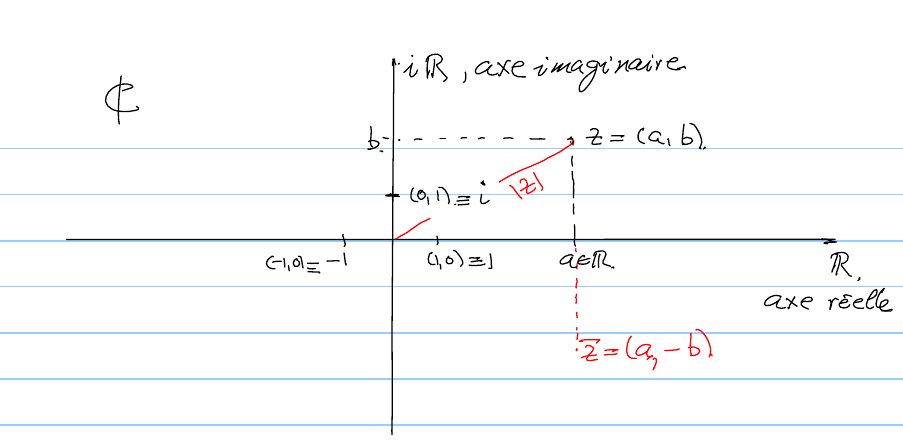
\includegraphics[scale=0.7]{illustrations_Analyse/axes_complexe}
on a $(0,1) [=i] \cdot (0,1) = (0-1, 0+0) = (-1,0) \equiv -1$
\\
\begin{center}
\fbox{\begin{minipage}{0.9\textwidth}
$(0,1) \equiv i$
\end{minipage}}
\end{center}

Donc $i^2 = -1$, ou encore $i^2 + 1 = 0$\\
Pour $z = (a,b) \in \mathbb{C}$\\
$z = (a,0)[\equiv a]\cdot(1,0)[\equiv 1] + (b,0)[\equiv b](0,1)[\equiv i] \equiv a +bi$
\\donc
\begin{center}
\fbox{\begin{minipage}{0.9\textwidth}
$z = a +bi$
\end{minipage}}
\end{center}
C'est la forme ou représentation cartésienne de $z \in \R$
Soit $z_1 = a +bi, z_2 = c+id, a,b,c,d \in \R$\\
En utilisant les règles de calculs "habituelles", plus $i^2 = -1$, on trouve\\
$z_1 + z_2 = (a+ib)+(c+id) = a+c+i(b+d)$\\
$z_1\cdot z_2 = (a+ib) \cdot (c+ib) = (ac-bd)+i(ad+bc)$\\
et on retrouve les opérations + et $\cdot$ de la définition de $\mathbb{C}$
\subsubsection{Définitions}
Soit $z = a+bi \in \mathbb{C}, a,b \in \R$\\
\underline{Complexe conjugué de Z :} $\overline{z} = a-bi \equiv a +i (-b)$
\underline{Propriétés:} \begin{itemize}
\item $\overline{\overline{z}} = z, \forall z \in \mathbb{C}$
\item $\overline{z_1 + z_2} = \overline{z_1} + \overline{z_2}, z_1, z_2 \in \mathbb{C}$
\item $\overline{z_1 \cdot z_2} = \overline{z_1} \cdot \overline{z_2}, z_1, z_2 \in \mathbb{C}$
\end{itemize}
Partie réelle de $z = a+ib$ : $Re(z) \equiv R(z) := a \in \R$\\
Partie imaginaire de $z = a+ ib$ : $Im(z) := b \in \R$\\
\\
\underline{Valeur absolue (ou module) de Z} : $|z| = (z \cdot \overline{z})^{\frac{1}{2}} = \sqrt{z \cdot \overline{z}}$\\
En fait, on a pour $z = ib$\\
$z \cdot \overline{z}= (a+ib)(a-ib) = a^2 - b^2 \geq 0$\\
\\
\begin{center}
\fbox{\begin{minipage}{0.3\textwidth}
\underline{Remarque :} \\
$Re(z) = \frac{z \cdot \overline{z}}{2} \in \R$\\
$Im(z) = \frac{z \cdot \overline{z}}{2i} \in \R$
\end{minipage}}
\end{center}
\subsubsection{Élément inverse pour la multiplication}
Soit $z \in \mathbb{C}, z \neq 0$, On cherche $z \in \mathbb{C}$ tel que $z \cdot \overline{z} = 1 \in \R \subset \mathbb{C}$\\
\\
On a $z_1 = \frac{1}{|z|^2}\overline{z}$\\
En effet $z \cdot z_1 = z \cdot \frac{1}{|z|^2}\overline{z} = \frac{1}{|z|^2} \overline{z}\cdot z$ or $\overline{z} \cdot z = |z|^2$ par définition, alors = 1\\
\\
\underline{Notation pour l'inverse} $\frac{1}{z}$ ou $z^{-1}$\\
\underline{Remarque :} "$\frac{1}{z} = \frac{1}{z} \cdot \frac{\overline{z}}{\overline{z}} = \frac{1}{z \cdot \overline{z}}\overline{z} = \frac{1}{|z|^2} \cdot \overline{z}$"\\
\\
\underline{explicitement, pour z = ib}
[trou cours]...$=\frac{ac+bd}{c^2+d^2} + i\cdot\frac{bc-ad}{c^2+d^2}$
\subsubsection{Formules d'Euler et de Moïvre}
Soit $\varphi \in \R$. 
\begin{boite}[0.65]
On pose $e^{i\varphi} = \cos(\varphi) + i \sin(\varphi)$ Formule d'Euler
\end{boite}
avec les règles de calcul habituelles pour la fonction exponentielle :\\
\\
\underline{pour $z_1, z_2 \in \mathbb{C}$} : $e^{z_1} \cdot e^{z_2} = e^{z_1+z_2}$\\
$(e^z)^n = e^{nz}$ pour $n \in \N*$\\
ainsi que $\overline{e^z} = e^{\overline{z}}$\\
\\
avec $z = a +ib$, $e^z = e^{a+ib} = e^i + e^{ib}$\\
$e^a \in \R$ (exponentielle réelle)\\
$e^{ib} = \cos(b) + i\sin(b)$\\
$Re(e^{a+ib}) = e^a\cos(b ), Im(e^{a+ib}) = e^a\sin(b)$\\
On a aussi (Euler et règles pour Re, Im)\\
$\cos(\varphi) = Re(e^{i\varphi} = [trou cours]$\\
\underline{Formule de Moïvre :}
Pour $n \in \N*, \varphi \in \R$, on a\\
$\cos(n\varphi) + i\sin(n\varphi) = e^{i n \varphi} = (e^{i\varphi})^n = (\cos(\varphi) + i\sin(\varphi))^n$
[trou cours]
$n = 3$ : $\sin(3\varphi) = Im(\cos(\varphi) + i(\sin(\varphi))^3 = \cos(\varphi)^2\cdot \sin(\varphi) - \sin(\varphi)^3$
\subsubsection{Forme polaire d'un nombre complexe}
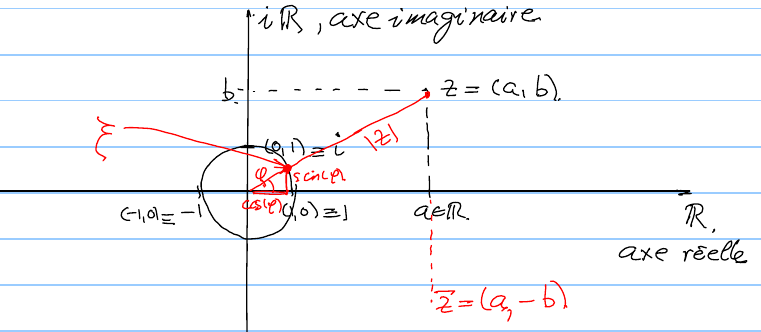
\includegraphics[scale=0.5]{illustrations_Analyse/cercle_polaire}

$z \neq 0$, $z = |z|\cdot\zeta$ où $\zeta = \frac{1}{|z|}z$, $|\zeta| = \frac{1}{|z|}|z| = 1$.

$\zeta = \cos(\varphi) + i\sin(\varphi) = e^{1\varphi}$\\
Donc tout $z \neq 0$ est de la forme 

\textcolor{red}{\begin{equation}
a+ib = z = |z| \cdot e^{i\varphi}
\end{equation}}

où $\varphi =2 \arctan(\frac{b}{1+\sqrt{a^2 + b^2}})$si $z \in \mathbb{C}\setminus ]-\infty, 0]$ (ou $\pi$ sinon)\\
la forme ou la représentation polaire de z.
\begin{boite}
\underline{Définition :} Le nombre $\varphi \in ]-\pi, \pi]$ est appelé l'argument de $z \in \mathbb{C}, \varphi = \arg(z)$\\
$arg(z)= \varphi= \left\{
    \begin{array}{lr}
        2\cdot \arctan\frac{y}{y+\sqrt{y^2+x^2}} & \mbox{si } y \neq 0 \mbox{ et si } x>0, y>0\\
        \pi & \mbox{si } x<0, y = 0
    \end{array}
\right.
$
\end{boite}

la forme polaire est mieux adaptée à la multiplication des nombres complexes. Soit $z_1, z_2 \in \mathbb{C*} \equiv \mathbb{C} \setminus \{0\}$, alors\\
$z_1 = |z_1|\cdot e^{e\varphi_1}, z_2 = |z_2|\cdot e^{i\varphi_2}$
et 
\textcolor{red}{\begin{equation}
z_1\cdot z_2 = |z_1|\cdot|z_2| e^{i(\varphi_1 + \varphi_2)}
\end{equation}}

Soit $r > 0, \varphi \in \R$. L'inverse :\\
$z = r\cdot e^{i\varphi}$\\
$= r (\cos(\varphi) + i\sin(\varphi))$\\
$= r\cos(\varphi) + i\cdot r \cdot \sin(\varphi)$\\

$\frac{1}{z} = \frac{1}{r e^{i\varphi}} = \frac{1}{r} e^{-i\varphi} = \frac{1}{e^{i\varphi}}$
\subsubsection{Exemples}
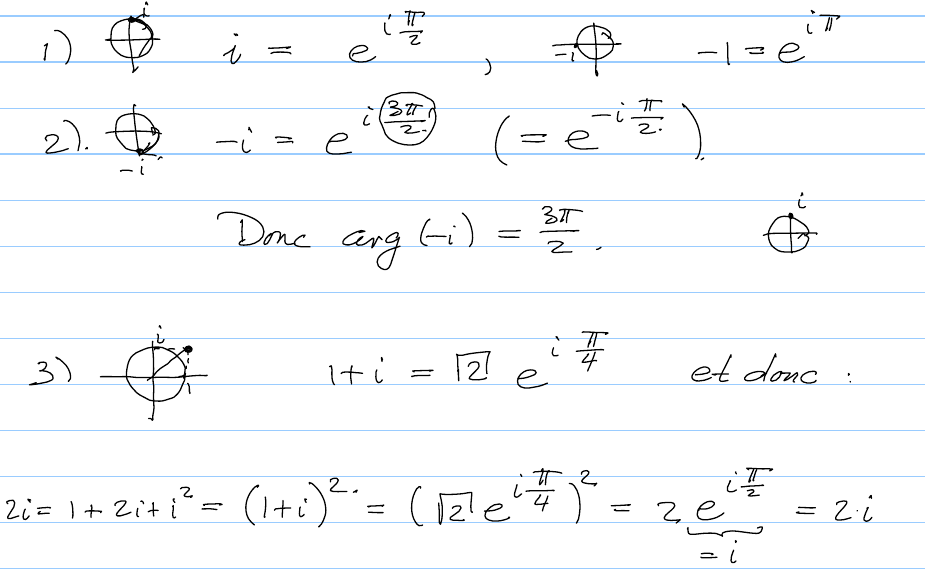
\includegraphics[scale=0.5]{illustrations_Analyse/exemples_1_3}\\
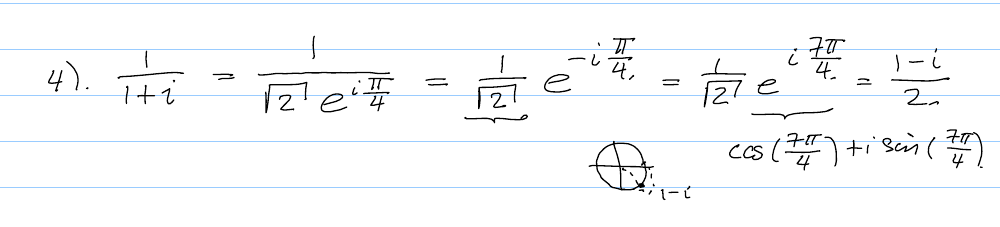
\includegraphics[scale=0.60]{illustrations_Analyse/exemple_4}\\
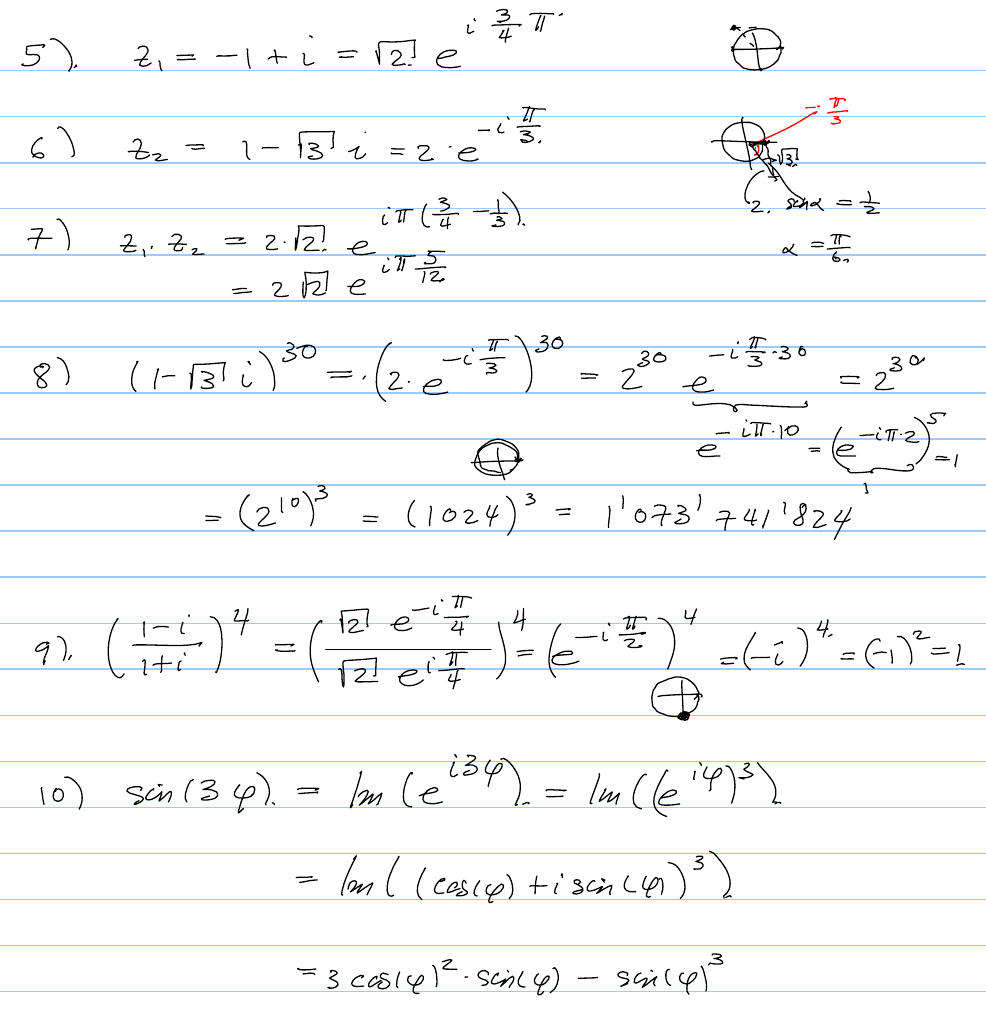
\includegraphics[scale=0.60]{illustrations_Analyse/exemples_5_10}

\subsubsection{La fonction et sa réciproque }
Soit $z = r\cdot e^{i\varphi}, r > 0, \varphi \in ]-\frac{\pi}{2}, \frac{\pi}{2}[$\\
$z^2 = r^2 \cdot e^{12\varphi}, 2\varphi  \in ]-\pi, \pi[$
%[trou dessin]

\[
z = \sqrt{\omega} =
\left\{
\begin{array}{l c l r}
\sqrt{\omega} = \sqrt{x}  & $pour$ & y = 0, x > 0 & $cas 1$\\
\frac{1}{\sqrt{2}}(\sqrt{|\omega| + x} + i \sqrt{|\omega| -x}) & $pour$ & y > 0 & $cas 2$\\
\frac{1}{\sqrt{2}}(\sqrt{|\omega| + x} - i\sqrt{|\omega| - x}) & $pour$ & y < 0 & $cas 3$
\end{array}
\right.
\]
Cas 2 $(\frac{1}{\sqrt{2}}(\sqrt{|\omega| + x} + i\sqrt{|\omega| - x}))^2 = \frac{1}{2} (|\omega| + x - |\omega| + x + 2i \sqrt{\omega^2 - x^2}) = x + iy$

\subsection{Résolution des équations}
\subsubsection{"Racines" n-ièmes}
Dans $\mathbb{C}$, l'équation 
\begin{equation}
z^n = \omega \in \mathbb{C}, n \in \mathbb{N*}
\end{equation}
a toujours n solutions si $\omega \neq 0$. $z = \omega$ est la seule solution pour $\omega = 0$\\
\\
\underline{Méthode "polaire"}

\begin{itemize}
\item $\omega = |\omega|\cdot e^{i(\varphi + k2\pi)}$, avec $k = 0,...,n-1$
\item $z_k = |\omega|^{\frac{1}{n}} \cdot e^{i(\frac{\varphi}{n} + \frac{k}{n}\cdot 2\pi)}$ avec $k = 0,...,-n1$
\end{itemize}
\underline{Exemples}
\begin{itemize}
\item $z^2 = 1 = e^{i(0+k2\pi)}$ avec $ k = 0,1$\\
$z_k = e^{1\frac{k}{2}2\pi}$ avec $k = 0,1$\\
$z_0 = e^0 = 1, z_1 = e^{i\pi} = -1$
\item $z^3 = 1 = e^{i(0 + k2\pi)}$ avec $k = 0,1,2$\\
$z_k = e^{1\frac{k}{3}2\pi}$ avec $k = 0,1,2$\\\\
$z_0 = e^0 = 1, z_1 = e^{\frac{2\pi}{3}}, z_2 = e^{i\frac{4\pi}{3}} = e^{-i\frac{2\pi}{3}}$
\item %[trou c
$z^3 = i = e^{i(\frac{\pi}{2} + 2\pi k}$, k = 0,1,2\\
$z_0 e^{i\frac{\pi}{6}} = \frac{\sqrt{3}}{2} + i\frac{1}{2} $\\
$z_1 = e^{i(\frac{\pi}{6} + \frac{2\pi}{3})} = e^{i\frac{5\pi}{6}} = -\frac{\sqrt{3}}{2} + i \frac{1}{2}$\\
$z_2 = e^{i(\frac{\pi}{6} + \frac{4\pi}{3})} = e^{i\frac{3\pi}{2}} = -i$
\item $z^6 = 1+i = \sqrt{2}\cdot e^{i(\frac{\pi}{2} + k2\pi}$, k = 0-5\\
$z_k = 2^\frac{1}{12}e^{i(\frac{\pi}{24} + \frac{k}{6}\pi}$
\end{itemize}

\subsubsection{Le cas n = 2 (méthode cartésienne)}
Le cas $z^2 = \omega = x + iy$.\\
$y = 0, x \geq 0 \to z_0 = \sqrt{x}$ et $ z_1 = -\sqrt{x}$\\
$y = 0, x < 0 \to z_0 = i\sqrt{|x|}$ et $ z_1 = -i\sqrt{|x|}$\\
$y \neq 0 \to z_0 = \sqrt{\omega}, z_1 = -\sqrt{\omega}$\\
\\
avec $\sqrt{.}$ la fonction réelle (y = 0) ou complexe ($y \neq 0$)\\
\\
Puisque $z^2 + pz + q = (z + \frac{p}{2})^2 - (\frac{p}{2})^2 + q$ l'équation $z^2 + pz + q = 0$ peut 
[trou mika]
\subsubsection{Théorème fondamental de l'algèbre}
Tout polyne p(z) = $a_nz^n+...+a_iz^i + a_0, n\in \mathbb{N*} a_0,...a_n \in \mathbb{C}, a_n \neq 0$ admet dans $\mathbb{C}$ n "racines" c'est à dire il existent $z_0,...z_n \in \mathbb{C}$ tels que $p(z_k) = 0, k = 0,...n-1$ et on a la représentation 
$p(z) = a_n (n_n-z_0)...(z-z_n-1)$\\
\\
\underline{Exemples :}
\\
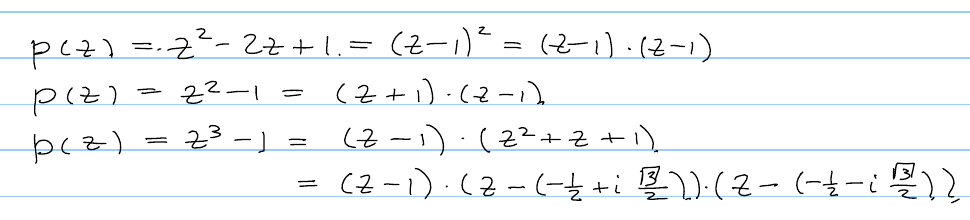
\includegraphics[scale=0.5]{illustrations_Analyse/exemples_z}

\subsubsection{Quelques résultats généraux}
Si les $a_k$ sont réels (polynôme réel), alors $\overline{p(z)} = p(\overline{z})$ (vérifier. Dans ce cas, $p(\overline{z_k} = 0$  si $p(z_k) = 0, car \overline{0} = 0$.

Explication : ou bien $z_k \in \R$ et on a un facteur réel, ou $z_k \not \in \R$ ce qui donne des facteurs complexes conjugués $(z-z_k)(z-\overline{z_k})$

Théorème : Tout polynôme à coefficients réels peut être factorisé dans $\R$ en facteurs linéaires ou quadratiques

Explication : $(z-z_k)(z-\overline{z_k}) = (z^2 - (z + \overline{z_k})-z + z_k \overline{z_k}$

\section{Suite de nombres réels}
\setcounter{equation}{0}
\begin{boite}
\underline{Définition :} On appelle suite de nombres réels toute application $f:\N \to \R$
\end{boite}
\underline{Notation :} On pose $a_n = f(n)$ et on écrit $(a_n)$ ou $(a_n)_{n \geq 0}$ ou $a_0, a_1,...$ pour la suite \\
\underline{Remarque :} On écrira $(a_n)_{n \geq n_0}$ pour une suite numérotée par $n_0,n_{0+1},...$\\

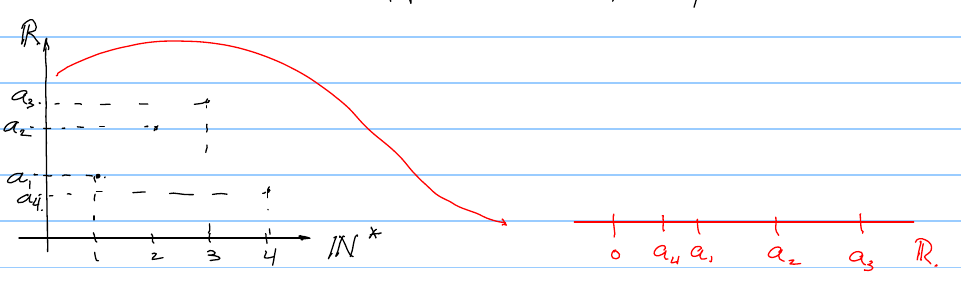
\includegraphics[scale=0.65]{illustrations_Analyse/graphe_suite}

\underline{On s'intéresse à l'image de f :} $Im(f) = \{x \in \R : x = a_n$ pour un $n \in \N$\} = $\{a_0,a_1,a_2,...\}$
\subsection{Exemples :}
\subsubsection{Suite harmonique}
$a_n = \frac{1}{n}, n \in  \mathbb{N*}$\\
$a_1 = 1, a_2 = \frac{1}{2}, a_3 = \frac{1}{3},...$\\
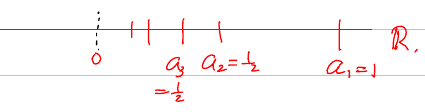
\includegraphics[scale=1]{illustrations_Analyse/suite_harmonique}
\subsubsection{Suite harmonique alternée}
$a_n = (-1)^{n-1}\cdot\frac{1}{n}, n \in \mathbb{N*}$\\
$a_1 = 1, a_2 = -\frac{1}{2}, a_3 = \frac{1}{3}, a_4 = -\frac{1}{4},...$\\
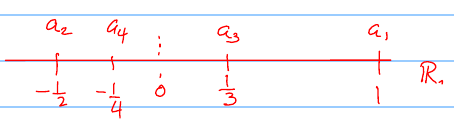
\includegraphics[scale=1]{illustrations_Analyse/suite_harmonique_alternee}
\subsubsection{Suite arithmétique}
$a_n  =a_1 + (n-1)\cdot d, a,d \in\R, n \in \N$\\
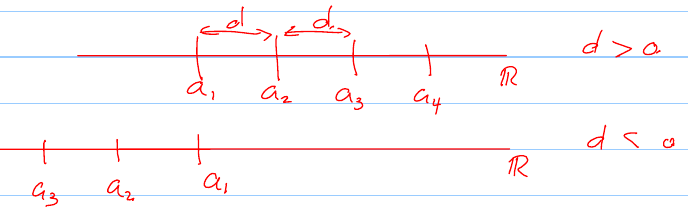
\includegraphics[scale=1]{illustrations_Analyse/suite_arithmetique}
\subsubsection{Suite géométrique}
$a_n = a_1 \cdot q^{n-1}, a,q\in \R, q \neq 0, n\in \mathbb{N*}$
\begin{itemize}
\item Si q = 1 : $a_n = a1$ pour tout $n \in \N$
\item si q = -1 : 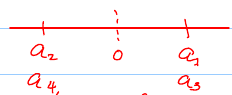
\includegraphics[scale=0.5]{illustrations_Analyse/suite_geometrique}
\item si $q > 1 $ 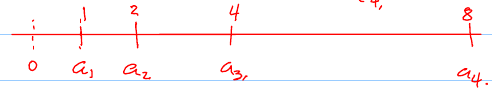
\includegraphics[scale=0.5]{illustrations_Analyse/suite_geometrique_geq_1} pour a=1, q=2
\item si $q < 1$ : 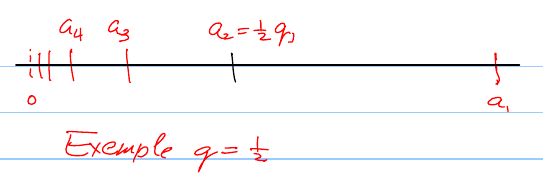
\includegraphics[scale=0.5]{illustrations_Analyse/suite_geometrique_leq_1}
\end{itemize}
\subsection{Suites définies par récurrence}
Soit $a_1 \in \R$ et soit $g : \R \to \R, \mathbf{D}(g) = \R$\\
$a_n = g(a_{n-1}), n = 2,3,4,...$\\
\\
\underline{Exemples :}

\begin{itemize}
\item $g(x) = x+d \Rightarrow a_{n+1} = a_n + d$ Suite arithmétique (démonstration par récurrence)
\item $g(x) = x \cdot q \Rightarrow a_{n+1} = a_n \cdot q$ suite géométrique (démonstration par récurrence également)\\
	\begin{flushleft}
		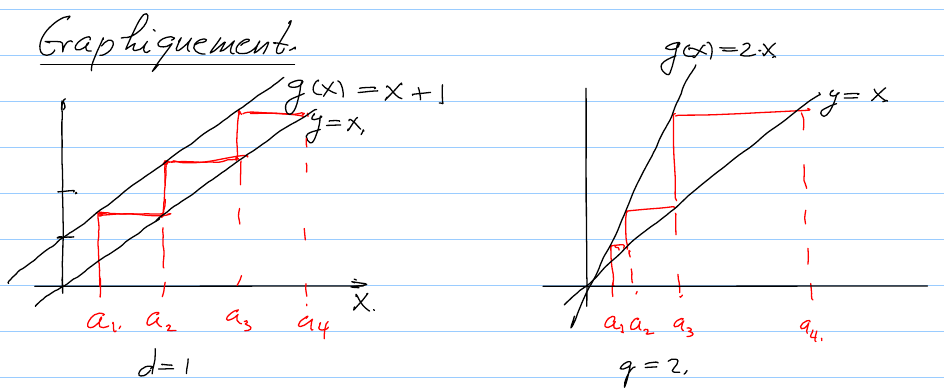
\includegraphics[scale=0.7]{illustrations_Analyse/graph_suite_geom}
	\end{flushleft}	
\item $g(x) = \frac{x}{x+1}$ pour $a_1 = 1$ on obtient la suite harmonique.\\
démonstration par récurrence :\\
\begin{itemize}
	\item $a_1 = 1, a_2 = \frac{1}{1+1} = \frac{1}{2}$
	\item $g(a_{n-1}  P(n-1). g(\frac{1}{n-1}) = \frac{\frac{1}{n-1}}{1+\frac{1}{n-1}} = \frac{1}{n} = a_n$
\end{itemize}
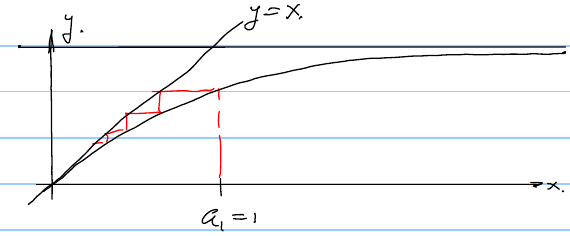
\includegraphics[scale=0.5]{illustrations_Analyse/graph_suite_harmo}
\item $a_1 = \sqrt{2}, g(x) = (\sqrt{2})^x = (1.414...)^x$\\
$a_n = (\sqrt{2})^{a_{n-1}}$\\
$a_1 = \sqrt{2}= 1.414..., a_2 = \sqrt{2}^{\sqrt{2}} = 1.63..., a_3 = \sqrt{2}^{(\sqrt{2}^{\sqrt{2}})},...a_{10} = 1.983..., a_{1000} = 1.999...$\\
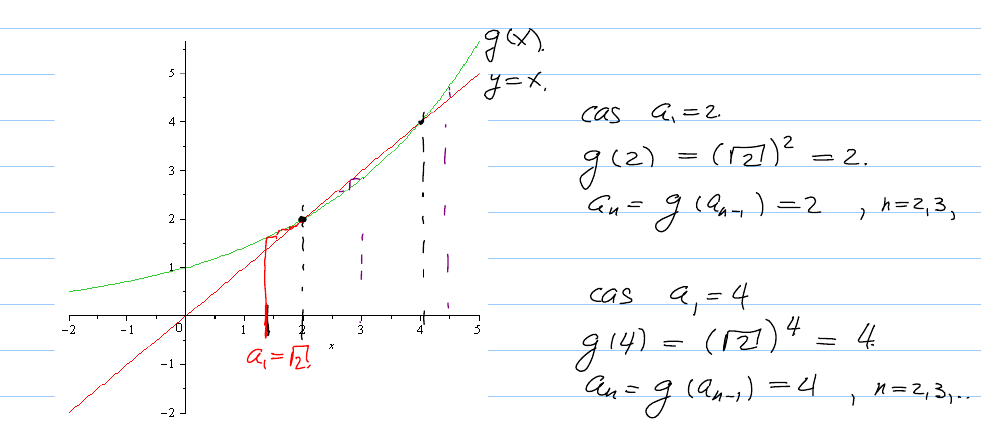
\includegraphics[scale=0.5]{illustrations_Analyse/sqrt2}
\end{itemize}
\subsection{Définitions}
\underline{Suite croissante} une suite ($a_n$) est croissante si $a_{n+1} \geq a_n, \forall n \in \N$\\
\\
\underline{Suite décroissante} une suite ($a_n$) est décroissante si $a_{n+1} \leq a_n, \forall n \in \N$\\
\\
\underline{Suite monotone} Une suite ($a_n$) est monotone si elle est soit croissante, soit décroissante.\\
\\
\underline{Suite majorée} Une suite ($a_n$) est majorée si $E = \{a_0,a_1.---\} \subset \R$ est majoré\\
\\
\underline{Suite minorée} Une suite ($a_n$) est minorée si $E = \{a_0,a_1.---\} \subset \R$ est minoré\\
\\
\underline{Suite bornée} Une suite ($a_n$) est bornée si elle est minorée \underline{\underline{et}} majorée\\
\\
\underline{Plus petit majorant d'une suite} sup($a_n$) := sup$\{a_0,a_1,a_2,...\}$\\
\\
\underline{Plut grand minorant d'une suite} inf($a_n$) := inf$\{a_0,a_1,a_2,...\}$\\
\\
\underline{Minimum et maximum d'une suite}\\
max($a_n$) := max$\{a_0,a_1,a_2,...\}$ s'il existe\\
min($a_n$) := min$\{a_0,a_1,a_2,...\}$ s'il existe\\
\\
\\
\underline{Exemple 2.3}\\
$a_n = 1+ \frac{1}{n}, n \in \N
, a_1 = 2, a;2 = \frac{3}{2}$\\
$1\leq a_n \leq 2$ La suite est bornée\\
sup($a_n$) = max ($a_n$) = 2\\
inf($a_n$) = 1, pas de minimum.

\subsection{Limite d'une suite}
\begin{center}
\fbox{\begin{minipage}{0.9\textwidth}
\underline{Définition :} une suite ($a_n$ est convergente et admet pour limite (ou converge vers) $a \in \R$ et l'on écrit
\begin{equation}
\lim\limits_{n \to \infty}a_n = a
\end{equation}
si pour tout $\epsilon > 0$ il existe $n_0$ tel que $|a_n-a| < \epsilon, \forall n \geq n_0$
\end{minipage}}
\end{center}
\underline{remarque :} $\Rightarrow a$ est un point adhérent à $\{a_0,a_1,...\}$\\
\underline{remarque :} $|a_n-a| < \epsilon \Leftrightarrow a-\epsilon < a_n < a+\epsilon$\\
\underline{remarque :} La démonstration dans l'exemple 2.3 montre que la suite $a_n = 1 + \frac{1}{n}$ converge vers a = 1, car $\forall \epsilon > 0$ on a  $1 \leq a_n \leq 1 + \epsilon, \forall n \geq n_0 > \frac{1}{\epsilon}$

\underline{Notations équivalentes}\\
$\limite{n \to \infty} a_n = a\in \R \Leftrightarrow a_n \to a \Leftrightarrow a:n \to a$ lorsque $n \to \infty$\\
\\
\underline{exemples :}\\
\begin{enumerate}
\item $\limite{n \to \infty} (1+\frac{1}{n} = 1$
\item $\limite{n \to \infty} \frac{1}{n} = 0$ même demonstration que dans l'exemple 2.3
\item $\limite{n \to \infty} \underbrace{(-1)^n}_{a_n}$ pas de limite
\end{enumerate}

\underline{Proposution :} Si une suite converge, sa limite est unique.\\
\\
\underline{Démontration par l'absurde}\\
oit $\limite{\ninf} = a \text{ et } \limite{\ninf} a_n = b \text{ avec } b \neq a$
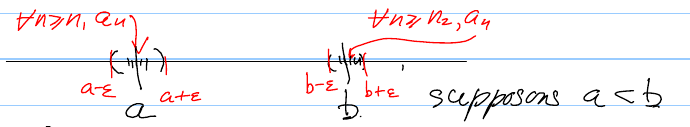
\includegraphics[scale=0.5]{illustrations_Analyse/suite_converge}\\
Soit $\epsilon \leq \frac{1}{3} (b-a)$\\
$\limite{\ninf} a_n = a \Leftrightarrow \exists n_1 t.q. \forall n \geq n_1 |a-a_n| < \epsilon$\\
$\limite{\ninf} a_n = b \Leftrightarrow \exists n_2 t.q. \forall n \geq n_2 |b-a_n| < \epsilon$\\
Soit $n_0 = \max\{n_1, n_2\}$, alors pour $n \geq n_0$ on a \\
$|a-a_n| < \epsilon \text{ \underline{ET} } |b-a_n| < \epsilon$\\
Donc $|b-a| = |(b-a_n) - (a-a_n)| \leq |b-a_n| + a-a_n| \leq \epsilon + \epsilon \leq \frac{2}{3}|b-a|$\\
Donc $0\leq \frac{1}{3}|b-a| \leq 0$\\
Donc $b-a = 0 \to b = a$

\subsection{Suite divergentes et fortement divergentes}
\begin{center}
\fbox{\begin{minipage}{0.9\textwidth}
\underline{Définition :} Une suite ($a_n$) qui n'est pas convergente est appelée divergente.
\end{minipage} }
\end{center}
\underline{Exemple :} $a_n = (-1)^n, n \in \N$ est une suite divergente.
\underline{Suites "fortement divergentes"}
\begin{center}
\fbox{\begin{minipage}{0.9\textwidth}
\underline{Définition :} Soit $(a_n)$ une suite telle que pour tout $r \geq 0$ il existe $n_0$ tel que $\forall n \geq n_0, a_n \geq r$ alors on écrit $\limite{\ninf} a_n = \infty$
\end{minipage} }
\end{center}
\underline{Exemple :} $\limite{\ninf} n = \infty$
\begin{center}
\fbox{\begin{minipage}{0.9\textwidth}
\underline{Définition :} Soit $(a_n)$ une suite telle que pour tout $r > 0$ il existe $n_0$ tel que $\forall n \geq n_0, a_n \leq r$, alors on écrit $\limite{\ninf} a_n = -\infty$
\end{minipage} }
\end{center}

\underline{Exemple :} $\limite{\ninf} -n = -\infty$

\begin{center}
\fbox{\begin{minipage}{0.9\textwidth}
\underline{Attention :}Par abus de langage, on dit souvent que la suite $(a_n)$ "converge" vers $\infty$ ou $-\infty$ si $\limite{\ninf} a_n = \infty$ ou $\limite{\ninf} a_n = -\infty$
\end{minipage} }
\end{center}

\underline{Remarque :} La suite $a_n = (-1)^n \cdot n$ diverge, et elle ne "converge" pas non plus vers $\infty \text{ ou }-\infty$

\subsection{Opérations algébriques sur les limites}
Si ! $\limite{\ninf} a_n = a\in \R, \limite{\ninf} b_n = b \in \R, \text{ et } \alpha, \beta \in \R$\\
alors (à vérifier en utilisant les définitions !)\\

\begin{itemize}
\item $\limite{\ninf} (\alpha a_n + \beta b_n) = \alpha \limite{\ninf} a_n + \beta \limite{\ninf} b_n = \alpha a + \beta b$
\item $\limite{\ninf} (a_n \cdot b_n) = (\limite{\ninf} a_n) \cdot (\limite{\ninf}b_n) = a\cdot b$
\item $\limite{\ninf}(\frac{a_n}{b_n}) = ... = \frac{a}{b} \text{ si } b_n \neq 0, b \neq 0$
\end{itemize}

\underline{Conséquences :} $\limite{\ninf} a_n = a \Leftrightarrow \limite{\ninf}(a_n \underbrace{-a}_{a_n}) = 0$\\
\underline{Exemples :} 
$\limite{\ninf}\frac{2n+3}{3n-5} = 
\limite{\ninf}\frac{2n\cdot (1+ \frac{3}{2n})}{3n(1-\frac{5}{3n})} = 
\limite{\ninf}(\frac{2}{3} \frac{1+\frac{3}{2n}}{1-\frac{5}{3n}}) = 
\frac{2}{3} \limite{\ninf} \frac{1+ \frac{3}{2n}}{1- \frac{5}{3}} = 
\frac{2}{3} \frac{\limite{\ninf}(1+ \frac{3}{2n})}{\limite{\ninf} (1-\frac{5}{3n})} =
\frac{2}{3} \frac{\limite{\ninf} 1 + \frac{3}{2}(\limite{\ninf}\frac{1}{n})}{(\limite{\ninf}1) - \frac{5}{3} (\limite{\ninf}\frac{1}{n})} 
= \frac{2}{3} \frac{1+\frac{3}{2}0}{1-\frac{5}{3}0} = \frac{2}{3}$\\
\\
\underline{Attention aux hypothèses:}\\
$1 = \limite{\ninf} 1 = \limite{\ninf} \frac{n}{n} = \frac{\limite{\ninf} n}{\limite{\ninf} n} = \frac{\infty}{\infty}$\\
\\
\underline{Manipulation de $\infty$ et 0 :}\\
\begin{itemize}
\item$\infty + \infty = \infty$
\item$\infty\cdot\infty = \infty$
\item$\frac{0}{\infty} = 0$
\item$c + \infty = \infty$
\item$\frac{c}{\infty} = 0 \forall c \in \R$
\item$c \cdot\infty = \infty, c > 0$
\end{itemize}

\subsection{Théorème des deux gendarmes}
\begin{center}
\fbox{\begin{minipage}{0.9\textwidth}
\underline{Théorème :} Soit $(a_n), (b_n), (c_n)$, trois suites telles que $a_n \leq c_n \leq b_n, \forall b \geq n_o \in \N, \limite{\ninf} a_n = a, \limite{\ninf} b_n = a$, alors $\limite{\ninf}c_n = a$
\end{minipage} }
\end{center}
\underline{Démonstration : }\\
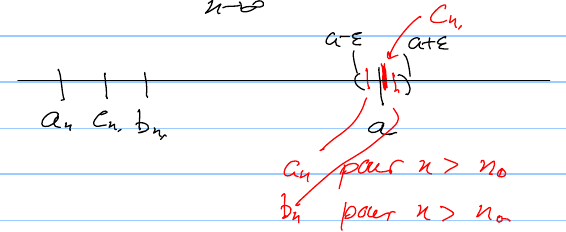
\includegraphics[scale=0.5]{illustrations_Analyse/gendarmes}\\
$\forall \epsilon > 0, \exists n_o$ tel que $|a_n-a| \leq \epsilon \text{ et } |b_n -a| \leq \epsilon$\\
Donc 
\begin{equation}
\underbracket{-\epsilon} \leq a_n -a \leq \underbracket{c_n -a} \leq b_n -a \leq \underbracket{\epsilon}
\end{equation}
$\Rightarrow |c_n -a| \leq \epsilon$\\
\\
\underline{Exemples :}\\
\begin{itemize}
\item $a_n := \underbrace{\underbrace{\frac{-1}{n^2 + 1}}_{n \to \infty, \text{ donc } 0} \leq c_n = \frac{\cos(7n^2+3)}{n^2 + 1}  \leq \underbrace{\frac{1}{n^2 + 1}}_{n \to \infty, \text{ donc } 0}}_{\text{donc } c_n = 0}$
\item $a_n := \underbrace{\underbrace{1}_{\mathclap{n \to \infty, \text{ donc } 1}} \leq c_n = \sqrt{1+\frac{1}{n}} \leq \sqrt{1+\frac{2}{n} + \frac{1}{n^2}} = \underbrace{1 + \frac{1}{n}}_{\mathclap{n \to \infty, \text{ donc } 1}}}_{1}$
\item %[TROU COURS]
\end{itemize}

\subsection{Critères de convergence}
\begin{center}
\fbox{\begin{minipage}{0.9\textwidth}
\underline{Théorème :} Toute suite \underline{croissante et majorée (décroissante et minorée)} est convergente et $\limite{\ninf} a_n = \sup(a_n)$ (et $\limite{\ninf}a_n = \inf(a_n))$
\end{minipage} }
\end{center}
\begin{center}
\fbox{\begin{minipage}{0.9\textwidth}
\underline{Corollaire :} Toute suite monotone et bornée est convergente
\end{minipage} }
\end{center}
\underline{Démonstration }(pour le sup, pur l'inf voir l'Exemple 2.3\\
%[dessin]
\begin{itemize}
\item $\forall \epsilon > 0, \exists n_0$ tel que $a_{n_0} > a-\epsilon$ par définition du sup.
\item $\forall n a_n \leq a$ Par définition du sup
\item$a_n \geq a_{n_o}, \forall n \geq n_0$ car la suite est croissante
\end{itemize}
Donc : $ \forall \epsilon > 0, \exists n_0$ tel que $\forall n \geq n_0, a-\epsilon \leq a_{n_0} \leq a_n \leq a \leq a + \epsilon$\\
C'est à dire $|a_n-a| < \epsilon$ et donc $\limite{\ninf} a_n =a$ par définition de la suite.

\begin{boite}
\underline{Rappels :}\\
$\begin{pmatrix}
n \\ 
k
\end{pmatrix}
= \frac{n!}{k!(n-k)!} = \frac{n(n-1)...(n-k+1)}{k!}, 0! = 1$\\
$(A+B)^n = \sum^{n}_{k=0} \begin{pmatrix}
n \\ 
k
\end{pmatrix}
A^{n-k}B^k = A^n + nA^{n-1}B+...$\\
$\sum^{n-1}_{k=0}a^k = \frac{1-a^n}{1-a}$
\end{boite}
\underline{Exemple :} (majoré + croissant $\Rightarrow$ converge)\\
$a^n = (1 + \frac{1}{n})^n, n \in \mathbb{N*}$ (série 6, exo 6)\\
\begin{enumerate}
\item[La suite est majorée] $a_n = 1 + \sum_{k=1}^{n} \begin{pmatrix}
n\\
k
\end{pmatrix}
=(\frac{1}{n})^k = 1 + \sum_{k=1}^n \frac{n(n-1)...(n-k+1)}{k!}(\frac{1}{n}^k$\\
$=1 + \sum_{k=1}^n\frac{1}{k!} 1(1-\frac{1}{n})...(1- \frac{k-1}{n}$\\
$\leq 1 + \sum_{k=1}^n \frac{1}{k!} \leq 1 + \sum_{k=1}^n \frac{1}{2^{ k-1}} = 1 + \sum_{k=1}^n (\frac{1}{2})^k$\\
$k! = 1\cdot 2...\cdot k \geq 2^k-1$\\
$=1 +  \frac{1-(\frac{1}{2})^n}{1 - \frac{1}{2}} \leq 1 + \frac{1}{1- \frac{1}{2}} = 3$
\item[La suite est croissante] $a_n = 1 + \sum_{k=1}^n \frac{1}{k!} 1 (1-\frac{1}{n})...(1-\frac{k-1}{n}$\\
$\leq 1 + \sum_{k=1}^n \frac{1}{k!} 1(1-\frac{1}{n+1})...(1-\frac{k-1}{n+1}) + \frac{1}{(n+1)!}1(1-\frac{1}{n+1})...(1-\frac{n}{n+1}) = a_{n+1}$
\end{enumerate}
1+2  implique que $\limite{\ninf} (1+\frac{1}{n})^n := e = 2.718..$ (nombre d'Euler)
\subsection{Convergence d'une suite définie par récurrence (un exemple)}
$a_1 = 3, a_n = g(a_{n-1}), n = 2,3, g(x) = \frac{1}{2}x + \frac{5}{2}\frac{1}{x}$\\
c'est à dire : $a_n = \frac{1}{2} a_{n-1} + \frac{5}{2}\frac{1}{a_{n-1}}$\\
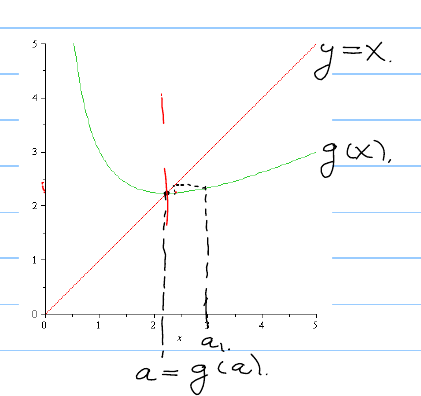
\includegraphics[scale=0.5]{illustrations_Analyse/suite_recurrence}\\
\underline{Montrons que l asuite est minorée et décroissante (converge)}
\begin{enumerate}
\item $a_n > 0, \forall n \in \mathbb{N*}$ (éa suite est bien définie)\\
par récurrence : $a_1 = 3  > 0 \to a_n > 0$ si $a_{n-1} > 0, n=2...$
\item On calcule la limite sous l'hypothèse qu'elle existe\\
$a = \limite{\ninf} a_n = \frac{1}{2} \limite{\ninf} a_{n-1} + \frac{5}{2} \frac{1}{\limite{\ninf} a_{n-1}} = \frac{1}{2} a  + \frac{5}{2}\frac{1}{a}$\\
$\Rightarrow \frac{1}{2}a^2 - \frac{5}{2} = 0 \Rightarrow a = \sqrt{5}$ ($-\sqrt{5}$ n'est pas posible)
\item La suite est minorée par $\sqrt{5} (\sqrt{5} = \inf(a_n)$\\
Démonstration par récurrence ($P_n : a_n \geq \sqrt{5}$)
\begin{itemize}
\item $a_1 = 3 \geq \sqrt{5}$
\item $a_n = \frac{1}{2}(a_{n-1} + \frac{5}{<_{n-1}} = \frac{1}{2a_{n_1}}(a_{n-1}^2 + 5) = \frac{1}{2a_{n-1}}(a_{n-1} - \sqrt{5})^2 + \sqrt{5} \geq \sqrt{5} (P_n)$
\end{itemize}
\item La suite est décroissante (car $a_n \geq \sqrt{5}$ ou par récurrence)\\
$a_n - a_{n-1} = \frac{1}{2}a_{n-1} + \frac{5}{2} \frac{1}{a_{n-1}} = \frac{-a_{n-1}^2 + 5}{2\cdot a_{n-1}} \leq 0$\\
\end{enumerate}
$2+\underbrace{3+4}_{\mathclap{\text{série convgergente}}}$ : $\limite{\ninf} a_n = \sqrt{5}$ \\
\\
\\
\underline{Remarques}
\begin{itemize}
\item Toute suite convergente est bornée
\item Si $\limite{\ninf} a_n = a$ et $\limite{\ninf} b_n = b$ et si pour $n \geq n_0$ on a $a_n \leq b_n \Rightarrow a \leq b$
\item \underline{Critère du quotient pour les suites :} si\\
 $\limite{\ninf}|\frac{a_{n+1}}{a_n} = \rho$\\
 existe, alors $\limite{\ninf} a_n = 0$ si $0 \leq \rho < 1$ et la suite diverge si $\rho > 1$. Aucune conclusion si $\rho = 1$
 \item Si $a_n$ est une suite croissante, et $b_n$ est une suite décroissante, et si $\limite{\ninf}(b_n-a_n) = 0$, alors :
 \begin{itemize}
 \item $a_0 \leq a_n \leq a_{n+1} \leq b_{n+1} \leq b_{n+1}\leq b_0$
 \item $a = \limite{\ninf} a_n = \limite{\ninf} b_n = b$ existent
 \end{itemize}
\end{itemize}

\subsection{Suites de Cauchy}
\underline{Critère de convergence} $\Leftrightarrow$ à la définition de convergence pour les suites de nombres réels
\begin{boite}
\underline{Définition :} Une suite $(a_n) a_n \in \R$ est une suite de Cauchy si pour tout $\epsilon > 0$, il existe $n_0$ tel que pour tout $n,m \geq n_0$\\
\begin{equation}
|a_n-a_m| < \epsilon
\end{equation}
\end{boite}
\begin{boite}
\underline{Théorème :} Une suite de nombres réels est une suite de Cauchy si et seulement si la suite est une suite convergente.
\end{boite}
\underline{Démonstration :}\\
$\Leftarrow \limite{\ninf} a_n = a: \forall \epsilon > 0, \exists n_0$ t.q. $\forall n \geq n_0 |a-a_n| < \frac{\epsilon}{2}$\\
donc, $\forall m,n \geq n_0 |a_n - a_m| + |a_m -a| < \frac{\epsilon}{2}+ \frac{\epsilon}{2} = \epsilon$\\
$"\Rightarrow"$ nécessite B.W. (Bolzano-Weierstrass), voir 2.13
\subsection{Application : Suites récurrentes linéaires} 
Soit $g(x) = qx + b, q \neq 1$ et $a:\frac{b}{1-q}$\\
On a $g(a) = a$
\begin{boite}
\underline{Théorème :} Soit $a\in R, a_n = g(a_{n-1)}, n = 2,...$
\begin{itemize}
\item si $|q| < 1$ alors la suite converge
\item si $|q| > 1$ et $a_1 \neq a$ la suite diverge
\end{itemize}
\end{boite}
\underline{Exemple :} ($a_1 = 3), a_n = \frac{1}{2} a_{n-1} + 1, n=2$

\underline{Démonstration:}
\begin{itemize}
\item $\limite{\ninf} a_n = a = ag(a)$ si la simite eciste
\item $n \geq 2. |a_n-a_{n-1}| = |(qa_{n-1}+b) - (qa_{n-a}+b| = |q(a_{n-1}-a_{n-2})| = |q||a_{n-1} - a_{n-2}| = ... = |q|^{n-2}|a_2-a_1|$ (= par récurrence) \\
$\Rightarrow$ divergente si $|q| > 1, a_2  \neq a_1 \neq a)$
\item Soit $n > m \geq n_0 $\\
$|a_n - a_m| = |(a_n - a_{n-1} + (a_{n-1}-a_{n-2}) + ... + (a_{m+1}-a_m)|\\
 \leq (|q|^{n-2} + |q|^{n-3} + ... + |q|^{m-1})|a_2-a_1|\\
 =|q|^{m-1}\underbrace{(1+|q|+...+|q|^{n-m-1})}_{\mathclap{\sum_{k=0}^{n-m-1} |q|^k = \frac{1-|q|^{n-m}}{1-|q|}}}|a_2-a_1|\\
 \leq \frac{1}{1-|q|} |q|^m[trou]$
\end{itemize}
2+3 : $\limite{\ninf} a_n = a$\\
Cauchy, limite existe
\subsection{Généralisation : théorème de point fixe de Banach}
\begin{boite}
\underline{Théorème :} Soit I un intervalle fermé et g:I $\to$ I tel que 
\begin{equation}
|g(x) - g(y)| \leq |q|\cdot|x-y|, \forall x,y \in I, |q| < 1
\end{equation}
alors \begin{itemize}
\item il existe un unique $a \in I$ tel que $a = g(a)$
\item $\limite{\ninf}a_n = a$ pour toute suite $a_n, a \in I$\\
et $a_n = g(a_{n-1}), n = 2.---$
\end{itemize}
\end{boite}	
\subsection{Théorème de Bolzano-Weierstrass}
\begin{boite}
\underline{Définition :} Soit $(n_k$) une suite d'entiers naturels telle que $n_k > n_l$ si $k > l$ Alors la suite ($b_k), b_k = a_{n_k}$ est appelée une sous-suite de la suite $a_k$
\end{boite}
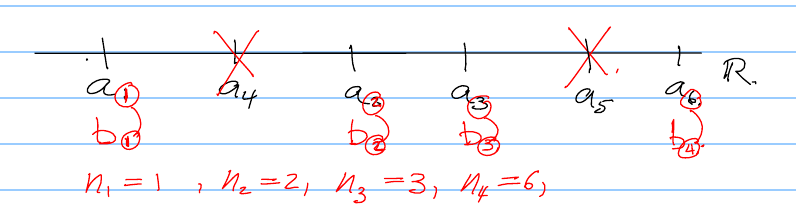
\includegraphics[scale=0.75]{illustrations_Analyse/b_w}
\begin{boite}
\underline{Théorème :} B.W. De toute suite bornée, on peut extraire une sous-suite convergente.
\end{boite}
\underline{Exemple :} $a_n = (-1)^n\\
a_n \in [-2,2]$, donc $(a_n)$ bornée\\
$b_k = a_{\underbrace{2k}_{n_k}} = (-1)^{2k} = 1$\\
$c_k = a_{2k+1} =(-1)^{2k+1} = -1$\\
Donc $\limite{k \to \infty} b_k = 1$ et $\limite{k\to \infty} c_k = -1$ mais $\limite{\ninf} a_n$ n'existe pas.\\
\underline{Explication :}\\
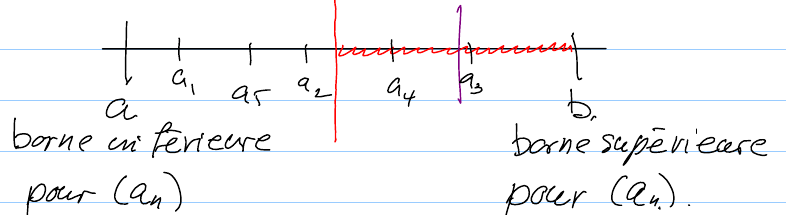
\includegraphics[scale=0.5]{illustrations_Analyse/expli}\\
On divise par deux l'intervalle [a,b] qui contient tous les $(a_n)$ et on retient une moitié qui contient un nombre infini des $a_n$. Puis on recommence. Par récurrence on détermine l'existence d'une limite
\subsection{Limites inférieurs et limite supérieure d'une suite $a_n$ bornée}
\begin{boite}
\Definition : $a\in \R$ est un point d'accumulation de $(a_n)$ s'il existe une sous-suite $(b_k)$ telle que $\limite{k \to \infty} b_k =a$
\end{boite}

\begin{boite}
$E_1 = \{a_1,...\} \inf(E_1) = b_1, \sup(E_1) = c_1$\\
$E_2 = \{a_2,...\} \inf(E_2) = b_2, \sup(E_2) = c_2$\\
$E_3 = \{a_n,...\} \inf(E_n) = b_n, \sup(E_n) = c_n$\\
$(b_n)$ une suite croissante et bornée\\
$(c_n)$ une suite décroissante et bornée\\
$\Rightarrow b := \limite{\ninf} b_n =: \liminf\limits_{\ninf} a_n$\\
$\Rightarrow c := \limite{\ninf} c_n =: \limsup\limits_{\ninf} a_n$\\
\end{boite}
\begin{boite}
\underline{Remarque} : Si $\limsup\limits_{\ninf} a_n = \liminf\limits_{\ninf} = a$ alors 
\begin{equation}
\limite{\ninf} a_n =a
\end{equation}
\end{boite}
\section{Séries numériques}
\setcounter{equation}{0}
\subsection{Définition}
On aimerait définir des "sommes infinies" $\skinf a_k$, pour $a_k \in \R$, c'est à dire pour $(a_k)$ une suite donnée. \underline{Une telle somme infinie est appelée une série numérique}.
\begin{boite}
\Definition : $\skinf a_k := \limite{\ninf} s_n, s_n = \sum^n_{k=0}$
\end{boite}
Donc : $s_0 =a_0\\
s_1 = a_0 + a_1 = s_0 + a_1\\
s_2 = a_0 + a_1 + a_2 = s_1 + a_2$\\
\\
\underline{Terminologie} 
\begin{itemize}
\item les $a_n$ sont appelés les termes de la "somme infinie"
\item La somme finie $s_n$ est appelée n-ième somme partielle de la somme infinie.
\end{itemize}
\underline{Exemple :} $\skinf \frac{1}{2^k} := \limite{\ninf}\underbrace{\sum^n_{k=0} (\frac{1}{2})^k}_{=s_n} = \limite{\ninf}\frac{1-(\frac{1}{2})^{n+1}}{1-\frac{1}{2}} = 2$
\begin{boite}
\Definition : une \underline{série} numérique est dite convergente si la suite $(s_n)$des sommes partielles converge. La limite $s= \limite{\ninf} s_n$ est appelée la \underline{somme} de la série
\end{boite}
\begin{boite}
\Definition : une série $\skinf a_n$ est \underline{absolument} convergente si la série
$\skinf |a_k|$ converge
\end{boite}
\underline{Remarques :}
\begin{itemize}
\item toute série absolument convergente est convergente
\item La somme dune série absolument convergente ne dépend pas de la numérotation de ses termes.
\end{itemize}
\subsection{Exemples}
\subsubsection{La série harmonique}
\begin{boite}[0.5]
$(S=) \sum^\infty_{k=1} \underbrace{\frac{1}{k}}_{a_k}$ cette série diverge
\end{boite}
$\limite{\ninf} s_n = \infty$ (la limite n'existe pas)\\
\underline{Démonstration} (raisonnement par l'absurde)\\
$s_n = \sum^n_{k=1} \frac{1}{k}, b_n = s_{2n} = \sum^{2n}_{k=1} \frac{1}{k}$\\
Supposons que $\underbrace{\limite{\ninf} s_n = s \in  \R}_{\mbox{Hypothèse}} \Rightarrow \limite{\ninf} b_n \underbrace{=}_{\mathclap{\mbox{par définition de la limite}}} s$\\
Alors $b_n-s_n = \sum^{2n}_{k = n+1} \frac{1}{k} \geq \sum^{2n}_{k=n+1} \frac{1}{2n}$
\subsubsection{La série harmonique alternée}
\begin{equation}
S= \somme{\infty}{k=1}(-1)^{k-1}\frac{1}{k} (=ln 2), (-1)^0 = 1
\end{equation}
\begin{itemize}
	\item La série converge, mais pas absolument.
\end{itemize}
\subsubsection{La série géométrique}
\begin{equation}
S = \somme{\infty}{k=0}q^k, q \in \R
\end{equation}
\begin{itemize}
	\item La série géométrique converge absolument pour $0 \leq |q| < 1$
	\item La série géométrique diverge pour $|q| \geq 1$
\end{itemize}
\evid{Démonstration}\\
\begin{equation}
s_n = \somme{n}{k=0}q^k = \frac{1-q^{n+1}}{1-q}	
\end{equation}
si $|q| < 1, n \to \infty$ alors
\begin{equation}
\frac{1}{1-q}
\end{equation}
\subsection{Critères de convergence}
\subsubsection{Critère nécessaire}
\begin{boite}[0.6]
\begin{center}
$\somme{\infty}{k=1}a_k$ converge $ \to \limite{k\to \infty}a_k = 0$\\
$\Leftrightarrow$\\
$\limite{k\to\infty}\neq 0 \to \somme{\infty}{k=1}$ ne converge \underline{pas}
\end{center}
\end{boite}
\evid{Démonstration}\\
Si la série numérique converge, la suite $s_n = \somme{n}{k=0}a_k$ est une suite de Cauchy. Cela veut dire que $\forall \epsilon > 0, \exists n_0$ tel que $\forall n,m\geq n_0, |s_n-s_m|<\epsilon$. En particulier $|s_n - s_{n-1}| < \epsilon$. Mais si $|s_n - s_{n-1}| = a_n$, alors $|a_n| < \epsilon.$ On a donc que $\forall \epsilon > 0$ il existe $n_0$ tel que $|a_n - 0| < \epsilon \Leftrightarrow \limite{\ninf}a_n = 0$
\subsubsection{Critère de Leibnitz}
Si $(a_k)$ est une suite alternée ($(-1)^{k-1}a_k\geq 0$ ou $\leq 0$ pour tout k). Si$(|a_k|)$ est strictement décroissante ($|a_{k+1} < |a_k| \forall k)$ et si $\limite{k\to\infty}a_k =0$, alors la série converge.\\
\evid{Exemple}
\begin{equation}
\somme{\infty}{k=1}(-1)^{k-1}\frac{1}{k}, a_k = \frac{1}{k}
\end{equation}
Les 3 critères sont donc à respecter pour que ce soit une suite de Leibnitz :
\begin{itemize}
	\item La suite doit être alternée
	\item $|a_k|$ doit être strictement décroissant
	\item $|a_k|$ doit tendre vers 0
\end{itemize}

\subsubsection{Critère de comparaison}
\begin{boite}
\begin{itemize}
	\item Si $(0 \leq) |a_k| \leq b_k \forall k$ et si $\somme{\infty}{k=1}b_k$  converge, alors $\somme{\infty}{k=1}a_k$ converge (absolument)
	\item si $0 \leq b_l \leq a_k$ et si $\somme{\infty}{k=1}b_k$ diverge, alors $\somme{\infty}{k=1}a_k$ diverge.
\end{itemize}
\end{boite}
\subsubsection{Critère de d'Alembert et de Cauchy}
\begin{boite}
\Theoreme Si \begin{equation}
\limite{k \to \infty} \left|\frac{a_{k+1}}{a_k}\right| = q \mbox{ existe (d'Alembert)}
\end{equation}
ou si 
\begin{equation}
\limite{k\to\infty}|a_k|^{\frac{1}{k}} \mbox{ existe (Cauchy)}
\end{equation}
Alors
\begin{itemize}
	\item si $0\leq q < 1$ La série converge
	\item si $q \geq 1$ La série diverge
	\item si q = 1, pas de conclusion par cette méthode
\end{itemize}
\end{boite}
\evid{Remarque}Les deux méthodes donnent la même valeur pour q.
[trou exemple]
\subsection{Série avec paramètres}
\begin{enumerate}
	\item Soit la série 
		\begin{equation}
			s = \somme{\infty}{k=1}\frac{k^2}{b^k}, b \neq 0\mbox{ un paramètre}
		\end{equation}
		La converge dépend du choix de b. Selon d'Alembert, 
		\begin{equation}
		\limite{k\to \infty}\left| \frac{\frac{(k+1)^2}{b^{k + 1}}}{\frac{k^2}{b^k}} \right| =  \limite{k\to\infty}\left| \frac{(k+1)^2}{bk^2} \right| = \frac{1}{b} = q
		\end{equation}
		\begin{itemize}
			\item La série converge absolument pour $|b| > 1$
			\item La série diverge pour $0 < |b| < 1$
			\item Le critère ne s'applique pas pour $b = \pm 1$.\\
			Dans ce cas, on a $\somme{\infty}{k=1}k^2$ ou $\somme{\infty}{k=1}(-1)^kk^2$. 
			Ces séries divergent par les critères des sections précédentes.
		\end{itemize}
	\item Soit la série $s = \sum_{k=0}^{\infty} \frac{1}{k!} x^k, x \in \mathbb{R}$. Selon d'Alembert, \\ $\lim_{k \rightarrow \infty} \left| \frac{ \frac{1}{(k+1)!} x^{k+1} }{\frac{1}{k!} x^k} \right| = \lim_{k \rightarrow \infty} \left| \frac{x}{k+1} \right| = 0 = q$\\
		La série converge donc pour tout x. 
\end{enumerate}
\section{Fonctions réelles d'une variable réelle}
\setcounter{equation}{0}
\subsection{Terminologie, conventions}
Nous considérons des fonctions $f:\rtor, x \to y = f(x)$ pour $x \in D(f) \subset \R$ le domaine de définition de $f$\\
\evid{Convention :}\\
En pratique, une fonction est souvent donnée par une expression (une formule, par exemple $f(x) = x^2)$. Alors, il est entendu que le domaine de définition que $D(f)$ soit le plus grand sous-ensemble de \R sur lequel l'expression est bien définie.\\
\evid{Exemples}\\
$f(x) = \sin(x) \iff \begin{array}{l}
f:\rtor, D(f)	 = \R\\
x \to y = \sin(x)
\end{array}\\
f(x) = \frac{2}{1-x^2} \iff \begin{array}{l}
f:\rtor, D(f) = \R\setminus\{-1,1\}\\
x\to y = \frac{2}{1-x^2}
\end{array}$
\subsubsection{Fonctions polynômes}
\begin{equation}
	f(x) = \somme{n}{k = 0}a_k x^k, a_k \in \R, D(f) = \R
\end{equation}

\subsubsection{Fonctions rationnelles}
\begin{equation}
f(x) = \frac{p(x)}{q(x)}, \mbox{ p,q, des fonctions polynômes}\\
D(f) = \R\setminus\{x : q(x) = 0\}
\end{equation}

\subsubsection{Fonctions algébriques}
Fonctions construites à partir de fonctions polynômes et un nombre fini d'opérations $+,-,\cdot,/,\sqrt[n]{}$

\subsubsection{Fonctions transcendantes}
Toutes les fonctions qui ne sont pas algébriques.\\
\evid{Par exemple :} $\sin(x), \ln(x), e^x, \cos(x), \ldots$

\subsection{Définitions}
\begin{boite}
\evid{Croissant} une fonction $f:\rtor$ est \textit{croissante} si $x_1 \leq x_2 \to f(x_1) \leq f(x_2)$ pour tout $x_1,x_2 \in D(f)$. Elle est \textit{strictement croissante} si $x_1 < x_2 \to f(x_1) < f(x_2)$ 
\end{boite}
\begin{boite}
\evid{Décroissant}une fonction $f:\rtor$ est \textit{décroissante} si $x_1 \geq x_2 \to f(x_1) \geq f(x_2)$ pour tout $x_1,x_2 \in D(f)$. Elle est \textit{strictement décroissante} si $x_1 > x_2 \to f(x_1) > f(x_2)$ 
\end{boite}
\begin{boite}
\evid{Monotone} Une fonction est \textit{monotone} si elle est soit croissante soit décroissante.
\end{boite}
\begin{boite}
\evid{Symétrique} Un ensemble est \textit{symétrique} (par rapport à 0) si $x \in \X \to -x \in \X \forall x \in \X$.\\
\underline{Exemples :} $[-1,2]$ et $[-2,1]$ ne sont pas symétriques, alors que $[-3,3]$ et $[-2,1]\cup[1,2]$ le sont.
\end{boite}
\begin{boite}
\evid{Paire} Une fonction $f:\rtor$ est \textit{paire} si $D(f)$ est symétrique et si $f(x) = f(-x) \forall x \in D(f)$\\
\underline{Exemples :}	$0,1,x^2, \cos{x}\frac{e^x+e^{-x}}{2},...$
\end{boite}
\begin{boite}
\evid{Impaire} Une fonction $f:\rtor$ est \textit{impaire} si $D(f)$ est symétrique et si $f(-x) =-f(x) \forall x \in D(f)$\\
\underline{Exemples :} $0,x,x^3\sin(x), \frac{e^x-e^{-x}}{2} $
\end{boite}
\begin{boite}
\evid{Périodique} Une fonction $f:\rtor$ est appelée \textit{périodique} de période $\mathbf{T} > 0$ si$D(f) = \R$ et si $f(x+\mathbf{T}) = f(x), \forall x \in \R$. Le plus petit $\mathbf{T} > 0$ tel que les conditions sont respectées est appelé \underline{la} \textit{période} de $f$\\
\underline{Exemple :} la fonction $\sin^2(x)$ est $2\pi$ périodique, mais la période est de $\pi$
\end{boite}
\subsection{Les fonctions $\sinh$ et $\cosh$}
\evid{Remarque} Soit $f:\rtor$ avec $D(f)$ symétrique. Alors $f =  f_+ + f_-$, avec $f_+$ une fonction paire, et $f_-$ une fonction impaire. On a
\begin{align*}
	f_+(x) = \frac{1}{2}(f(x) + f(-x))\\
	f_-(x) = \frac{1}{2}(f(x)-f(-x))
\end{align*}
\underline{Exemple :} $f(x) = e^x$
\begin{align*}
	e^x = \cosh(x) + \sinh(x)\\
	\cosh(x) = \frac{1}{2}(e^x+e^{-x}\\
	\sinh(x) = \frac{1}{2}(e^x-e^{-x}\\
\end{align*}
\begin{boite}[0.3]
	$\cosh^2(x)-\sinh^2(x) = 1$
\end{boite}
\subsection{Opérations algébriques}
\subsubsection{Fonctions avec parité}
Soient $p_1,p_2,p_3$ des fonctions paires, et $i_1,i_2,i_3$ des fonctions impaires définies sur un domaine symétrique $D, f:\rtor$.\\
Alors :
\begin{itemize}
	\item $p_1+p_2$ est pair
	\item $p_1\cdotp_2$ est pair
	\item $i_1+i_2$ est impair
	\item $i_1\cdot i_2$ est \textbf{pair}
	\item $p\cdot i$ est impair
	\item $i_1 \circ i_2$ est impair ,$\Im(i_2) \in D(i_1)$
	\item $f\circ p$ est pair, $\Im(p) \in D(f)$
	\item $p \circ 1$ est pair, $\Im(i) \in D$
\end{itemize}
\underline{Vérification-Exemple :} $(i_1\circ i_2)(-x) = i_1(1_2(-x)) = i_1(-i_2(x)) = -i_1(i_2(x) = -(i_1\circ i_2)(x)$\\
\evid{Exemples:}\\
\underline{Fonction pairs} $\cos(x) + x^2, \sin(x^2), \cos(\sin(x)), \exp(\cosh(x))$\\
\underline{Fonction impairs} $\sin(x) + x, \sin(x^3),  \sin(\sinh(x)), \sin^3(x)$
\subsubsection{Fonctions périodiques}
Soient $f,g$ ds fonctions périodiques de période $T_f$ et $T_g$ $T_f,T_g > 0), h : \rtor$, Alors 
\begin{boite}
	$\left.
	\begin{array}{l}
	f+g\\
	f\cdot g
	\end{array}
	\right\}$ est T-périodique$ \iff \frac{T_f}{T_g} \in \Q$\\
	$h\circ f$ est $T_f$ périodique
\end{boite} 
\evid{Remarque} $\frac{T_f}{T_g} \in \Q \to \frac{T_f}{T_g} = \frac{r}{s}, r,s \in \N*$\\
\begin{boite}[0.3]
	$T = T_f \cdot s = T_g \cdot r$
\end{boite}
\evid{Attention} Même si $T_f$ et $T_g$ sont \underline{la} période de f et g, T n'est typiquement pas la période de f+g ou $f\cdot g$, et $T_f$ n'est typiquement pas \underline{la} période de $h\circ f)$
\subsection{Exemples}
\begin{enumerate}
\item $f(x) = \frac{x^3cos(x)}{x+tan(x)}$ \\
	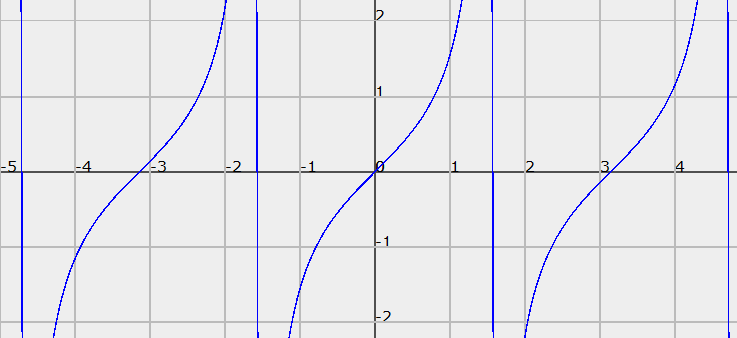
\includegraphics[scale=0.3]{illustrations_Analyse/tanx}\\
	$\mathbf{D}(\tan) = \R\setminus \{\frac{\pi}{2} + n\cdot \pi, n \in \Z\}$
	\begin{itemize}
		\item la fonction est paire
		\item f n'est pas périodique
	\end{itemize}
	
\item $\frac{sin(3x)}{cos(5x)}, \mathbf{D}(f)=\{x \in \R : \cos(5x) \neq 0\} $\\
	\underline{la} période de cos(x) est de $2\pi \to $la période de cos(5x) est de $\frac{2\pi}{5} = T_f$\\
		\underline{la} période de sin(3x) est de $\frac{2\pi}{3} = T_g$\\
		on a $\frac{\frac{2\pi}{5}}{\frac{2\pi}{3}} = \frac{3}{5} \in \mathbb{Q} \to$ f est périodique de $\frac{2\pi}{5}\cdot 5 = \frac{2\pi}{3} \cdot 3 = 2\pi$
		\begin{itemize}
			\item f est une fonction impaire
			\item Après inspection du graph, on trouve que la période est de $\pi$
		\end{itemize}
		
	\item $f(x) = -\overbrace{\sin(\pi \cdot x)}^{\mathclap{\mbox{la période est de 2}}}+\underbrace{\cos(x)}_{\mathclap{\mbox{la période est de }2\pi}}$
		\begin{itemize}
			\item fonction pas périodique, car $\frac{2\pi}{2} \not \in \mathbb{Q}$
			\item f n'a pas de parité
		\end{itemize}
	\item $f(x) = \overbrace{\sin(\tan(x))}^{\mathclap{\mbox{Définie sur le domaine de } \tan(x)}}-\underbrace{\tan(\sin(x))}_{\mathclap{\mbox{Bien définie sur }x\in \R}}$
		\begin{itemize}
			\item période de $2\pi$
			\item impaire
		\end{itemize}
\end{enumerate}

%\subsection{Fonctions définies par étapes}
\subsubsection{Composition (un exemple)}
$f(x)=
\left\{
	\begin{array}{lll}
	x & \mbox{pour} & x > 1\\
	-x & \mbox{pour} &  x<1
	\end{array}
\right.
$\\
\\
$g(x)=
\left\{
	\begin{array}{lll}
	x^2 & \mbox{pour} & x \geq 0\\
	2x+3 & \mbox{pour} &  x<0
	\end{array}
\right.
$\\
\\
$h(x)= (f\circ g)(x) = f(g(x)) =
\left\{
	\begin{array}{cll}
	x^2 & \mbox{pour} & x \geq 1\\
	-x^2 & \mbox{pour} &  0 \leq x < 1\\
	2x+3 & \mbox{pour} & -1 \geq x < 0\\
	-(2x+3) & \mbox{pour} & x < 1
	\end{array}
\right.
$

\subsubsection{Les fonction signum et Heaviside}
sign$(x)=
\left\{
	\begin{array}{lll}
	+1 & \mbox{pour} & x > 0\\
	0 & \mbox{pour} & x = 0\\
	-1& \mbox{pour} & x < 0
	\end{array}
\right.$

$H(x)=
\left\{
	\begin{array}{lll}
	+1 & \mbox{pour} & x > 0\\
	0 & \mbox{pour} & x \leq 0
	\end{array}
\right.$
\subsection{Transformation affines (rappel, voir les pré-requis)}
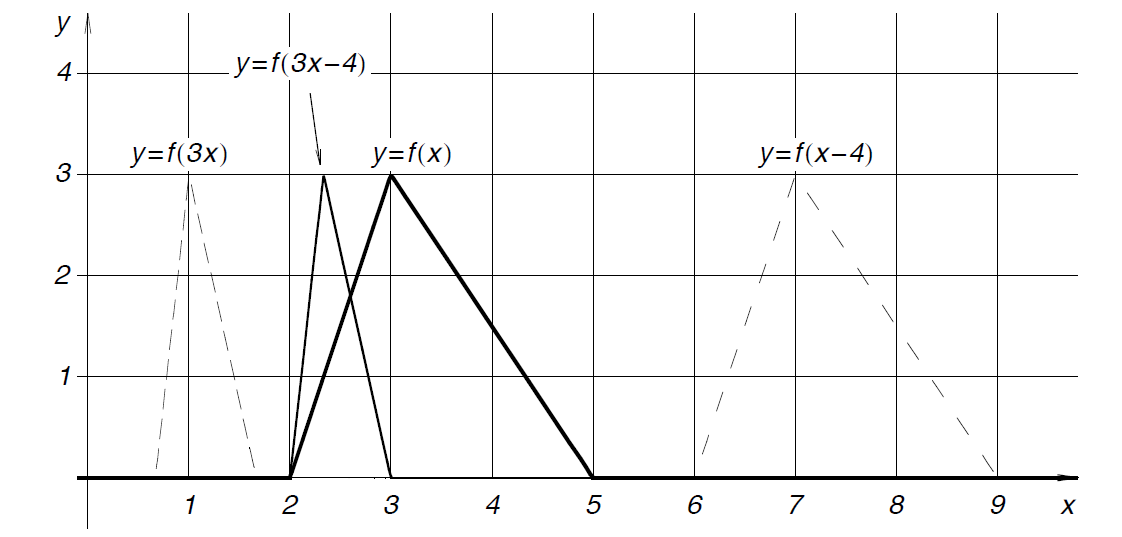
\includegraphics[scale=0.3]{illustrations_Analyse/Affine}\\
$f(3x-4)\equiv \textcolor{red}{f(3x)-4) \equiv g(3x) \to g(x) = f(x-4)}$\\
$f(3x-4) \equiv \textcolor{blue}{f(3(x-\frac{4}{3})) = h(x-\frac{4}{3}) \to h(x) = f(3x)}$
\subsection{Limites}
\subsubsection{Définitions}
Dans ce chapitre, $f: \R \to \R \mbox{ et } \mathbf{D}(f) \subset ]a,b[, a,b \in  \R, a < b$
Soit ($x_n)_{n\geq 1}$ une suite telle que $x_n \in \mathbf{D}(f)$ et supposons que $\limite{\ninf} x_n = x^* \in  ]a,b[$\\
\\
\evid{Question :} Que peut-on dire de la suite $(y_n)_{n\geq 1}$ où $y_n = f(x)$ pour $f$ quelconque ?\\
\evid{Réponse :} Rien du tout : Donnés $(x_n)$ et $(y_n)$ on peut trouver une fonction telle que $f(x_n) = y_n$ (on définit f de cette manière).
\begin{enumerate}
	\item 
\begin{center}
\framecolorbox{red}{white}{\begin{minipage}{0.9\textwidth}
\underline{Définition }(limite épointée)\\
La fonction $f:\rtor$ admet pour limite (épointée) $l \in \R$ lorsque x tend vers $x^*$. Si pour toute suite $(x_n), x_n \in \mathbf{D}(f) \setminus \{x^*\}$ tel que $\limite{\ninf} x_n = x^{*}$. La suite $(y_n), y_n = f(x_n)$ converge et $\limite{\ninf} y_n = l (\iff$ la même limite pour toutes les suites admises) 
\end{minipage}}
\end{center}

	\item
		\begin{center}
			\framecolorbox{red}{white}{
				\begin{minipage}{0.9\textwidth}
				\underline{Définition }(limite du doc de référence)\\
	La fonction $f:\rtor$ admet pour limite $l \in \R$ lorsque x tend vers $x^*$. Si pour toute suite $(x_n), x_n \in \mathbf{D}(f)$ tel que $\limite{\ninf} x_n = x^{*}$. La suite $(y_n), y_n = f(x_n)$ converge et $\limite{\ninf} y_n = l (\iff$ la même limite pour toutes les suites admises) 
		\end{minipage}
		}
	\end{center}
\end{enumerate}

\begin{boite}
\underline{Remarques importantes}
	\begin{enumerate}
		\item Si $x^* \not \in \mathbf{D}(f)$, les deux définitions coïncident
		\item Si $x^* \in \mathbf{D}(f)$
			\begin{itemize}
				\item la limite dans 1. (la valeur de n) peut être différente de $f(x^*)$ car on ne regarde jamais la valeur de $f(x^*)$ dans le calcul de l
				\item On a l = $f(x^*)$ dans 2. (si la limite existe) car $(x_n)$ avec $x_n = x^*$ pour tout n est une suite admise dans 2. (mais pas dans 1.)
			\end{itemize}
	\end{enumerate}
\end{boite}

\underline{Notations :}
\begin{boite}
	\begin{enumerate}
		\item $\limite{\ninf} f(x) \equiv \underset{x \neq x^*}{\lim\limits_{x \to x^*}} f(x) = l$ Limite épointée
		\item $\limite{\ninf} f(x) = l$ Limite selon le document de référence.
	\end{enumerate}
\end{boite}

\underline{Remarques} (au cas ou $x^* \in \mathbf{D}(f)$\\
\begin{itemize}
\item Il se peut que 1. existe mais pas 2 \\
\underline{ex:}
$\left\{
\begin{array}{lll}
0 & \mbox{pour} & x \neq 0\\
1 & \mbox{pour} & x = 0
\end{array}
\right.$
\begin{enumerate}
\item $\underset{x \neq x^*}{\lim\limits_{x \to x^*}} f(x) = 0$
\item $\limite{\ninf} f(x)$ n'existe pas
\end{enumerate}
\item Il se peut que 2 existe mais pas 1
\underline{ex:} $f:[0,0] \to \R, f(0) = 1$
\begin{enumerate}
\item $\underset{x \neq x^*}{\lim\limits_{x \to x^*}} f(x)$ n'existe pas
\item $\limite{\ninf} f(x) = 1$
\end{enumerate}
\end{itemize}

\underline{Exemple :} (avec $x \not \in \mathbf{D}(f)$
\begin{enumerate}
\item f(x) = $\frac{p(x)}{q(x)}, p(x) = x^2+2x+1, q(x) = x+1$\\
$\mathbf{D}(f) = \R \setminus \{-1\},$ on choisit $x^* = -1$\\
$\underset{x \neq -1}{\lim\limits_{x \to -1}} f(x) = \underset{x \neq -1}{\lim\limits_{x \to -1}} \frac{x^2+2x+1}{x+1} = \underset{x \neq -1}{\lim\limits_{x \to -1}} \frac{(x+1)^2}{x+1} = \underset{x \neq -1}{\lim\limits_{x \to -1}} (x+1) \underbrace{=}_{\mbox{Def}} \limite{\ninf} (x_n+1)$ \textcolor{red}{Il faut contrôler toutes les suites $(x_n)$ telles que $x_n \neq -1,\limite{\ninf} x_n = -1$}\\
=$(\limite{\ninf} x_n) +1 = 0$
\item \underline{Non-existence d'une limite}\\
$f(x) = \sin(\frac{1}{x}), \mathbf{D}(f) = \R\setminus\{0\}$\\
Soit $x^* = 0$\\
$\underset{x \neq 0}{\lim\limits_{x \to 0}} f(x)$ n'existe pas. Pour montrer cela :
\begin{itemize}
\item Il suffit de trouver \underline{une} suite $(x_n)$ telle que $x_n \neq x^*$ et $ \limite{\ninf} x_n = x^*$ mais telle que $\limite{\ninf}f(x_n)$ n'existe pas.\\
ou
\item  on trouve \underline{deux} suites$(x_n)$ et $\overset{\sim}{x_n}$ telles que $x_n \neq x^*, \overset{\sim}{x_n} \neq x^*, \limite{\ninf} f(x_n) = l \limite{\ninf} \overset{\sim}{x_n} = \overset{\sim}{l}$
[trou mika, jusqu'aux 2 graphiques concentrés]
\end{itemize}
\end{enumerate}
\subsubsection{Limites}


\begin{boite}
\underline{Définition :} Une fonction $f: \rtor$ admet pour limite à droite (à gauche) $l_+ \in \R (l_- \in \R)$ lorsque q tend vers $x^*$, si pour toue suite $(x_n), x_n \in \mathbf{D}(f) telle que x_n > x^* (x_n < x^*)$. La suite $(y_n), y_n = f(x_n)$ converge et $\limite{\ninf} y_n = l_+ (\limite{\ninf} y_n = l_-)$.
\end{boite}

\underline{Notations}\\
$\ulcorner \limite{x\to x^*+} f(x)\lrcorner \equiv \underset{x > x^*}{\limite{x\to x^*}} f(x) = l_+$\\
$\ulcorner \limite{x\to x^*-} f(x)\lrcorner \equiv \underset{x < x^*}{\limite{x\to x^*}} f(x) = l_-$\\
petit trou\\
\underline{Exemple :} $f(x) = \frac{|x|}{x}. \underset{x\neq 0}{\limite{x \to 0}}$ n'existe pas. $\underset{x > 0}{\limite{x \to 0}}cf(x) = 1, \underset{x < 0}{\limite{x \to 0}}cf(x) = -1$ et -1 $\neq$ 1
\subsubsection{Opérations algébriques sur les limites}
Si\begin{tabular}{c}
$\lim$ \\ 
$x \to x^*$ \\ 
$x \neq x^*$ \\ 
$x > x^*$ \\ 
$x < x^*$ \\ 
\end{tabular} 

[trou mika]\\
\underline{Exemple} $\underset{x \neq 2}{\limite{x \to 2}} (3x^2 -2xx +5) = ... = 3 (\underset{x \neq 2}{\limite{x \to 2}}x)^2 - 2(\underset{x \neq 2}{\limite{x \to 2}}x) + 5 = 3\cdot 2^2 - 2 \cdot 2 + 5 = 3$

\subsubsection{Limites épointées et composition de fonctions}
(attention au piège)
soit 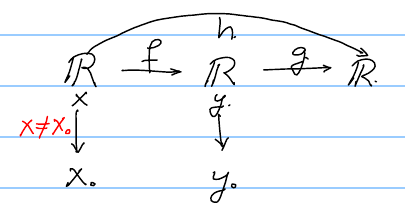
\includegraphics[scale=0.5]{illustrations_Analyse/compo}\\
avec $\underset{x \neq x^*}{\limite{x \to x^*}} f(x )= y^*, \underset{y \neq y^*}{\limite{y \to y^*}} g(x) = l$\\
\underline{Alors (attention aux conditons)}
\begin{boite}
$\underset{x \neq x^*}{\limite{x \to x^*}} h(x) = \underset{x \neq x^*}{\limite{x \to x^*}} g(f(x)) = l$\\
Pourvu que pour toute suite $(x_n), x_n = x^*$ et $\limite{\ninf} x_n = x^*$ il existe un $n_0$ tel que $f(x_n) yequiv y_n \neq y^*$ pour tout $n \geq n_0$
\end{boite}
\underline{Remarque :} Cette difficulté disparaîtra pour f,g des fonctions continues.\\
\underline{Exemple :} $g(x) =
\left\{
\begin{array}{lll}
0 & \pour & x = 1\\
2 & \pour & x \neq 1
\end{array}
\right.\\
f(x) = 1$ pour tout $x \in \R$\\
$g(f(x)) = 0$ pour tout x, mais $\underset{x \neq x^*}{\limite{x \to x^*}} f(x) = 1 = y^*$ et $\underset{y \neq y^*}{\limite{y \to y^*}} g(y) = 2 \neq \underset{x \neq 0}{\limite{x \to 0 = x^*}}$[petit trou]\\
\subsubsection{"Limites infinies" et comportement à $\infty$}
\underline{Conventions :}
\begin{itemize}
\item $\underset{x \neq x^*}{\limite{x \to x^*}} f(x) = +\infty (ou -\infty)$ veut dire que pour toute suite $xn, x_n \in \mathbf{D}(f), x_n \neq x^*m \limite{\ninf} x_n = x^*$ on a 
%\fbox{\begin{minipage}{0.9\textwidth}
%$\limite{\ninf} f(x_n} = + \infty$
%\end{minipage}}
(ou $-\infty)$
\item {encore un trou...}
\end{itemize}
\subsubsection{Théorème des deux gendarmes}
\begin{boite}
\underline{Théorème} soit f,g, des fonctions de $\rtor$ telles que 
\begin{itemize}
\item $\mathbf{D}(h) \subset \mathbf{D}(f) \cap \mathbf{D}(g)$ pour x proche de $x^*$
\item pour x proche de x* 
\begin{equation}
f(x) \leq h() \leq g(x)
\end{equation}
\item f(x) = g(x) = l 
\end{itemize}
Alors h(x) = l
\end{boite}
"x proche de x*" : $\exists \epsilon > 0$ tel que $\forall x \neq x_0$ avec $|x -x^*| < \epsilon$\\
\\
\underline{Démonstration}\\
soit $(x_n)$ une suite dans $\mathbf{D}(h),x_n \neq x^*, \limite{\ninf} x_n = x^*$. Par hypothèse 1 et 2, on a 
\begin{equation}
f(x_n) \leq h(x_n) \leq g(x_n)
\end{equation}
pour n suffisamment grand. En utilisant le point 3. et le théorème des deux gendarmes pour les suites, alors $h(x_n)$ tend vers l
\subsubsection{Exemples}
\begin{enumerate}
\item $\limite{x to \infty} (\sqrt{x^2+x}-x) = \limite{x \to \infty} \frac{x}{\underbrace{\sqrt{x^2+x}+x}_{= h(x)}}$ \\
Sans restriction $x > 0 :$\begin{align*}
h(x) &\leq \frac{x}{\sqrt{x^2}+x} = \frac{1}{2}\\
& \geq \frac{x}{2\sqrt{x^2+x}}=\frac{1}{2} - \frac{\sqrt{x^2+x}-x}{2\sqrt{x^2}+x}\\
& = \frac{1}{2}- \frac{x}{2\underbrace{\sqrt{x^2+x}}_{\geq x}\underbrace{(\sqrt{x^2+x} +x)}_{\geq 2x}} \geq \frac{1}{2}-\frac{1}{4x}\\
\frac{1}{2}&\geq h(x) \geq \underbrace{\frac{1}{2}-\frac{1}{4x}}_{\mathclap{x\to \infty : \frac{1}{2}-\frac{1}{4\infty}= \frac{1}{2}}}
\end{align*} 
Donc $\frac{1}{2} \geq \limite{x \to \infty} h(x) \geq \frac{1}{2}$ et donc $\limite{x\to\infty} h(x) = \frac{1}{2}$

\item \begin{boite}
Reminder : pour $0 \leq x \leq \frac{\pi}{4} \to 0 \leq \sin x \leq x \leq \tan x$
\end{boite}
$\limite{x \to \neq 0} \cos(x) = 1$. Une fonction paire : on peut se limiter à $x > 0$. On va prendre $0 < x < \frac{\pi}{4}$\\
\begin{align*}
1 \geq \cos(x) &= \sqrt{1-\sin(x)^2} \geq \sqrt{1-2\sin(x)^2 + \sin(x)^4}\\
&= 1 - \sin(x)^2 \geq 1-x^2
\end{align*}
Donc $\underbrace{\underbrace{1}_{1} \geq \cos(x) \underbrace{\geq 1-x^2}_{1}}_{1}$\\
Remarque : $\limite{\ninf} \cos(\frac{1}{n})$

\item $\limite{x \to \neq 0} \frac{\sin(x)}{x} = 1; \frac{\sin(x)}{x}$ est une fonction paire.\\
Pour $0 < x < \frac{\pi}{4}$.\\
$0 < \sin(x) \leq x \leq \tan(x) = \frac{\sin(x)}{\cos(x)}$. On multiplie par $\frac{1}{\sin(x)}$\\
$1 \leq \frac{x}{\sin(x)} \leq \frac{1}{\cos(x)} \Leftrightarrow \underbrace{\cos(x)}_{\to 1\mbox{ 
quand x } \to 0} \leq\frac{\sin(x)}{x} \leq 1$

\item $\limite{x \to \neq 0} \frac{1-\cos(x)}{x} = \limite{x \to \geq 0} (\frac{\overbrace{1-\cos(x)^2}^{\sin^2}}{x^2}\cdot \frac{1}{1+\cos(x)} = ((\frac{\sin(x)}{x})^2 \cdot \frac{1}{1+\cos(x)})\\
= 1^2 \cdot \frac{1}{1+1} = \frac{1}{2}$

\item $\limite{\ninf} e^x = \infty\\
\limite{x \to -\infty} e^x = 0$

\item $f(x) = e^{\frac{1}{x}}$\\
$\mathbf{D}(f) = \R^*$\\
$\limite{x \to > 0} e^{\frac{1}{x}} = \limite{y \to \infty}e^y = 0$
\end{enumerate}

\subsubsection{Définition de la limite (épointée) avec $\epsilon$ et $\delta$}
(Définition équivalente à la définition avec les suites)\\
\begin{center}
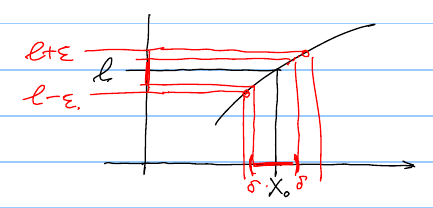
\includegraphics[scale=0.5]{illustrations_Analyse/lim_epoint_epsilon}\\
\end{center}
\begin{boite}
\Definition :La fonction  f: \rtor admet par limite $l \in \R$ lorsque x tend vers $x^*$, si $\forall \epsilon > a, \exists \delta >0$ tel que $|f(x) - l| < \epsilon, \forall x \in \mathbf{D}(f)$ tels que $0 < |x-x^*| < \delta$
\end{boite}
\Exemple : $f(x) = 2x, x^* = 0, \limite{\substack{x \to 0 \\ x \neq 0}} = 0 = l$\\
A montrer : $\forall\epsilon > 0, \exists \delta$ tel que $|2x - 0| < \epsilon$ (ok pour $\delta = \frac{\epsilon}{2})$\\
Car $|2x-0| = |2x| = 2|x| = 2|x-0| \leq 2\delta \leq \epsilon$\\
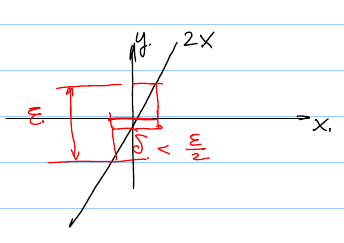
\includegraphics[scale=0.5]{illustrations_Analyse/epsilon2x}

\subsection{Fonctions continues}
\underline{Notation :} A partir de maintenant, on écrira $x_ 0$ au lieu de $x^*$ pour les points qui nous intéressent\\
\begin{boite}
\Definition : La fonction f: \rtor est continue en $x_0 \in \mathbf{D}(f)$ si 

$\limite{\substack{x \to x_0 \\ x \neq x_0}} f(x) = f(x_0) \textcolor{red}{(\Leftrightarrow \limite{x \to x_0} f(x) \mbox{existe})}$
\end{boite}
\subsubsection{Exemple :}
$f(x) = 
\left\{
\begin{array}{lll}
\frac{\sin(x)}{x} & \pour & x \neq 0\\
1 & \pour & x = 0 (\to f(0) 
\end{array}
\right.$
est continu en $x_0 = 0$ car \begin{equation}
\limite{\substack{x\to 0 \\ x \neq 0}} f(x) = \limite{\substack{x\to 0 \\ x \neq 0}} \frac{\sin(x)}{x} = 1 = f(0)
\end{equation}
\ovalbox{f: \rtor} $\supset$ \ovalbox{$\substack{f:\rtor \\ \limite{\substack{x \to x_0\\ x \neq 0}} f(x) = l \in \R}$}$ \supset$\\
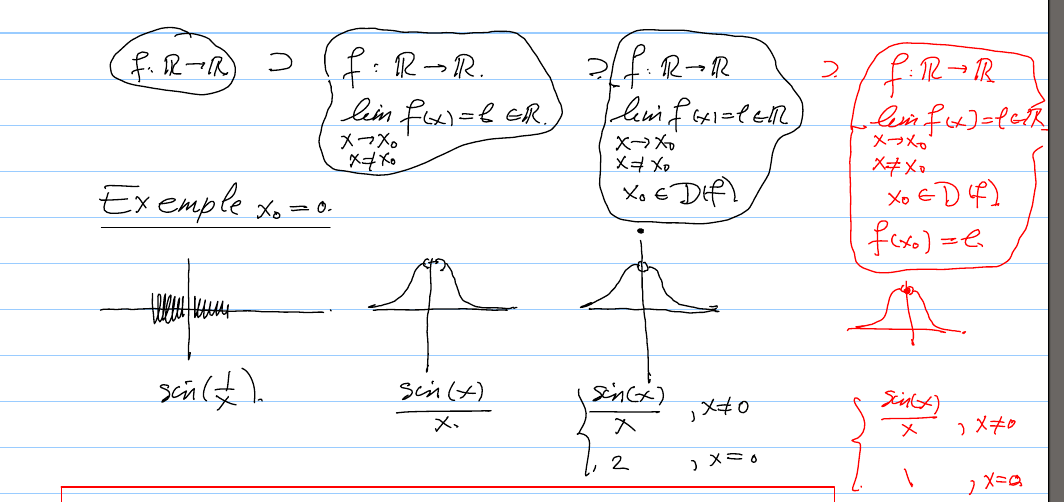
\includegraphics[scale=0.5]{illustrations_Analyse/nakwa}

\begin{boite}
\underline{Remarque :} $\limite{\substack{x \to x_0 \\ x \neq x_0}}f(x) = f(x_o) = f\left(\limite{x \to x_0}x\right)$\\
Si f est continue en $x_0$
\end{boite}

\subsubsection*{Prolongement par continuité}(voir exemple 4.9.1)
Si $\limite{\substack{x \to x_o \\ x \neq 0}} f(x) = l \in  \R$ mais $x_0 \not \in \mathbf{D}(f)$ alors on peut définir une fonction g sur $\mathbf{D}(f) \cup \{x_0\}$ par\\
$g(x) = \left\{
\begin{array}{lll}
f(x) & \pour & x \neq x_0\\
l & \pour& x= x_0
\end{array}
\right.$
Par définition g est continue en $x_0$
\begin{boite}=  
\Definition La fonction $f : \rtor$ est continue sur $I = ]a,b[ \subset \mathbf{D}(f)$ si f est continue en tout point $x_0 \in I$
\end{boite}
\subsubsection{Propriétés des fonctions continues}
\begin{boite}
\Remarque La composition de deux fonctions continues (sur $]a,b[$) est une fonction continue
\end{boite}
\begin{boite}
\Remarque L'image d'une intervalle ouvert par une fonction continue est un intervalle, ais pas forcément ouvert et pas forcément borné
\end{boite}
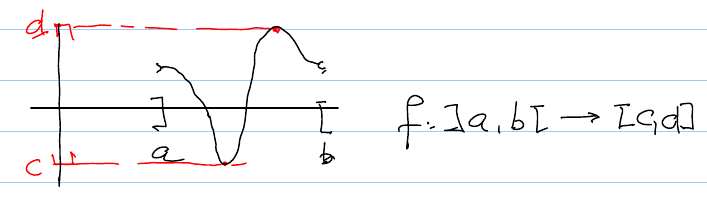
\includegraphics[scale=0.5]{Illustrations_Analyse/interv_ouvert}
\begin{boite}
\Remarque L'image d'un intervalle ouvert par une fonction continue strictement monotone est un intervalle ouvert (éventuellement non-borné)
\end{boite}
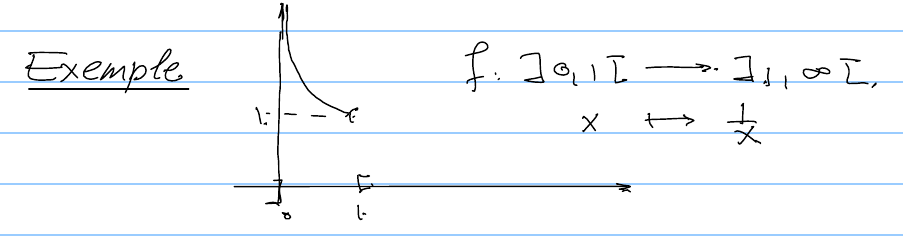
\includegraphics[scale=0.5]{Illustrations_Analyse/interv_mono}
\subsubsection{Fonctions "élémentaires"}

\begin{boite}
\Theoreme : Les fonctions "élémentaires" sont toutes continues sur leur domaine de définition
\end{boite}

\begin{boite}
\underline{Conséquences} pour les fonctions "élémentaires" on a pour $x_0 \in \mathbf{D}(f)$ que $\limite{\substack{x \to x_0 \\ x \neq x_0}} f(x) = f(x_0)$
\end{boite}
\Exemple $\limite{\substack{x \ to x_0 \\ x \neq x_0}} \cos(x) = \cos(0) = 1\\
\limite{\substack{x \ to x_0 \\ x \neq x_0}} \exp(\cos(\ln(\sqrt{\cosh(x)}))) = e\\
\limite{\substack{x \ to x_0 \\ x \neq x_0}} \sin(\frac{1}{x}) = \sin(\frac{1}{x_0}),\forall x_0 \in \mathbf{D}(\sin(\frac{1}{x}) = \R*$
\subsubsection{Intervalles fermés}
\begin{boite}
\Definition La fonction f:\rtor est continue à droite (à gauche) en $x_0 \in I = [a,b[ (]a,b]) \subset \mathbf{D}(f)$ si 
\begin{equation}
\limite{\substack{x \ to x_0 \\ x > x_0}} f(x) = f(x_0) (\limite{\substack{x \ to x_0 \\ x < x_0}} f(x) = f(x_0)
\end{equation}
\end{boite}
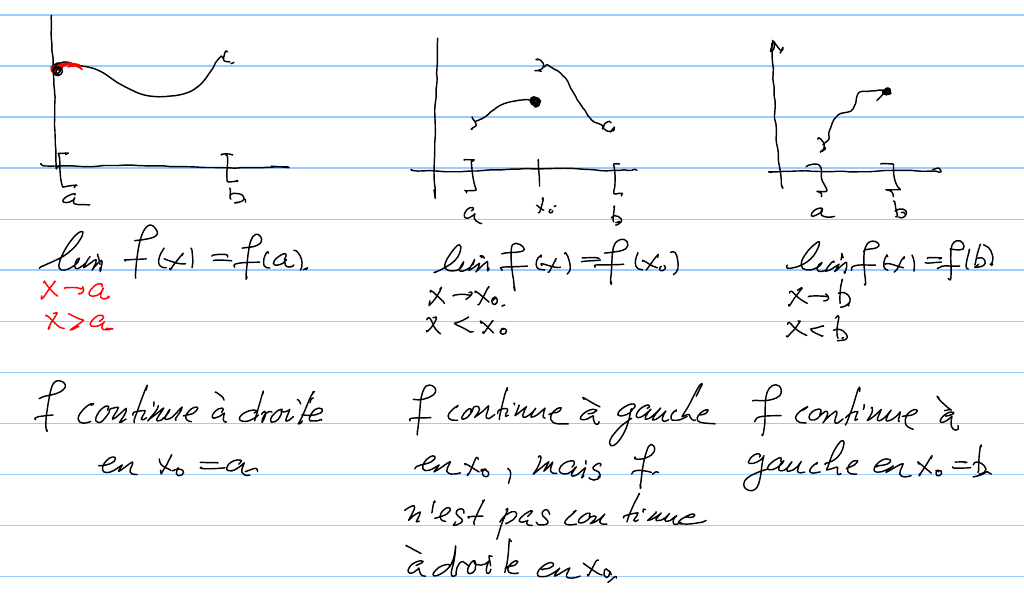
\includegraphics[scale=0.5]{illustrations_Analyse/interv_ferme}

\begin{boite}[0.85]
\begin{tabular}{ll}
\Remarque f continue en \Xo $\Leftrightarrow$ & f continue à droite en \Xo \\
& \underline{et} f continue à gauche en \Xo
\end{tabular}
\end{boite}

\begin{boite}
\Definition La fonction f : \rtor est continue sur $I = [a,b] \subset \mathbf{D}(f)$ si f est continue sur $]a,b[$, continue à droite en $x_0 = a$ et continue à gauche en $x_0 = b$
\end{boite}
\begin{boite}
\Theoreme 1 :; Toute fonction continue $f:[a,b] \to \R$ admet un \underline{maximum} et un \underline{minimum} c'est à dire il existe $c,d \in [a,b]$ tels que $f(c) \leq f(x) \leq f(d)$ pour tout $x \in [a,b]$
\end{boite}

\underline{Démonstration} utilise B.W.\\
\underline{Notation} $\underbrace{m}_{\min} = \substack{\min f(x)\\ x \in [a,b]}, \underbrace{M}_{\max} = \substack{\max f(x)\\ x \in [a,b]}$
\begin{boite}
\Theoreme 3: Soit $f : [a,b] \to \R$ continue sur [a,b]. Alors $Im(f) =[m,M]$
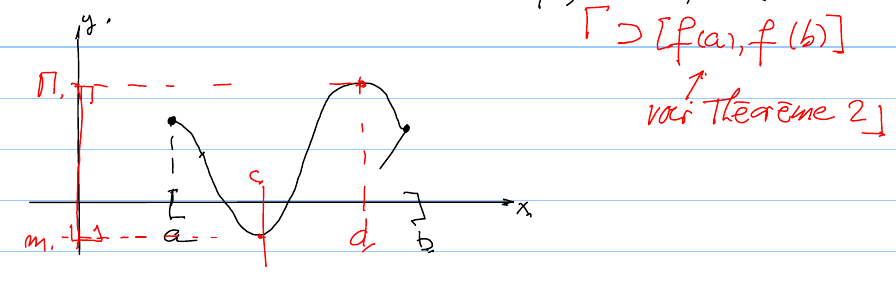
\includegraphics[scale=0.5]{illustrations_Analyse/theo_3}
\end{boite}
\begin{boite}
\Theoreme 2 : (de la valeur intermédiaire) Toute fonction continue $f:[a,b] \to \R$ prend (une fois au moins) toutes les valeurs entre $f(a) et f(b)$\\
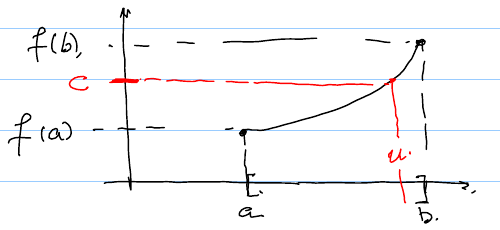
\includegraphics[scale=0.5]{illustrations_Analyse/theo_4}
\end{boite}
\underline{Démonstration} Supposons que $f(a) < f(b)$. On cherche $u \in [a,b]$ tel que $f(u) = c$ pour $c \in [f(a), f(b)]$ pour c donné.\\
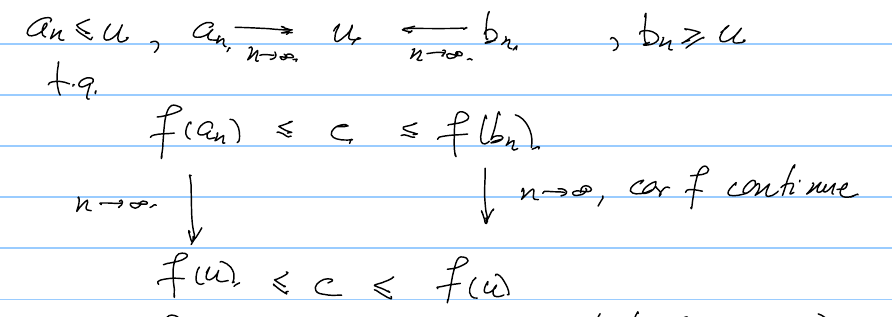
\includegraphics[scale=0.5]{illustrations_Analyse/demo_theo_2} $\to c = f(u)$\\
Les suites $(a_n$) et $(b_n)$ se construisent en appliquant la méthode de bissection à la fonction $g(x) = f(x)-c /\ g(x) = 0 \Leftrightarrow f(x) = c$
\subsubsection*{Méthode de bissection}
Si la fonction $g: [a,b] \to \R$ est continue et si $g(a) < 0$ et $g(b) > 0$, alors il existe $u \in [a,b]$ tel que $g(u) = 0$\\
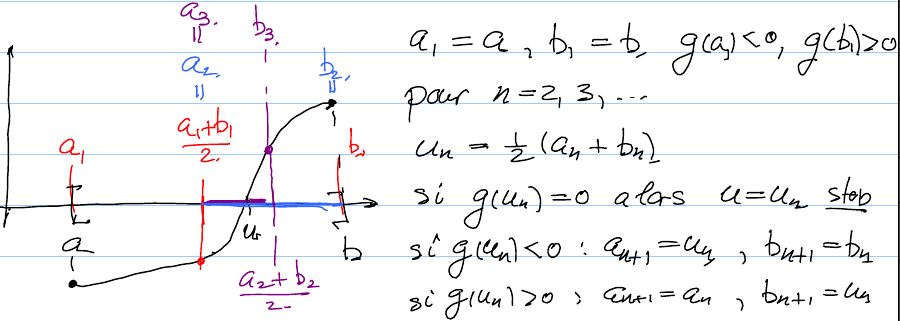
\includegraphics[scale=0.5]{illustrations_Analyse/metho_bissec}\\
\Exemple Soit $g(x) = x^2 -2, g:[1,2] \to \R$ $ g(1) = -1 < 0, g(2) =  > 0$\\
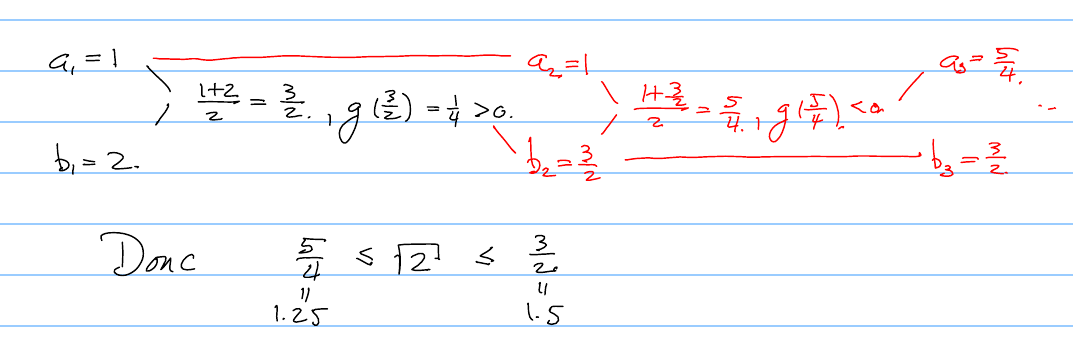
\includegraphics[scale=0.5]{illustrations_Analyse/exemple_bissec}\\
\underline{Avantages :} 
\begin{itemize}
\item la convergence est garantie
\item convergence seulement linéaire
\end{itemize}
On a $u_n \in [a_n, b_n]$, longueur de $[a_n,b_n] = \frac{b-a}{2^n}$\\
On a $\ln(\frac{b-a}{n^2}) = \ln(b-a) - \underbrace{n\cdot \ln(2)}_{\mathclap{\mbox{linéaire en n}}}$\\
(le \# de digits corrects croit linéairement)
\begin{boite}
\Definition la fonction $f: \rtor$ admet un point fixe si l'équation $f(x) = x$ admet une solution
\end{boite}

\begin{boite}
\Theoreme (du point fixe) Toute fonction continue $f:[a,b] \to [a,b]$ admet un point fixe
\end{boite}
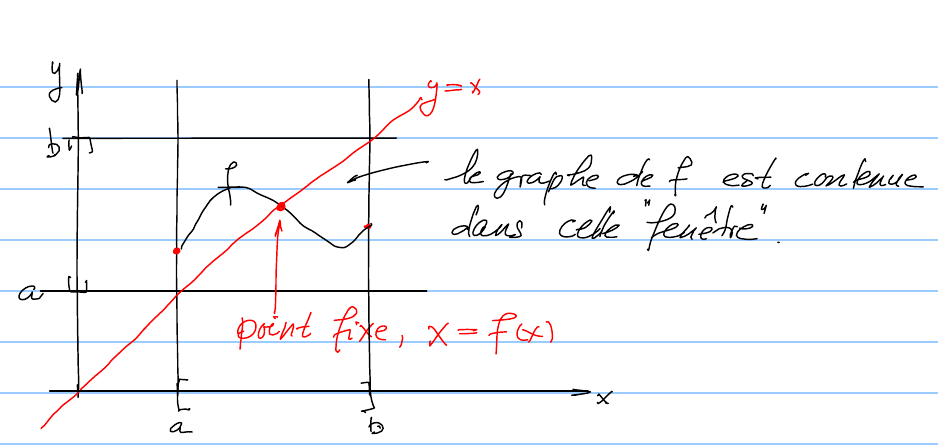
\includegraphics[scale=0.5]{illustrations_Analyse/point_fixe}\\
\underline{Démonstration} appliquer la méthode de bissection à $g(x) = f(x) -x$ (ou $g(x) = x -f(x)$

\section{Dérivée d'une fonction d'une variable}
\setcounter{equation}{0}
Dans ce chapitre $f_ \rtor, x_0 \in ]a,b[ \subset \mathbf{D}(f)$\\
\subsection{Définitions}
\begin{boite}
\Definition (dérivable) La fonction f est dérivable en \Xo, si la limite 
\begin{equation}
\limite{\substack{x\to x_0 \\ x\neq x_0}} \frac{f(x)-f(\Xo)}{x- \Xo} \equiv d_{\Xo} \mbox{ existe}
\end{equation}
\end{boite}
\underline{Nota Bene} $d_{\Xo}$ est un nombre\\
\underline{Remarque :} $\limite{\substack{x\to x_0 \\ x\neq x_0}} \frac{\overbrace{f(x) - f(\Xo)}^{x_0 + h \Leftrightarrow h = x- x_0}}{x-\Xo} =  \limite{\substack{h \to 0 \\ h \neq 0}} \frac{f(x_0 + h) - f(x_0)}{h}$\\
\underline{Remarque} Si f est continue en $x_0 \limite{\substack{x \to x_0 \\ x \neq x_0}} f(x) - f(x_0) = 0$
\begin{center}
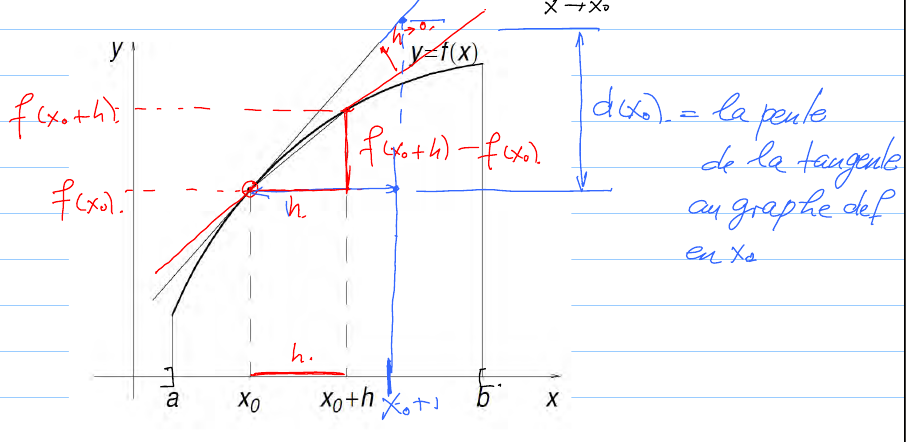
\includegraphics[scale=0.5]{illustrations_Analyse/deriv}
\end{center}
\begin{boite}
\Definition (différentiable) La fonction f est différentiable en $x_0 \in ]a,b[ \to \R$ s'il existe un nombre $\alpha \in \R$ et une fonction $r: ]a,b[ \to \R$ tel que 
\begin{equation}
f(x_0+h) = f(h_0) + \alpha h + \framecolorbox{red}{white}{$r(x_0 + h) \cdot h$}
\end{equation}
avec $\limite{\substack{h \to 0 \\ h \neq 0}} \framecolorbox{red}{white}{$r(x_0 + h) = 0$}$\\
$\iff \limite{\substack{h \to 0 \\ h \neq 0}} \frac{r(x_0 + h) \cdot h}{h} = 0$\\
\framecolorbox{red}{white}{$r(x_0 + h) = 0$} est o(h)
\end{boite}
\evid{Remarque} dérivable $\iff$ différentiable\\
$``\to'' \limite{\substack{h \to 0 \\ h \neq 0}} \frac{f(x_0 + h) - f(x_0)}{h} = d(x_0) =:\alpha$\\
on a\\
$r(x_0 + h)  \frac{f(x_0 + h) - f(x_0) - \alpha h}{h} = \frac{f(x_0 + h) - f(x_0)}{h} - \alpha$\\
Donc\\
$\limite{h \to 0} r(x_0 + h) = d(x_0) - \alpha =| 0$ pour $\alpha = d(x_0)\\
"\leftarrow" on a \frac{f(x_0 + h) - f(x_0)}{h} = \alpha + r(x_0+h)\\
$donc $\limite{\substack{h \to 0 \\ h \neq 0}} \frac{f(x_0 + h) - f(x_0)}{h} = \alpha + \limite{\substack{h \to 0 \\ h \neq 0}} r(x_0 + h) = \alpha$
\begin{boite}
\Definition \\
On dit que f est dérivable (différentiable) sur $]a,b[ \subset D(f)$ si f est dérivable (différentiable) en tout point $x_0 \in ]a,b[$
\end{boite}

\begin{boite}
\Definition \\
Soit la fonction f dérivable sur $]a,b[$. Alors on peut définir la fonction f', appelée la dérivée de f par 
\begin{equation}
f'(x) = dx \equiv \limite{\substack{h \to 0 \\ h \neq 0}} \frac{f(x_0 + h) - f(x_0)}{h}
\end{equation}
\end{boite}

\begin{boite}
\Definition (fonction dérivée d'ordre n)\\ 
Si la fonction $f'$ est dérivable sur $]a,b[$, on peut définir la fonction $f''$ appelée la deuxième dérivée (ou dérivée seconde) de $f$ par $f''(x) = (f')'(x)$ et puis par récurrence, si la (n-1)ème dérivée de la fonction f est dérivable sur $]a,b[$ on peut définir la fonction $f^{(n)}$ (la n-ième dérivée de f) par $f^{(n)}(x) = (f^{(n-1)})'(x), n = 2,3,... $
\end{boite}
\subsection{Exemples (à savoir par coeur}
(Sans démonstration)\\
\begin{center}
$\begin{array}{ccc}
f & f' & f^{(n)} n = 2,...\\
1 & 0 & 0\\
x & 1 & 0\\
x^m & m\cdot x^{m-1} & 
\left\{ \begin{array}{ll}
m(m-1)(m-2)...(m-n+1)x^{m-n} & n \leq m\\
0 & n > m
\end{array} \right.\\
&[trou]&\\
e^x & e^x & e^x\\
\arctan(x) & \frac{1}{1+x^2} & \mbox{pas nécessaire}
\end{array}$
\end{center}
\subsection{Dérivabilité implique continuité}
\begin{boite}
\Theoreme\\
Une fonction qui est $\underbrace{\mbox{dérivable en }x_0}_A$ est $\underbrace{\mbox{continue en }x_0}_B$\\
$A \to B$
\end{boite}
\evid{Démonstration} $\limite{\substack{x \to x_0 \\ x \neq x_0}}(f(x)- f(x_0)) = \limite{\substack{x \to x_0\\ x \neq x_0}}\left(\frac{f(x) - f(x_0)}{x - x_0} (x-x_0)\right)\\
 = \underbrace{\left(\limite{\substack{x \to x_0 \\ x \neq x_0}}\frac{f(x) - f(x_0)}{x-x_0}\right)}_{d(x_0) \in \R}\underbrace{\left(\limite{\substack{x \to x_0 \\ x \neq x_0}}(x-x_0)\right)}_{=0} = 0$\\
\begin{center}
\evid{La réciproque du théorème est fausse !} ($B\not \to A$)
\end{center}
\evid{Contre exemple} $f(x) = |x| = 
\left\{
\begin{array}{lll}
x & \pour & x \geq 0\\
-x & \pour & x < 0
\end{array}
\right.$\\
$x_0 = 0:$ \underline{f est continue en $x_0$}
[TROU]
\subsection{Intervalles fermées}
\begin{boite}
\Definition (voir l'exemple précédent)\\
La fonction $f: \rtor$ est dérivable à droite (à gauche) en $x_0 \in I, I = [a,b[ (]a,b]), \subset D(f)$ si 
\begin{equation}
\limite{\substack{x \to 0 \\ h > 0}} \frac{f(x_0 + H) - f(x_0)}{h} \equiv d_+(x_0) \in \R\mbox{ existe}
\end{equation}
\begin{equation}
\left(\limite{\substack{x \to 0 \\ h < 0}} \frac{f(x_0 + H) - f(x_0)}{h} \equiv d_-(x_0)  \in \R\mbox{ existe}\right)
\end{equation}
\end{boite}
\begin{boite}
\evid{Remarque}\\
f dérivable en $x_0 \in ]a,b[ \iff $f dérivable à droite en $x_0$ et f dérivable à gauche en \Xo et $d_+(x_0) = d_-(x_0) (=d(x_0))$
\end{boite}
\begin{boite}
\Definition
La fonction f:\rtor est dérivable sur $I=[a,b] \subset D(f)$ si f est dérivable sur $]a,b[$, dérivable à droite en a et dérivable à gauche en b
\end{boite}
\begin{boite}
\evid{Exemple} $f(x) = \sqrt{1-x^2}$ est continue sur $[-1,1]$ dérivable sur $]-1,1[$ (mais pas $[-1,1]$)\\
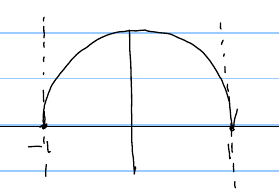
\includegraphics[scale=0.5]{illustrations_Analyse/sqrtx}
\end{boite}
$\limite{substack{h \to 0 \\ h > 0}} \frac{f(-1+h) - f(-1)}{h} = \infty, \limite{\substack{h \to 0 \\ h < 0}} \frac{f(1+h) - f(1)}{h} = -\infty$
\subsection{Opérations algébriques sur les dérivées}
$f,g : \rtor$ dérivable sur $]a,b[ \subset D(f) \cap D(g), \alpha, \beta \in \R$

\begin{boite}
$\begin{array}{ccc}
(\alpha f + \beta g)' & = & \alpha f' + \beta g'\\
(f\cdot g)' & = & f'\cdot g + f\cdot  g'\\
\left(\frac{f}{g}\right)' & = & \frac{f'\cdot g - f\cdot g'}{g^2}
\end{array}$
\end{boite}

\evid{Exemple} $a_k \in \R, k = 0,...n\\
f(x) = \sum^n_{k=0} a_k\cdot x^k = a_0 + a_1\cdot x +...\\
f'(x) = \sum^n_{k=1} a_k\cdot k \cdot x^{k-1} = \sum^{n-1}_{k=0}a_{k+1}(k+1)x^k$
\subsection{Dérivée de la composition de deux fonctions}
$]a,b[ \overset{f}{\to} ]c,d[ \overset{g}{\to}\R$ f dérivable en \Xo, g dérivable en $y_0$
[trou]\\
\begin{boite}
\Theoreme (dérivation en chaine\\
\framecolorbox{red}{white}{$(g\circ f)'(x_0) = (g'\circ f)(x_0) \circ f'(x_0)$}
\end{boite}
\evid{Ceci se généralise par récurrence (exemple)}\\
$f(x) = \cos(\ln(\sqrt{1+x^2})), D(f) = \R\\
f'(x) = -\sin(\ln(\sqrt{1+x^2}))\cdot \frac{1}{\sqrt{1+x^2}} \cdot \frac{1}{2\sqrt{1+x^2}} \cdot 2x$\\
\evid{Démonstration}\\
($(g \circ f)(x_0 + h) = (g \circ f)(x_0) + (g \circ f)' (x_0) h +o(h)$
[trou mika]

\subsection{Continuité de la fonction dérivée}
(Ne pas confondre avec 5.3 !)\\
\evid{Un contre-exemple:} (f n'est pas nécessairement continue)\\
soit $f(x) = 
\left\{
\begin{array}{lll}
x^2\sin(\frac{1}{x}) & \pour & x \neq 0\\
0 & \pour & x = 0
\end{array}
\right.\\
D(f) \in \R$ n'est pas continue sur \R (vérifier !)\\
\\
\evid{f est dérivable sur \R} ($\to$ f est continue sur \R)
\begin{enumerate}[label=\roman*.]
	\item pour $x \neq 0$ on a 
		\begin{equation}
			f'(x) = 2x\sin(\frac{2}{x}) + x^2\cos(\frac{1}{x})\frac{-1}{x^2}
		\end{equation}
	\item Pour $x = 0$ on a (utiliser la définition)
		\begin{equation}
			f'(0) = \limite{\substack{h \to 0 \\ h \neq 0}} \frac{f(0+h) - f(0)}{h} = 
			\limite{\substack{h \to 0 \\ h \neq 0}}\frac{h^2\sin(\frac{1}{h}-0}{h} = \limite{\substack{h \to 0 \\ h \neq 0}} (h \sin(\frac{1}{h})) \underbrace{=}_{\mathclap{\substack{\mbox{Théorème des} \\ \mbox{deux gendarmes}}}} 0
		\end{equation}
\end{enumerate}
Donc $f'(x) = 
\left\{
\begin{array}{lll}
\frac{1}{1}[???]
\end{array}
\right.$\\
D(f') = \r\\
f' n'est pas continue sur \R, car f' n'est pas continue en x = 0.\\
\evid{Démonstration} Soit $x_n = \frac{1}{2\pi n}, n \in \N*$\\
$\limite{\ninf} f'(x_n) = \limite{\ninf} = \limite{\ninf}(\frac{2}{2\pi n}\sin(2\pi n)-\cos(2\pi n)) = -1 \neq 0 = f'(0)$\\
%[deux images]\\
Par contre, 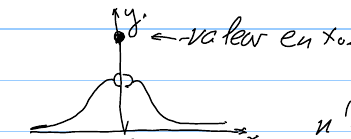
\includegraphics[scale=0.5]{illustrations_Analyse/pas_possible}est pas possible comme dérivée d'une fonction.
\begin{boite}
	\Theoreme : Soit f:\rtor, $x_0 \in ]a,b[ \subset D(f)$. Soit f continue sur $]a,b[$, et dérivable. $[a,b]\setminus\{x_0\}$ et soit $\llimite{x \to x_0}{c \neq x_0}{f'(x)} = l$\\
	Alors f est dérivable en$x_0$ et $f'(x) 
	= l$
\end{boite}
\evid{Attention à la logique} Dans exemple (i),$\llimite{x \to x_0}{x \neq x_0}{ f'(x)}=$ n'existe pas. Néanmoins la dérivée en $x_0 = 0$ existe !
\subsection{Dérivée logarithmique}
\evid{Une astuce pour} :
\begin{enumerate}[label=\roman*.]
	\item Calculer $\frac{f'}{f}$ pour $f$ donné
	\item calculer facilement la dérivée d'un produit de plusieurs fonctions	
\end{enumerate}
\evid{À propos}
\begin{enumerate}[label=\roman*.]
	\item $g(x) = \ln(|f(x)|)$ alors $g'(x) = \frac{1}{f(x)}f'(x)$\\
	\Exemple $f(x) = (x+1)^2(x^211)^3$\\
	$g(x) = 2\ln(|x+1|) + \ln|x^2+1| [???]$
\end{enumerate}
\subsection{Dérivée des fonctions réciproques}
\begin{boite}
	\evid{Rappel} (critère) Toute fonction strictement monotone est injective
\end{boite}
\evid{Explication}\\
\[3dessins\]
\subsubsection{Continuité des fonctions réciproques}
\begin{boite}
	\Theoreme La réciproque d'une fonction injective continue est continue sur l'image de tout intervalle
\end{boite}
\evid{Explication} 
\[dessin\]\\
\evid{Démonstration} Utiliser la définition de la continuité
\subsubsection{Dérivabilité de la fonction réciproque}
\begin{boite}
	\Theoreme La réciproque d'une fonction injective dérivable est dérivable sur l'image de tout intervalle I, tel que $f'(x) \neq 0, \forall x \in I$
\end{boite}
\evid{Explication}
\[2 dessins\]\\
\subsubsection{Identité}
On a pour $y = f(x), f(f^{-1}(y)) = y, \forall y \in D(f^{-1})$ ou encore $f(f^{-1}(x)) = x, \forall x \in D)f^{-1})$
Par dérivation en chaine :
\begin{equation}
f'(f^{-1}(x))(f^{-1})'(x) = 1, \forall x \in D(f^{-1})
\end{equation}

donc 
\begin{boite}
$(f^{-1})'(x) = \frac{1}{f'(f^{-1}(x))}$
\end{boite}

\begin{enumerate}[label=\roman*]
	\item $f(x) = e^x, f'(x)= e^x, f^{-1}(x) = \ln(x), (f^{-1})'(x) = \frac{1}{e^{\ln(x)}}$
	\item $f(x) = \sin(x) sur ]\frac{-\pi}{2},\frac{\pi}{2}[, f'(x) = \cos(x), f'(x) = 0, \pour x \in ]-\frac{\pi}{2}, \frac{\pi}{2}[, f^{-1} = \arcsin(x)$ [???]
\end{enumerate}
\subsection{Application du calcul différentiel}
\subsubsection{Théorème de Rolle}
\begin{boite}
	\Theoreme Soit f : \rtor, $[a,b] \subset D(f), b > a, f$ continue sur $[a,b]$ et dérivable sur $]a,b[$. Si $f(a) = f(b) = 0$, alors il existe un $u \in ]a,b[$ tel que $f'(u) = 0$
\end{boite}
\evid{Explication} (des hypothèses)\\
$f(x) = \sqrt{-x^2}$\\
$D(f) = [-1,1]$\\
$f$ continue sur $[-1,1]$\\
$f$ dérivable sur $]-1,1[$\\
\evid{Démonstration}
\begin{enumerate}[label=\roman*]
	\item f continue sur [a,b]. Alors il existe un maximum M et un minimum m.
	\item $M = 0, m = 0 \iff f(x)= 0\forall x \in I \to f'(u) = 0 \forall u \in ]a,b[$
	\item ou bien M ou m est différent de 0.
		\begin{itemize}
			\item Cas $M \neq 0 \to \exists x \in ]a,b[$ tel que $f(c) = M$, c'est à dire
				\begin{equation}
					f(x) \leq M = f(c), \forall x \in [a,b]
				\end{equation}
				\begin{equation}
					0 \underbrace{\leq}_{(1) x < c} \frac{f(x) - f(c)}{x-c} \underbrace{\leq}_{(2) x > 0} 0 	
				\end{equation}
				\begin{enumerate}[label=\arabic*.]
					\item $0 \leq \llimite{x \to c}{x < c}{\frac{f(x)-f(c)}{x-c}} = f'(c)$
					\item $0 \geq \llimite{x \to c}{x > c}{\frac{f(x)-f(c)}{x-c}} = f'(c)$
				\end{enumerate}
				1+2 +\R ordonné $\to f'(c) = 0$
		\end{itemize}
\end{enumerate}
\subsubsection{Théorème des accroissements finis}
\begin{boite}
	\Theoreme Soit $f:\rtor [a,b]$ $\subset D(f), b > a$ f continue sur [a,b], dérivable sur ]a,b[. Alors il existe un $u \in ]a,b[$ tel que 
	\begin{equation}
		f'(u) = \frac{f(b)-f(a)}{b-a}
	\end{equation}
\end{boite}
\evid{Explications}\\
 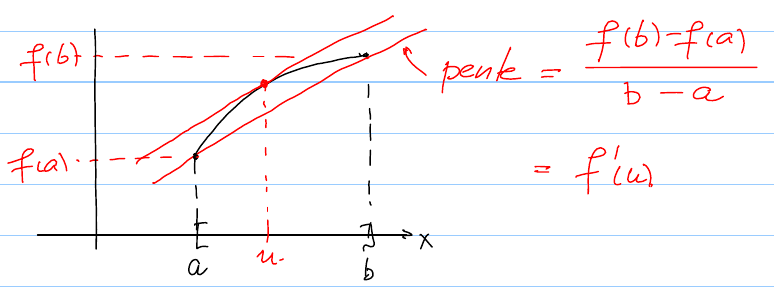
\includegraphics[scale=0.7]{illustrations_Analyse/acc_finis}\\
\evid{Démonstration}\\
Soit $g(x) = f(x) - (f(a) + \frac{f(b)-f(a)}{b-a)}(x-a))$\\
$g(a)=g(b) = 0, $g continue sur [a,b], g dérivable sur ]a,b[\\
Par le théorème de Rolle, $\exists u \in ]a,b[$ tel que g'(u) = 0\\
$g'(u) = f'(u) - \frac{f(b)-f(a)}{b-a} = 0$, donc $f'(u) = \frac{f(b)-f(a)}{b-a}$\\
\begin{boite}
\evid{Corollaire 1} Soit $[a,b] = [x,x+h] \in D(f), \overbrace{h}^{b-a} > 0$, f continue sur [x, x+h] 
et dérivable sur ]x,x+h[- Alors il existe $\vartheta \in ]0,1[$ tel que
\begin{equation}
f(x+h) = f(x) + f'(x + \vartheta h)h
\end{equation}
\end{boite}
\begin{boite}
	\evid{Corollaire 2} Soit $[a,b] \subset D(f), b > a, f$ continue sur $[a,b]$, dérivable sur l'intervalle $]a,b[$. Alors
	\begin{enumerate}[label=\roman*)]
		\item $f'(x) \geq 0$ sur $]a,b[ \to f$ croissant sur $[a,b]$
		\item $f' > 0 $ sur $]a,b[\to f$ strictement croissant sur $[a,b]$
		\item $f'(x) \leq 0$ sur $]a,b[ \to f$ décroissant sur $[a,b]$
		\item $f' < 0 $ sur $]a,b[\to f$ strictement décroissant sur $[a,b]$
	\end{enumerate}
\end{boite}
\begin{boite}
	\evid{Corollaire 3} Soit $[a,b] \subset D(f), b>a, f$ continue sur ${a,b}$, dérivable sur $]a,b[$. Alors $f(a) = 0, f' \geq 0 \to f > 0$ sur $[a,b]$
\end{boite}
\begin{boite}
	\evid{Corollaire 4:} Soit $[a,b] \subset D(f), b>a, f$ continue sur ${a,b}$, dérivable sur $]a,b[$. Alors $f'=0$ sur $]a,b[ \to f$ est constant sur $[a,b]$
\end{boite}
\subsubsection{Exemples}
\begin{enumerate}[label=\roman*)]
	\item Estimer la valeur de $\sin(31\degree) (f(x) = \sin(x))$\\
		$\frac{\pi}{6} < \frac{31}{180}\pi = \frac{\pi}{6} + \frac{\pi}{180} < \frac{\pi}{4}$\\
		$\sin(\frac{\pi}{6} + h) = \underbrace{\sin(\frac{\pi}{6}}_{\frac{1}{2}}) + \cos(\frac{\pi}{6} + \vartheta \frac{\pi}{180})\frac{\pi}{180}$\\
		$g(x) = \cos(x)$ est strictement décroissant sur $[\frac{\pi}{6}, \frac{\pi}{4}]$ car $g'(x) = -\sin(x) < 0$ pour $x \in [\frac{\pi}{6},\frac{\pi}{4}]$\\
		Donc $\frac{1}{2} + \frac{\sqrt{2}}{2}\frac{\pi}{180} \leq \sin(31\degree) \leq \frac{1}{2} + \frac{\sqrt{3}}{2}\frac{\pi}{180}$ 	
		\item Montrer que $f(x) = \cos(x)-1+\frac{1}{2}x^2 \geq 0,\forall x \in \R
$. Puisque f est pair, il suffit de contrôler $x \geq 0$. On a
\begin{equation}
f(0) = \cos(0)-1 = 0 \underbrace{\to}_{coroll. 3}\mbox{ il suffit de montrer }f'(x) \geq 0 \pour x \geq 0
\end{equation}
On $f'(x) = -\sin(x) + x\\
f'(0) = 0 \to $ il suffit de montrer $f''(x) \geq 0$ pour $x \geq 0$\\
On a\\
$f''(x) = -\cos(x) + 1 \geq 9 (\to f'(x)$[trou]
\end{enumerate}
\subsubsection{Théorème des accroissements finis généralisés}
\begin{boite}
	\Theoreme Soit $f:\rtor, g:\rtor [a,b] \subset D(f) \cap D(g), f,g$ continues sur $[a,b]$, dérivables sur $]a,b[, g'(x) \neq 0 \forall x \in ]a,b[$. Alors Il existe $u \in ]a,b[$ tel que 
	\begin{equation}
		\frac{f'(u)}{g'(u)} = \frac{f(b)-f(a)}{g(b)-g(a)}
	\end{equation}
\end{boite}
Pour $g(x) = x$ c'est le théorème des accroissements finis.
\evid{Démonstration}\\
On pose $h(x) = f(x) - \left(f(a)+\frac{f(b)-f(a)}{g(b)-g(a)}(g(x)-g(a))\right)$ puis on utilise le théorème de Rolle.

\subsubsection{Règle de Bernoulli de l'Hospital}
\begin{boite}
	\Theoreme Soit f et g deux fonctions déribales sur $]a,b[ \subset D(f) \cap D(g)$ avec $g'(x) \neq 0 \forall x \in ]a,b[$. Si \framecolorbox{red}{white}{$\llimite{x\to a}{x> a}f(x) = \llimite{x\to a}{x >a} g(x) = 0$} et si\\
	%$\llimite{x\to a}{x >a} \frac{f'(x)}{g'(x)} = l \in \R$\\
	%Alors $\llimite{x\to a}{x >a} \frac{f(x)}{g(x)} = \llimite{x\to a}{x >a} \frac{f'(x)}{g'(x)} = l$
\end{boite}
\begin{boite}
\underline{Remarque} (généralisation, BH) On a le théorème analogue pour $\llimite{x\to b}{x < b}...$ pour le cas $\frac{\pm \infty}{\pm \infty}$ au lieu de $\frac{0}{0}$ et pour a =$-\infty$ ou b $= + \infty$
\end{boite}
\evid{Exemples}
\begin{enumerate}[label = \Roman*)]
	\item $\llimite{x \to 0}{x \neq 0}  {\frac{sin(x)}{x}} = \llimite{x\to 0}{x > 0} {\frac{sin(x)}{x}} = \llimite{x\to 0}{x > 0}{\frac{cos(x)}{1}} = \llimite{x\to 0}{x > 0}{cos(x)} = cos(0) = 1$
	\item 
	\item
	\item $\\limite{x\to 0}{x > 0}{x^x} = \llimite{x\to 0}{x > 0}{e^{x\ln(x)}} \overbrace{=}^{exp continue} e^{\llimite{x\to 0}{x > 0}{x\ln(x)}} = e^0 = 1$
	\item $\limite{\ninf} (1+\frac{2}{n})^n \overset{!}{=}  \limite{x\to \infty} (1+\frac{2}{x})^x = \limite{x\to \infty} e^{x\ln(1+\frac{2}{x})} \overbrace{x}^{exp continue} e^{\limite{x\to \infty}(x\ln(1+\frac{2}{x}))} = e^{\limite{x\to\infty}\frac{\ln(1+\frac{2}{x}}{\frac{1}{x}}} = e^{\limite{x\to\infty} \frac{\frac{1}{1+\frac{2}{x}} \frac{-2}{x^2}}{\frac{-1}{x^2}}} = ???$
	\item \framecolorbox{red}{white}{$\llimite{x\to 0}{x > 0}{\frac{1}{x^p} e^{-\frac{1}{x} = 0}}$} ???
	\begin{enumerate}[label=\roman*.]
		\item 
		\item $0 < p \leq 1$\\
				$\llimite{x\to 0}{x > 0}{\frac{1}{x^p}e^{-\frac{1}{x}}} = \llimite{x\to 0}{x>0}{\frac{\frac{1}{x^p}}{e^{\frac{1}{x}}}} = \llimite{x \to 0}{x>0}{\frac{\frac{-p}{x^{p+1}}}{e^{\frac{2}{x} \frac{-1}{x^2}}}} = \llimite{x\to 0}{x>0}{(p\frac{1}{x^{p-1}} e^{-\frac{1}{x}}} ??? $
				\item ????
	\end{enumerate}
\end{enumerate}

\evid{Bémol :}
Attention !!!!!! La réciproque e BH est fausse !\\
$\llimite{x\to 0}{x > 0}{x \\sin(\frac{2}{x}} \overbrace{=}^{th. des 2 gendarmes} 0\\
0 = \llimite{x\to 0}{x > 0}{x\sin(\frac{1}{x})} = \llimite{x\to 0}{x >0}{\frac{x^2\sin(\frac{1}{x}}{x}} \overbrace{=}^{BH} \llimite{x\to 0}{x > 0}{\frac{2x\sin(\frac{1}{x} - \cos(\frac{1}{x})}{1}}$ n'existe pas.	

\evid{Démonstration de BH}
\begin{enumerate}[label=\roman*)]
	\item f.g continues sur$]a,x[ \subset ]a,b[$ pour tout $a < x<b$
	\item f,g continues sur $[a,x]$ par prolongement continu, si on définit $f(a) = g(a) = 0$.
	\item On a le théorème des accroissements finis généralisé sur $[a,x]$ (si $g'(u) \neq 0 $ pour tout $u \in ]a,x[$)
	\item $\frac{f(x)}{g(x)} = \frac{f(x) - 0}{g(x) - 0} = \frac{f(x)-f(a)}{g(x)-g(a)} \overbrace{=}^{th. des accroissements finis} \frac{f'(u)}{g'(u)} \pour u \in ]a,x[$.\\
	Puisque $u \to a$ lorsque $x\to a$ on a \\
	$\llimite{x\to a}{x > a}{\frac{f(x)}{g(x)}} = \llimite{u \to a}{u > a}{\frac{f'(u=}{g'(u)}}$ \underline{Si cette limite existe !}\\
	\begin{boite}
	Ici on regarde toutes les suites $(u_n$) telles que $u_n  > a, \limite{\ninf}u_n = a$. Mais $u \in ]a,x[$ \underline{Dépend de x} et on ne devrait regarder que les suites ($u_n$) générées par les suites $(x_n$) dans la limite originale.
	\end{boite}
\end{enumerate}
\evid{Démonstration du théorème de la section 5.7}
Rappel : \begin{boite}
	\Theoreme : Soit f:\rtor, $x_0 \in ]a,b[ \subset D(f)$. Soit f continue sur $]a,b[$, et dérivable. $[a,b]\setminus\{x_0\}$ et soit $\llimite{x \to x_0}{c \neq x_0}{f'(x)} = l$\\
	Alors f est dérivable en $x_0$ et $f'(x) 
	= l$
\end{boite}
\evid{Démonstration}
$f'(x_0) \overbrace{=}^{def} \llimite{h \to 0}{x \neq 0}{\frac{f(x_o+h) - f(x_0)}{h}} \overbrace{=}^{BH} \limite{\substack{h\to 0 \\ h > 0 \\ ou \\ h < 0}} \left( \frac{f'(x_0+h}{1'}\right) \overbrace{=}{hypothese} l$
\subsection{Etude des fonctions}
Dans ce chapitre, f: \rtor , I = [a,b]$ \subset D(f), a < b$.
\subsubsection{Définitions}
[dessin courbe étrange]\\
\begin{itemize}
	\item[\evid{Convexe}] f est convexe sur $I_0 si \forall x_1, x_2 \in I_0, x_1 \neq x_2, x_1 < x_2, \lambda x_1 + (1-\lambda)x_2 \in [x_1,x_2]$ pour $\lambda \in [0,1]$-\\
Si $f(\lambda x_1 + (1-\lambda)x_2 \leq \lambda f(x_1) + (1-\lambda) f(x_2)$
\item[\evid{Concave}] f est concave sur $I_0$ si $\forall x_1, x_2, x_1 < x_2\\
f(\lambda x_1 + (1-\lambda)x_2 \geq \lambda f(x_1) + (1-\lambda) f(x_2)$
	\item[\evid{Point critique}] f admet un point critique en $x_0 \in ]a,b[$ si f'($x_0) = 0$
	\item[\evid{Maximum local}] f admet un maximum local en $x_0 \in ]a.b[$ si $f'(x_0) \geq f(x)$ pour x proche de $x_0$ )$\exists \epsilon > 0$ tel que $\forall x$ tels que $|x-x_0 < \epsilon$)
	\item[\evid{Maximum local}] f admet un maximum local en $x_0 \in ]a.b[$ si $f'(x_0) \leq f(x)$ pour x proche de $x_0$ )$\exists \epsilon > 0$ tel que $\forall x$ tels que $|x-x_0 < \epsilon$)
	\item[\evid{Extremum local}] f admet un maximum local ou un minimum local.
	\item[\evid{Maximum local}] f admet un maximum global en $x_0 \in [a,b]$ si $f(x_0) \geq f(x)$ pour tout $x \in [a,b]$.
	\item[\evid{Minimum local local}] f admet un minimum global en $x_0 \in [a,b]$ si $f(x_0) \leq f(x)$ pour tout $x \in [a,b]$.
	\item[\evid{Points d'inflexion}] f admet un point d'inflexion en $x_0 \in ]a,b[$, si f est dérivable en $x_0$ et s'il existe un $\epsilon > 0$ tel que f soit convexe (concave) sur $[x0 -  \epsilon, x_0]$ et concave (convexe) sur $[x_0, x_0 + \epsilon]$
\end{itemize}
\begin{boite}
	\Theoreme (convexe)\\
	Si f' est une fonction croissante sur $I_0$ (en particulier si $f''\geq 0$ sur $I_0$ voir corollaire 2, section 5.10.2) Alors f est convexe sur $I_0$
\end{boite}
\begin{boite}
	\Theoreme (concave)\\
	Si f' est une fonction décroissante sur $I_0$ (en particulier si $f''\leq 0$ sur $I_0$ voir corollaire 2, section 5.10.2) Alors f est concave sur $I_0$
\end{boite}
\evid{Remarque} Toujours avoir en tête les exemples.\\
$f(x) = x^2$ (convexe sur \R)\\
$f(x) = -x^2$ (convexe sur \R)
\begin{boite}
	\Theoreme (extremum local)
	\begin{enumerate}
		\item si f admet un extremum local en $x_0 \in ]a,b[$ et si $f'(x_0)$ existe, alors $f'(x_0) = 0$
		\item f admet un maximum local en $x_0$, si $f'(x_0) = 0$ et $f''(x_0) < 0$
		\item f admet un minimum local en $x_0$, si $f'(x_0) = 0$ et $f''(x_0) > 0$
	\end{enumerate}
\end{boite}
\begin{boite}
\evid{Remarque} (cas général, voir développement limités)
\begin{enumerate}
	\item maximum local si $f'(x_0)=...=f^{(n-1)}(x_0) = 0, f^{(n)}(x_0) < 0$ (n pair)	
	\item maximum local si $f'(x_0)=...=f^{(n-1)}(x_0) = 0, f^{(n)}(x_0) > 0$ (n impair)
\end{enumerate}
\end{boite}
\begin{boite}
	\Theoreme (extremum global)\\
	Soit $f:\rtor [a,b] \subset D(f), f$ continue sur $[a,b]$. Les points $x_0 \in [a,b]$ pour lesquels f admet un extremum global sont éléments de :
	\begin{enumerate}[label=\roman*)]
		\item $\{a,b\}$%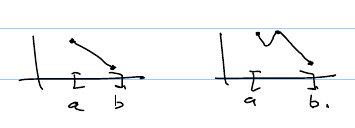
\includegraphics[scale=0.5]{illustrations_analyse/extremum_blobal_ab}
		\item \{des points où f' n'existe pas\}
		\item \{les points ou f' = 0\}
	\end{enumerate}
\end{boite}
\begin{boite}
	\Theoreme (points d'inflexion)\\
	Soit la fonction $f:\rtor$ deux fois dérivables sur $]a,b[ \subset D(f)$
	\begin{enumerate}[label=\roman*)]
		\item si $f$ admet un point d'inflexion en $x_0 \in ]a,b[$, alors $f''(x) = 0$
		\item $f$ admet un point d'inflexion en $x_0 \in ]a,b[$ si $f''(x)$ = 0, si $f'''(x)$ existe et si $f'''(x) \neq 0$
	\end{enumerate}
\end{boite}
\begin{boite}
	\evid{Remarque} (cas général)\\
	$f$ admet un point d'inflexion si $f''(x) = ... = f^{(n-1)} = 0, f^{((n)}\neq 0, n$ impair
\end{boite}
L'exemple a retenir : $x^5, x^7,..$.

\subsubsection{Discuter le graphe d'une fonction}
\begin{enumerate}
	\item Trouver $D(f), \Im (f)$
	\item symétries (paire, impaire, périodique)
	\item zéros de $f$
	\item continuité (limites à gauche et à droite pour les poins de discontinuité de $f$ et les points au bord du domaine)
	\item Dérivabilité de f ("calculer" $f', f'',...$ trouver le domaine  de définition de ces fonctions)
	\item Points particuliers (points critiques, extremums, points ou $f'$ n'existe pas)
	\item monotonie de $f$ (signe de $f'$), convexité/concavité de $f$ (signe de $f''$)
	\item Asymptotes
	\item Tracer le graphe
\end{enumerate}

\subsubsection{Exemples}
[magnifique dessin qui ressemble a une paire de fesses]
\begin{align*}
f(x) &= |2x-1|-x^2+1\text{ sur }[-3,3]\\
	 &=\left\{
	 		\begin{array}{lll}
				2x-x^2 & \pour & x \in [\frac{1}{2},3]\\
				2-2x -x^2 & \pour & x\in [-3,\frac{1}{2}]
			\end{array}
		\right.	
\end{align*}
\begin{enumerate}
	\item  $D(f) = [-3,3], \Im(f) = [m,M]$ à trouver
	\item pas de symétrie
	\item $2x-x^2 = 0$ sur $[\frac{1}{2}, 3], x = 2$\\
	$2-2x-x^2 = 0$ sur $[-3,\frac{1}{2}], x = 1-\sqrt{1+2} = -1-\sqrt{3} £= 2,7...$
	\item $f$ continue sur $[-3,3]$ (composition de fonctions continues)
	\item f dérivable sur $[-3,\frac{1}{2}[ (I_1)$ et sur $[\frac{1}{2},3](I_2)$ (mais $f$ pas dérivable sur $[-3,3]$\\
	\begin{align*}
		\text{Sur } I_1 : & f(x) = -2x-x^2+2\\
		& f'(x) = -2-2x\\
		&f''(x) = -2\\
		I_2 : & f(x) = 2-x^2\\
		& f(x) = 2-2x\\
		& f''(x) -2
	\end{align*}
	\item Points particuliers : $x = \frac{1}{2}, \llimite{x\to\frac{1}{2}}{x > \frac{1}{2}}{f'(x)} = 1 \neq \llimite{x\to\frac{1}{2}}{x<\frac{1}{2}}{f'(x)} = -3$\\
	on a $f(\frac{1}{2}) = \frac{3}{4}$ (minimum local)\\
	Points où $f' = 0$:\\
	 sur $[\frac{1}{2},3], 2-2x = 0, x = 1, f''(1) = -2 \to f$ admet un maximum local : $f(1) = 1$\\
	 sur $[-3,\frac{1}{2}[, -2-2x = 0 x = -1, f''(-1) = -2 \to f$ admet un maximum local en $f(-1) = 3$\\
	 \underline{Maximum et minimum global}\\
	 valeurs aux bords : $f(-3) = -1, f(3) = -3$\\
	 $M = \max\{-1,-3,1,3\} = 3$\\
	 $m=\min\{-1,-3,\frac{3}{4}\} = -3$\\
	 d'où $\Im(f) = [-3,3]$.
	 \item \underline{monotonicité} (tableau des signes)\\
	 $f'(-1) = f'(1) = 0, f'$ pas défini en $x=\frac{1}{2}$
	 \begin{enumerate}[label=\roman*)]
	 	\item sur $[-3,-1], f'(-3) = 4$ et $f''(x) =-2$ sur cet intervalle. $f'$ est donc décroissant  sur [-3,-1] et $0 \leq f'(x) \leq 4$. f est donc croisant sur cet intervalle. 
	 	\item Sur $[-1,\frac{1}{2}] : f'(-1) = 0$ et $f''(x) = -2, f'$ est décroissant sur $[-1,\frac{1}{2}]$ et $-3 \leq f'(x) \leq 0$. $f$ est donc décroissant sur cet intervalle
	 	\item Sur $[\frac{1}{2},1], f'(\frac{1}{2}) = 1$ et $f''(x) = -2, f'$ est décroissant et $0\leq f'(x) \leq 1 \to$ f est donc croissant
	 	\item Sur [1,3] : $f'(1) = 0$ et $f''(x) = -2, f$ est décroissant et $-<\leq f'(x)\leq 0$. f est donc décroissant
	 \end{enumerate}
	 \underline{concavité, convexité} f est concave sur $I_1$ et $I_2$ et f n'a donc aucun point d'inflexion. Attention ! f est concave sur $I_1$ et $I_2$ mais f n'est ni concave ni convexe sur $I = I_1 \cup I_2$
\end{enumerate}

\subsubsection{Exemples avec limites}
(Discussions à compléter!)

\evid{Exemple} $f(x) = \ln(x)$
\begin{boite}[0.5]
 $\llimite{x\to 0}{x > 0}{f(x)} = -\infty$ (tangente verticale)
\end{boite}
\begin{boite}[0.6]
	$\limite{x\to \pm \infty} f(x) = b_{\pm} \in \R$, asymptote horizontal
\end{boite}
exemple $e^x$
\begin{boite}
	\evid{Cas de droites de la forme $y = ax+b$}\\
	$\limite{x\to\pm\infty} \frac{f(x)}{x} = a_{\pm}, \limite{x\to\pm\infty} (f(x)-a_{\pm}x) = b_{\pm}$
\end{boite}
[trou exemple x\^5]

\subsection{Développement en séries et développement limité}
\subsubsection{Définitions}
\begin{boite}
	\evid{Définition} une série de la forme
	\begin{equation}
		s = \somme{\infty}{k=0} \underbrace{a_k (x-a)^k}_{b_k} := \limite{\ninf} \underbrace{\somme{n}{k=0}a_k(x-a)^k}_{s_n}
	\end{equation}
	avec $a\in  \R, a_k \in \R$ (donnés) et $x \in \R$ (un paramètre) est appelé  \textit{une série entière} (à cause des puissances "entières" de (x-a), au lieu de $|x-a|^{\frac{1}{3}k}$ par exemple.
\end{boite}
\begin{itemize}
	\item Le nombre a et les $a_k$ sont considérés comme fixes, et on s'intéresse à la convergence de la série et sa somme en fonction du paramètre x
	\item Souvent on pose $x = a+\xi$ (étude locale proche de x=a). Donc $|\zeta| < r \iff |x-a| < r \iff$ [dessin]
\end{itemize}

\begin{boite}
	\Theoreme Il existe r $\in \R, 0 \leq r \leq \infty$, tel que la série entière 
	\begin{equation}
		s = \somme{\infty}{k=0}{a_x(x-a)^k} = \somme{\infty}{k=0}{a_k\xi^k}
	\end{equation}
	Converge absolument pour $|\xi| < r$ (r dans l'intervalle $]a-r,a+r[$). La série diverge pour $|\xi| > r (x \not \in [a-r,a+r]$)
\end{boite}
\begin{boite}
	\Definition Le nombre r dans le théorème est appelé "rayon de convergence" de la série
\end{boite}

\begin{boite}
	\Theoreme (*) On a \\
	$r = [\limite{k\to\infty}(|a_k|^{\frac{1}{k(]^{-1}}}$ Cauchy\\
	ou $r = \limite{k\to\infty} \left|\frac{a_k}{a_{k+1}}\right|$ D’Alembert\\
	Si ces limites existent
\end{boite}
\evid{Remarques}
\begin{itemize}
	\item Le théorème ne dit rien sur la convergence de la série pour $x = a+r$ et $x=a-r$ (à contrôler séparément)
	\item Si $r = \infty$ (d'Alembert) la série converge pour tout $x\in\R$
	\item Si $r=0$ la série ne converge que pour $x = a$ et $s = a_0$
\end{itemize}
\evid{Remarque} La série converge en fait pour tout $z \in \C$ tel que $|z-a| <r$, c'est à dire pour $z$ dans un disque centré en $a$ de rayon $r$ d'où le nom rayon de convergence.\\
\evid{Démonstration du théorème (*)} $s = \somme{\infty}{k=0}{\underbrace{b_k}_{a_k(x-a)^k}}$\\
%[trou]\\
\underline{Critère de d'Alembert}\\
$q = \limite{k\to\infty} \left|\frac{b_{k+1}}{k_k}\right| = |x-1|\limite{k\to\infty}\left|\frac{a_{k+1}}{a_k}\right| < 1$
[trou]
\subsubsection{Fonctions définies par une série entière}
\begin{boite}
Nouveau point de vue : une série entière définie une fonction (pour $a_1,a_k$ donnés)
\begin{equation}
	f(x) = \somme{\infty}{k=0}{a_x(x-a)^k} (\text{si r $>$ 0})
\end{equation}
et $D(f) \supset ]a-r,a+r[$
\end{boite}
\subsubsection{Dérivée des fonctions définies par une série}
\begin{boite}
	\Theoreme Soit $f(x):= \somme{\infty}{k=0}{a_k(x-a)^k}$ et soit le rayon de converge $r > 0$. Alors
	\begin{equation}
		f'(x) = \somme{\infty}{k=0}{a_{k+1}(k+1)(x-a)^k}
	\end{equation}
\end{boite}
\underline{Explication} On dérive terme par terme dans la série pour \\
$f: \underbrace{\left(\somme{\infty}{k=0}{a_k(x-a)^k}\right)}_{a_0+a_1(x-1)+..)}' = \somme{\infty}{k=1}{a_kk(x-a)^{k-1}}$
[trou]
\begin{boite}
	\Theoreme Soit $f(x):= \somme{\infty}{k=0}{a_k(x-a)^k}$ et soit le rayon de convergence $r > 0$. Alors 
	\begin{equation}
		f^{(n)}(x) = \somme{\infty}{k=0}{a_{k+n}\frac{(k+n)!}{k!}(x-a)^k}
	\end{equation}
	et le rayon de convergence de la série pour $f^{(n)}$ est r.
\end{boite}
\begin{boite}
\underline{Conséquence} Si f est définie par série entière, on a $f^{(n)}(a) = n!a_n$, ou 
\begin{boite}[0.25]
	$a_k = \frac{1}{x!}f^{(k)}(a)$
\end{boite}
\end{boite}
\underline{Notation} Soit I un intervalle ouvert. Alors on note 
\begin{itemize}
	\item $C^{\circ}(I) = \{f:\rtor : I \subset D(f)$, f continue sur I\}
	\item $\underbrace{C^k(I)}_{\mathclap{\substack{\text{des fonctions de} \\ \text{ classe } C^k}}} = \{f:\rtor I\subset D(f), f k$-fois dérivable sur I et $f^{(k)}$ est continue sur i\}
	[trou]
\end{itemize}
\subsubsection{Théorème de Taylor}
\begin{boite}
	\Theoreme (formule de Taylor avec reste, ou développement limité d'ordre n)\\
	Soit f une fonction de classe $C^{n+1}(I)$ pour un $n \in \N$ et soit $a,x \in I$
	\begin{equation}
		f(x) = \underbrace{\somme{n}{k=0}{a_k(x-a)}^k}_{p_n(x)}+R_n(a,x)
	\end{equation}
	avec \fcolorbox{red}{white}{$a_k = \frac{1}{k!}f^{(k)}(a)$}. Alors 
	\begin{center}
		\fcolorbox{red}{white}{$R_n(a,x) = \frac{1}{(n+1)!}f^{(n+1)}(u)(x-a)^{n+1}$}
	\end{center}
	où $u \in ]a,x[$ si $x>a$ et $u\in ]x,a[$ si $x< a$
\end{boite}
\evid{Remarque} Pour n=0 on a $f(x) = f(a) + R_0(a,x)$ avec $R_0(a,x) = f'(u)(x-a)$ ce qui n'est rien d'autre que le théorème des accroissements finis.\\
\evid{Idée de la démonstration}\\
%[trou]\\
\evid{Interprétation géométrique du théorème de Taylor}\\
{graphique}
Pour $f(x) = \sin(x) et a=0$ on trouve\\
$\begin{array}{lllr}
a_0 & = \frac{1}{0!}f(0) & =0 & p_0(x)=0\\
a_1 & = \frac{1}{1!}f'(0) & =1 & p_1(x)=x\\
a_2 & = \frac{1}{2!}f''(0) & =0 & p_2(x)=x\\
a_3 & = \frac{1}{3!}f'''(0) & =-\frac{1}{6} & p_3(x)=x\\
\end{array}$
\subsubsection{Développement d'une fonction en une série}
\evid{Remarque} Si f  est de classe $C^\infty(I)$ on peut utiliser la formule d Taylor avec reste pour n arbitraire (mais à priori $n \leq \infty$).
\begin{boite}
	\Theoreme (série de Taylor)\\
	Si f est de classe $C^\infty(I)$ et si \fcolorbox{red}{white}{$\limite{\ninf}R_n(a,x) = 0$} on obtient à partir du théorème de Taylor avec reste (pour x fixe)
	\begin{equation}
	f(x) = \somme{\infty}{k=0}{a_x(x-a)^k} \text{ (série de taylor)}
	\end{equation}
	et si a=0
	\begin{equation}
		fx) = \somme{\infty}{k=0}{a_kx^k} \text{ (Série de Mac Laurin)}
	\end{equation}
	{trou}
\end{boite}
Donc (formule de Taylor)
\begin{equation}
	f(x) = \somme{n}{k=0}{\underbrace{1}_{a_k} x^k + R_n(x)}
\end{equation}
avec
\begin{equation}
	R_n(x) = \frac{1}{(n+1)!}f^{(n+1)}(n)x^{n+1} = \frac{1}{(1-u)^{n+2}}x^{n+1} = \frac{1}{1-u}\left(\frac{x}{1-u}\right)^{n+1}
\end{equation}
avec $u \in ]0,x[$ si $x>0$ et $u \in]x,0[$ si $x<0$\\
Puisque $x\in I = ]-\frac{1}{4}, \frac{1}{4}$[
{trou}\\
En fait on a cette égalité pour $x \in ]-1,1[$ mais pas dans $D(f) = \R\setminus\{1\}$
\evid{Contre exemple}
\underline{remarque} la condition $f \in C^\infty(I)$ n'est pas suffisant pour que f puisse être développé en une série entière\\
Soit $f(x) = \left\{\begin{array}{lll}
e^{-\frac{1}{x}} & \pour & x>0\\
0 & \pour & x<0
\end{array}\right.$
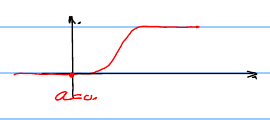
\includegraphics[scale=0.5]{illustrations_analyse/e_1_sur_x_2}\\
On a \begin{itemize}
	\item $\llimite{x\to 0}{x>0}{f(x)} = 0 = f(0) \to f$ continue sur \R
	\item $f'(x) = \frac{1}{x^2}e^{-\frac{1}{x}} \pour x >0$\\
	$f'(x) = 0 \pour x \leq 0$\\
	$\llimite{x\to 0}{x>0}{f'(x)} = 0 = f'(0)$ (voir le théorème chapitre 5.7 pour cette égalité)
	\item Par récurrence, on montre que $D(f^k) = \R$ et que $f^{(k)}(0) = 0$\\
\end{itemize}
Donc $f\in C^\infty(\R)$ et $f^{(k)}(0) = 0, k = 0,1,2,...$\\
\underline{Formule de Taylor avec reste en x = a = 0}
\begin{boite}[0.25]
$a_k = \frac{1}{k!}f^{(k)}(0) = 0$
\end{boite}
\begin{itemize}
	\item $x < 0 : f(x) = 0 = \underbrace{\somme{n}{k=0}{a_kx^k}}_{=0} + R_n(x)\\
	\to \R_n(x) = 0, n = 0,1,2,...$
	\item $x > 0 : f(x) = e^{-\frac{1}{x}} = \underbrace{\somme{n}{k=0}{a_kx^k}}_{=0} +R_n(x)\\
	\to R_n(x) = e^{-\frac{1}{x}}$
\end{itemize}
Donc pour $x > 0 \limite{\ninf}R_n(x) = e^{-\frac{1}{x}} (=f(x)$
\begin{boite}
Conclusion : $f\in C^\infty(\R)$ mais f$\not\in C^{\omega}(\R)$ car f ne peut pas être représenté proche de x=0 par une série entière.
\end{boite}

\subsubsection{Les fonctions $\exp, \sinh, \cosh, \sin, \cos, \ln, (1-x)^\alpha$}
\evid{Développement limité de $e^x$}\\
Soit $I=\R, a=0,$ et $f(x) = e^x, f^{(n)}(x) = e^x$ et $f^{(n)}(0) = 1$
\begin{equation}
	e^x = \somme{n}{k=0}{\frac{1}{k!}x^k} + \underbrace{\frac{1}{(n+1)!}e^ux^{n+1}}_{=R_n(x), |u| < |x|}
\end{equation}
\evid{Développement de $e^x$ en une série entière}\\
On a $|R_n(0,x)| \leq \underbrace{^{|x|} \frac{|x|^{n+1}}{(n+1)!}}_{\ninf = 0}, \forall x \in \R$\\
et donc
\begin{boite}
$e^x = \somme{\infty}{k=0}{\frac{1}{k!}x^k}, \forall x \in \R$
\end{boite}
$r = \limite{k\to\infty}\frac{\frac{1}{k!}}{\frac{1}{(x+1)!}} = \limite{k\to\infty}(k+1) = \infty$
\evid{Les fonctions $\sinh$ et $\cosh$}\\
Avec la même procédure :
\begin{boite}
\begin{equation}
\sinh (x) = \somme{\infty}{k=0}{\frac{1}{(2k+1)!}x^{2k+1}}
\end{equation}
\begin{equation}
\cosh( x) = \somme{\infty}{k=0}{\frac{1}{(2k)!}x^{2k}}
\end{equation}
\end{boite}
\evid{Les fonction $\sin, \cos$}\\
Avec la même procédure\\
\begin{boite}
	\begin{equation}	
		\sin(x) = \somme{\infty}{k=0}{\frac{(-1)^k}{(2k+1)!}x^{2k+1}}
	\end{equation}
	\begin{equation}
		\cos(x) = \somme{\infty}{k=0}{\frac{(-1)^k}{(2k)!}x^{2k}}
	\end{equation}
\end{boite}
\evid{La fonction $\ln(1+x)$}\\
\includegraphics[scale=0.5]{illustrations_Analyse/ln_1_x}\\
$\ln(1+x) = \somme{\infty}{k=1}{\frac{(-1)^{k+1}}{k}x^k}$, $x\in ],1,1[$\\
\underline{Démonstration}\\
$\underbrace{\frac{d}{dx}\ln(1+x)}_{=\frac{1}{1+x}} = \somme{\infty}{k=1}{\frac{(-1)^{k+1}}{k}\cdot k\cdot x} =
 \somme{\infty}{k-1=l, l=0}{(-1)^lx^l} = \somme{\infty}{l=0}{(-x)^l}= \frac{1}{1-(-x)} = \frac{1}{1+x}$
\evid{La fonction $(1+x)^\alpha, \alpha\in\R$}\\
On a $\frac{1}{n!}\frac{d^n}{dx^n} (1+x)^\alpha = \frac{1}{n!}\alpha(\alpha-1)...(\alpha-n+1) = \combi{\alpha}{n}$
\begin{boite}
	\begin{equation}
		(1+x)^\alpha = \somme{\infty}{k=0}{\combi{\alpha}{n}x^n}, \forall x \in ]-,1[
	\end{equation}
\end{boite}
\evid{Fonction exponentielle complexe et formule d'Euler}\\
Démonstration de la formule d'Euler :\\
On définit l'exponentielle $\exp(z) = \somme{\infty}{k=0}{\frac{1}{k!}z^k}$\\
$\exp(ix)= \somme{\infty}{k=0}{\frac{1}{k!}i^kx^k} = \underbrace{\somme{\infty}{k=0}{\frac{(-1)^k}{(2k)!}x^{2k}}}_{\cos(x)} + i\cdot \underbrace{\somme{\infty}{k=0}{\frac{(-1)^k}{(2k+1)!}x^{2k+1}}}_{\sin(x)} = \cos(x) + i \sin(x)$
\subsubsection{La notation o et O}
\begin{boite}
	\Definition Soit $n \in \N$. On écrit que $f(x) = o((x-a)^n), x\to a$\\
	si 
	\begin{equation}
		\llimite{x\to a}{x\neq a}{\frac{f(x)}{(x-a)^n}} = 0
	\end{equation}
\end{boite}
et on écrit que $f(x) = O((x-a)^n), x\to a$\\
Si
 \begin{equation}
	\left|\frac{f(x)}{(x-a)^n}\right| < C \in \R \text{ Proche de x=a, x$\neq$a}
\end{equation}
\evid{Remarque} Cas n=0 : $f(x) = o(1), x\to a$ veut dire
\begin{equation}
	 \limite{x\to a}\frac{f(x)}{1}=0
\end{equation}
\evid{Remarque} Si $f(x) =o(x^n), x\to 0$, alors $cf(x) = o(x^n), x\to 0$
\evid{Remarque} Si $f(x) = o(/x-a)^n), x\to a$
\begin{equation}
	\frac{f(x)}{(x-a)^m} = o((x-a)^{n-m}) x\to a
\end{equation}
$0 <m < n, m,n \in \N$\\
Pour le développement limité d'une fonction en $x=a$, on a avec cette notation:
\begin{boite}
$\begin{array}{ll}
	f(x) &= p_n(x)+R_n(a,x) \\
	&= p_n(x)+o((x-a)^n), x\to a
\end{array}$
\end{boite}
Car $\frac{R_n(a,x)}{(x-a)^n} = \frac{1}{(n+1)!}\underbrace{f^{(n+1)}(u)}_{=f^{(n+1)}(a)}(x-a) \substack{\to\\ x\to a\\ x\neq a} 0$
\evid{Exemples :}\\
\begin{itemize}
	\item $\frac{1}{1-x} = 1+\underbrace{x+x^2 + x^3 + o(x^3)}_{o(x)} = 1+o(1)$
	\item ---
	\item $e^x=1+x+\frac{1}{2!}x^2 + \frac{1}{3!}x^3+o(x^3)$
	\item $\sin(x) = x-\frac{1}{3!}x^3 +\frac{1}{5!}x^5 + o(x^5)$
	\item $\cos(x) = 1-\frac{1}{2!}x^2+\frac{1}{4!x^4+o(x_4)}$
	\item $\ln(1+x) = x-\frac{1}{2}x^2 + \frac{1}{3}x^3-\frac{1}{4}x^4+o(x^4)$
	\item $\ln(x) = \ln(1+\underbrace{(x-1)}_{X \to 0 (x\to 1))}) = ...$
\end{itemize}
\evid{Exemples de limites}
$\llimite{x\to 0}{x\neq 0}{\frac{\sin(x)}{x}}=\llimite{x\to 0}{x\neq 0}{\frac{x+o(x)}{x}}=\llimite{x\to 0}{x\neq 0}{(1+o(1)} = 1$\\
$\llimite{x\to 0}{x\neq 0}{\frac{1-\cos(x)}{x^2}} = \llimite{x\to 0}{x\neq 0}{\frac{1-(1-\frac{1}{2}x^2+o(x^2))}{x^2}} = \llimite{x\to 0}{x\neq 0}{\frac{1}{2}+o(1)} = \frac{1}{2}$
\evid{Composition de développement limités}\\
\begin{enumerate}
	\item $\frac{1}{\cos(x)} = \frac{1}{(1+\underbrace{(\cos(x)-1)}_{X}}$\\
	$X = \frac{-1}{2}x^2 + \underbrace{\frac{1}{24}x^4 + o(x^4)}_{o(x^2}$, donc $x\substack{\longrightarrow \\ x\to 0} 0$\\
	$\frac{1}{(1+X} = 1-X+X^2+o(X^2)$\\
	$\frac{1}{\cos(x)} = 1-(\frac{-1}{2}x^2 + \frac{1}{24}x^4 + o(x^4)) +(-\frac{1}{2}x^2+\underbrace{\frac{1}{24}x^4+o(x^4))}_{0(x^2)}^2+o(x^4)$\\
	$=1+\frac{1}{2}x^2 - \frac{1}{24}x^4 + o(x^4) + \frac{1}{4}x^4 + o(x^4)\\
	 = 1+\frac{1}{2}x^2 + \frac{5}{24}x^4 + o(x^4)$
	 \item $\tan(x) = \frac{\sin(x)}{\cos(x)} = \sin(x) \frac{1}{\cos(x)}, x\to 0$\\
	 $=(x-\frac{1}{6}x^3 + o(x^3))\cdot(1+\frac{1}{2}x^2 + o(x^2)\\
	 =x+\frac{1}{2}x^3 -\frac{1}{6}x^3 + o(x^3)\\
	 =x+\frac{1}{3}x^3 + o(x^3)$
	 \item $f(x) = \sin(\tan(x))-\tan(\sin(x))$\\
	 $\sin(x) = x-\frac{1}{3!}x^3 +\frac{1}{5!}x^5 + o(x^5)\\
	 \cos(x) = 1-\frac{1}{2!}x^2+\frac{1}{4!x^4+o(x_4)}$\\
	 $=x+\frac{1}{3}x^3 + o(x^3)-\frac{1}{6}(x+o(x))^3\\
	 -(x-\frac{1}{6}x^3+o(x^3) + \frac{1}{3}(x+o(x))^3$\\
	 $=x+\frac{1}{3}x^3 - \frac{1}{6}x^3 - x + \frac{1}{6} x^3 - \frac{1}{3}x^3+o(x^3)\\
	 = o(x^3)$\\
	 En fait (vérifier !)\\
	 $f(x) = -\frac{1}{30}x^7 + o(x^7)$
\end{enumerate}


\section{Intégrales indéfinies et définies}
\setcounter{equation}{0}
\subsection{Définition de l'intégrale indéfinie}
$\eth =$ dérivée\\
$\eth: C^1(]a,b[) \to C^0(]a,b[)$ ($C^1:$ les fonctions dérivées une fois, et qui sont encore continues sur la fonction dérivée) (pas injectif)\\
$f: \to D(f) = f'$ (surjectif). Il s'agit de la fonction dérivée.\\
attention, $f+c$ arrive aussi sur f'. c est une constante. \\
$\eth^{-1} : C^1(]a,b[ \leftarrow C^0(]a,b[)$\\
$\eth^{-1}(f) \leftarrow f$\\
$\eth^{-1}(f= : \{F \in C^1(]a,b[) : F' = f\}$

\begin{boite}
	\Definition Soit $f\in C^0(]a,b[)$. Une primitive de f est une fonction $F \in C^1(]a,b[)$ telle que $F'(x) = f(x)$ pour $x \in ]a,b[$
\end{boite}
\Remarque F est dérivable sur $[a,b]$ car F' = f et continue sur $[a,b]$ (voir le théorème de la section 5.7)\\
\Remarque Deux primitives d'une fonction ne diffèrent que d'une constante.
\begin{boite}
\Definition On appelle intégrale indéfinie de f l'ensemble des primitives de f.
\end{boite}
\evid{Notation} $F(x) = \int f(x)dx$ ou \textcolor{red}{$\int^x f(t) dt$}.\\
\evid{Exemples :}\\
$\begin{array}{lll}
f & F & \text{Domaine de Définition}\\
\hline
x^n & \frac{1}{n+1}x^{n+1} + C & n\neq 1, C \in \R (n \in \R\setminus\{-1\}\\
\frac{1}{x}& \ln(|x|) + c & x \in \R^* \\
\cos(x) & \sin(x) + C &\\
\sin(x) & -\cos(x) + C &\\
e^x & e^x + c &\\
\ln(x) & x\cdot\ln(x) - x + C & x > 0\\
\tan(x) = \frac{\sin(x)}{\cos(x)} & -\ln(|\cos(x)|) + C & x \in D(\tan(x)\\
\frac{f'(x)}{f(x)} & \ln(|f(x)|) +C\\
\frac{1}{1+x^2} & \arctan(x) + C &\\
\frac{f'(x)}{1+f(x)^2} & \arctan(f(x)) + C &\\
e^{x^2} 2x & e^{x^2} &\\
nx^{n-1}+2x{n+1}e^{x^2} & x^ne^{x^2} + C
\end{array}$\\
\Remarque\\
L'application  $\eth : C^1 (]a,b[) \to C^0 (]a,b[)$ est Linéaire : $\eth(\alpha f + \beta g) = \alpha\eth(f) +  \beta\eth(g), \alpha \beta \in \R, f,g \in C^1 (]a,b[). \eth^{-1}$ est aussi linéaire.
\begin{equation}
 \int(\alpha f(x) + \beta g(x))dx = \alpha \int f(x)dx + \beta\int f(x) dx	
\end{equation}
\subsection{Définition de l'intégrale définie}
Soit f une fonction continue de \rtor $[a,b]\subset D(f), a\leq b$\\
\begin{center}
\includegraphics[scale=0.8]{illustrations_analyse/integrale}
\end{center}
\begin{boite}
	\Definition Soit $n \in \N^*$. alors une suite $(x_n), a \equiv x_0 \leq x_1 \leq x_2 ... \leq x_n \equiv b$ est appelée une partition de [a,b]
\end{boite}
\evid{Notation} On écrira $\wp (x_0,x_1,....x_n)$ pour une partition d'une intervalle $[a,b]$
\begin{boite}
	Soit $n \in \N^3, \wp(x_o,...x_n)$ une partition de $[a,b], u_i \in [x_{i_1},x_i], i = 1,\ldots,n$. Alors on appelle
	\begin{equation}
		S_n = \somme{n}{i=1}{f(u_i)(x_i-x_{i-1})}
	\end{equation}	 
	La somme de Riemann de f pour la partition $\wp(x_0,\ldots, x_n)$ et le choix de $(u_i)_{i=1,\ldots,n}$
\end{boite}
\Remarque Si $f \leq 0$ sur $[a,b]$, alors la somme de Riemann est une approximation de la ``surface sous le graph de f ''.\\
\Remarque Puisque la fonction f est continue sur $[a,b]$ on a 
\begin{equation}
	m\cdot(b-a) \leq S_n \leq M(b-a)
\end{equation}
où m et M dont le minimum et le maximum global de f sur $[a,b]$.\\
\Remarque Puisque f est continue sur $[a,b]$, f est continue sur $[x_{i-1},x_i]$ et f admet un minimum $m_i$ et un maximum $M_i$ sur $[x_{i-1},x_i]$ et \\
$(b-a)m \leq \underline{S_n} \leq S_n \leq \overline{S_n} \leq (b-a)M$, ou :
\begin{itemize}
	\item $\underline{S_n} = \somme{n}{i=1}{m_i(x_1-x_{i-1})}$
\end{itemize}
\begin{boite}
	\Definition Soit $n \in \N^*$. Donnée une partition $\wp(x_0,\ldots x_n)$, on définit $\Delta x \equiv \Delta x (\wp) := \max\{x_1-x_0. x_2-x_1,...\}$ la taille de la partition.
\end{boite}
\evid{Exemple} (découpage régulier).\\
On définit
\begin{center}$
x_i = a + \frac{b-a}{n}i, i=0,1,\ldots n$
\end{center}
\begin{center}$
	\Delta x = \frac{b-a}{n}
$\end{center}


\begin{boite}
\evid{Définition / Théorème (intégrale définie de f sur [a,b])}\\
	Soit f une fonction contiunue sur [a,b] $\wp_n \equiv \wp (x_0,\ldots,x_m), n\in \N^*$ une suite de partitions telles que $\limite{\ninf}{\Delta x (\wp_n)} = 0$. Alors es $\limite{\ninf}{\underline{S}} = \limite{\ninf}{\underline{S}}$ et $\overline{S} = \limite{\ninf}{\overline{S}}$ existent, sont indépendants du choix des la suite des partitions et $\underline{S} = \overline{S} =: S$. Le nombre S est apelé "intégrale définie de f sur [a,b]
\end{boite}
\evid{Explication de $\underline{S} = \overline{S}$}\\
La continuité de f sur [a,b] implique$^{(*)}$ que $\forall \epsilon > 0$, il existe $n_0$ tel que $\forall n \geq n_0. |M_i -m_i| < \frac{\epsilon}{b-a}, i 0 1,...,n$, c'est à dire $|\overline{S} - \underline{S}| \leq \epsilon$

\evid{Limite épointée} {trou}\\
\evid{continuité en $x \in D(f)$} {trou}
\evid{Notation} on écrit $\int_a^b f(x) dx$ pour l'intégrale définie sur $[a,b]$ 

{trou}

\subsection{Propriétés de l'intégrale définie}

\begin{boite}
	\begin{enumerate}
		\item linéarité
		{trou}
	\end{enumerate}
\end{boite}
\subsection{Théorème de la moyenne}
\includegraphics[scale=0.5]{illustrations_analyse/theo_moyenne}\\
\begin{boite}
\Theoreme Soit $f: \rtor [a,b] \subset D(f), b>a, f$ continue sur $[a,b]$. Alors il existe $u \in ]a,b[$ tel que 
\begin{equation}
\int_a^b f(x) dx = f(u)(b-a)
\end{equation}
\end{boite}
\evid{Remarque} $f(u) = \frac{1}{b-a}\int_a^bf(x) \, \mathrm dx$ = valeur moyenne de f sur $[a,b]$.\\
\underline{Démonstration :} Théorème des accroissements finis (donné le théorème fondamental du calcul intégral).\\
\begin{boite}
	\evid{Théorème généralisé}\\
	Soit $f,g \rtor, [a,b] \subset D(f) \cap D(g), f,g$ continues sur $[a,b], g(x) > 0, \forall x \in [a,b]$. Alors il existe $u \in]a,b[$ tel que
	\begin{equation}
		\int_a^b f(x) \cdot g(x) \, \mathrm{d}x = f(u) \cdot \int_a^bg(x) \, \mathrm dx
	\end{equation}	 
\end{boite}
Pour $g(x) = 1$ c'est le théorème précédent
\underline{Démonstration} Théorème ds accroissements finis généralisé  + théorème fondamental du calcul intégral.
\subsection{Théorème fondamental du calcul intégral}
\begin{boite}
	\Theoreme Soit$f:\rtor, [a,b] \subset D(f), f$ continue sur [a,b], alors
	\begin{enumerate}
		\item La fonction G définie par $G(x) = \int_a^b f(t) dt$ est une primitive de f sur ]a,b[, c'est à dire G est dérivable sur ]a,b[ et G'(x) = f(x).
		\item Si F est une primitive de f sur ]a,b[,alors 
		\begin{equation}
			\int_a^b f(x) dx = F(b) - F(a)
		\end{equation}
			\end{enumerate}
\end{boite}
\begin{enumerate}[label = \roman*)]
	 \item Soit $x \in ]a,b[$ alors
$
	 	\frac{G(x+h) - G(x)}{h} = \frac{1}{h}\left(\intt{a}{x+h}{f(t)} - \intt{a}{x}{f(t)}\right) = \\
	 	\frac{1}{h}\intt{x}{x+h}{f(t)} \underbrace{=}_{\mathclap{\substack{\text{par le théorème de la}\\ \text{avec g(x) = 1}}}} \frac{1}{x} f(u) h = f(u)
$
	 pour $u \in ]x,x+h[, h > 0$ et $u \in ]x+h,x[, h < 0$\\
	 Donc $ u \to x$ lorsque $h \to 0$ et $f(u) \to f(x)$ car f est une fonction continue sur $[x,x+h] ([x+h,x])$
	 \item Soit F une primitive de f. Alors il existe $C \in \R$ tel que
	 \begin{equation}
	 	F(x) = G(x) + C \text{ POur tout x} \in [a,b]
	 \end{equation}
	 Pour x = a on a $F(a) = 0+C = C$\\
	 Donc $F(x) = G(x) + F(a)$ et on trouve \\
	 $F(b) = \underbrace{G(b)}_{=\intx{a}{b}{f(x)}} + F(a)$\\
	 D'où $\intx{a}{b}{f(x)} = F(b) - F(a)$
\end{enumerate} 
\evid{Remarque} Pour f continue sur ]a,b[ la fonction $G(x) = \intt{c}{x}{f(t)}$ est une primitive de f pour tout choix de $c \in ]a,b[$. L'application $\eth : C^1(]a,b[) \to C^0(]a,b[)$ est donc surjective.\\
\evid{Notation} On écrira\\
$\intx{a}{b}{f(x)} = \left[F(x)\right]_a^b \equiv F(b) - F(a)$\\
\evid{Exemples}\\
\begin{enumerate}[label=\arabic*)]
	\item $\intx{0}{1}{1} = \left[x\right]_0^1 = 1-0 = 1$
	\item $\intx{0}{2\pi}{\sin(x)} = \left[-\cos(x)\right]_0^{2\pi} = -1-(-1) = 0$
\end{enumerate}
\newpage
\subsection*{Résumé du Théorème fondamental du calcul Intégral}
\begin{boite}
	\Definition Soit $f \in C^0 ([a,b])$. Une primitive de f est une fonction $F \in C^1(]a,b[)$ telle que $F'(x) = f(x)$ pour tout $x \in ]a,b[$
\end{boite}
\evid{Remarque} F est dérivable sur [a,b] (voir le théorème section 5,7) \textcolor{red}{et F est donc continue sur [a,b]}
\begin{boite}
	\Definition Soit $f \in C^0)[a,b])$. La limite $S := \underline{S} = \overline{S}$ où $\overline{S} = \limite{\ninf}\overline{S_n}, \underline{S} = \limite{\ninf}\underline{S_n}$ est appelé intégrale définie de f sur [a,b]
\end{boite}
\evid{Notation}\\
$\int_a^b f(x) dx \in \R\to$ intégrale définie\\
$\int f(x) dx \equiv \int^x f(t)dt\to$ intégrale indéfinie = $\{F \in C^1(]a,b[) : F' = f\}$\\
\includegraphics[scale=0.5]{illustrations_analyse/notation_integrale}\\
on montre que $\llimite{x\to a}{x>a}{G(x)} = 0 =: G(a)$
\begin{boite}
	\Theoreme Soit $f \in C^0 ([a,b])$. Alors 
	\begin{enumerate}[label=\roman*)]
		\item G est une primitive de f
		\item $\int_a^b f(x)\, \mathrm dx = F(b) - F(a)$\\
		pour toute primitive F de f
	\end{enumerate}
\end{boite}
\begin{boite}
\evid{Théorème de la moyenne}\\
soit $f\in C^0([a,b]), g\in C^0([a,b]), g(x) > 0$ pour tout $x \in [a,b]$, Alors il existe $u \in ]a,b[$ tel que
\begin{equation}
	\intx{a}{b}{f(x)g(x)} = f(u)\intx{a}{b}{g(x)}
\end{equation}
\end{boite}
\evid{Démonstration}
Soient m et M le minimum et le maximum global de f sur [a,b]. Alors $m\cdot g(x) \leq f(x)g(x) \leq Mg(x)$ et donc
\begin{equation}
	m\intx{a}{b}{g(x)} \leq \intx{a}{b}{f(x)g(x)} \leq M\intx{a}{b}{g(x)}
\end{equation}
et il existe donc $v \in [m,M]$ tel que 
\begin{equation}
	\intx{a}{b}{f(x)g(x)} = v\intx{a}{b}{g(x)}
\end{equation}
Par le théorème de la valeur intermédiaire, il existe $u \in]a,b[$ tel que $v = f(u)$
\newpage
\subsection{Application du théorème de la moyenne}
\evid{Proposition :} $\frac{2}{7	} \leq \underbrace{\intx{0}{\pi}{\frac{\sin(x)}{5+\sqrt[3]{x}}}}_I \leq \frac{2}{5}$\\
\evid{Démonstration} On a $\sin(x) > 0$ pour $x \in ]0,\pi[$. On pose \\
$f(x) = \frac{1}{5+\sqrt[3]{x}}, g(x) = \sin(x)$\\
$\exists u \in ]0,\pi[$ tel que \\
$I= f(u) \cdot \underbrace{\intx{0}{\pi}{\sin(x)}}_{= [-\cos(x)]_0^\pi = 1+1 = 2}$\\
f est une fonction décroissante sur $[0,\pi]$ et $f(0) = \frac{1}{5}, f(\pi) = \frac{1}{5+\sqrt[3]{\pi}} > \frac{1}{7}$\\
Donc $\frac{2}{7} \leq I \leq \frac{2}{5}$
\subsection{Méthode d'intégration}
\subsubsection{Intégration "immédiate"}
\underline{Voir le tableau}
\begin{enumerate}
	\item $a > 0, \int a^x \, \mathrm dx = \int e^{x\ln(a)}  \, \mathrm dx = \frac{1}{\ln(a)}e^{x\ln(a)} + C = a^x\frac{1}{\ln(a)} + C$
	\item $\int f(x)\cdot f'(x)  \, \mathrm dx = \frac{1}{2}f(x)^2 + C$\\
	\underline{Exemple :} $\int \sin(x)\cos(x)  \, \mathrm dx = \frac{1}{2} \sin(x)^2 + C = -\frac{1}{2}\cos(x)^2 + C$ (à cause de la constante)
	\item $\int \frac{f'(x)}{f(x)} \, \mathrm dx = \ln(|f(x)|) + C$\\
	\underline{Exemple :} $\int \tan(x)  \, \mathrm dx = -\int \frac{-\sin(x)}{\cos(x)} \, \mathrm dx = -\ln(|\cos(x)|) + C$
	\item $\intx{0}{\frac{\pi}{2}}{\sin(x)^2} = \intx{0}{\frac{\pi}{2}}{\frac{1}{2}(1-cos(2x)} = [\frac{x}{2}-\frac{1}{4}\sin(2x)]_0^\frac{\pi}{2} = \frac{\pi}{4}$
	\item $\intx{0}{n\cdot\frac{\pi}{2}}{\sin(x)^2} = n \cdot \frac{\pi}{4}$ (on fait n fois la même aire)
\end{enumerate}\
\subsubsection{Intégration par changement de variable}
\begin{boite}
	\Theoreme soit $f:\rtor, [a,b] \subset D(f), f$ continue sur $[a,b]$. Soit $\varphi : [\alpha,\beta]\to[a,b], \varphi$ dérivable sur $[\alpha,\beta]$, et et $\varphi'$ continue sur $[\alpha,\beta]$. De plus :\\
	\fcolorbox{red}{white}{$\varphi(\alpha) = a, \varphi(\beta) = b$}\\
	\includegraphics[scale=0.8]{illustrations_analyse/integ_partie}\\
	Alors \fcolorbox{red}{white}{$\intx{a}{b}{f(x)} = \int_{\alpha}^{\beta}f(\varphi(u)) \cdot \varphi'(u)  \, \mathrm du$}
\end{boite}
\evid{Démonstration}\\
Soit F une primitive de f sur [a,b], alors la fonction$F : G(u) = F(\varphi(u))$ est une primitive de $f(\varphi(u)) \cdot \varphi'(u)$ sur $[\alpha,\beta]$, car
\begin{equation}
	G'(u) = F'(\varphi(u)) \cdot \varphi'(u) = f(\varphi(u)) \cdot \varphi'(u)
\end{equation}
En plus $\int_\alpha^\beta f(\varphi(u)) \cdot \varphi'(u) \, \mathrm du = [G(u)]_\alpha^\beta = G(\beta)-G(\alpha)$\\
$ = F(\varphi(\beta)) - F(\varphi(\alpha)) = F(b) -F(a) = \intx{a}{b}{f(x)}$\\
 \evid{Remarque :} Si $\varphi$ est bijective, alors $F(x) = G(\varphi^{-1}(x))$

\evid{Exemples :}
\begin{enumerate}
	\item $I = \intx{0}{1}{\sqrt{1-x^2}} = \frac{\pi}{4}$. On pose $x =\varphi(u) = \sin(u); \varphi : [0,\frac{\pi}{2}] \to [0,1]$\\
	$I = \int_0^{\frac{\pi}{2}} \underbrace{\sqrt{1-\sin^2(u)}}_{|\cos(u)|} \cdot \underbrace{\cos(u)}_{\varphi'(u)} \, \mathrm du$\\
	$= \int_0^{\frac{\pi}{2}} \cos^2(u) \, \mathrm du = \int_0^{\frac{\pi}{2}} (1-\sin^2(u)) \, \mathrm du = \frac{\pi}{2} - \int_0^\frac{\pi}{2} \sin^2(x) \, \mathrm du = \frac{\pi}{4}$
	\item Cas d'une intégrale indéfinie (voir la remarque)\\
	$F(x) = \int \sqrt{1-x^2} \, \mathrm dx $\\
	$x = \varphi(u) = \sin(x), \varphi : [0,\frac{\pi}{2}] \to [0,1]$\\
	$G(u) = \int (1-\sin^2(u) \, \mathrm du = u-(\frac{1}{2}u - \frac{1}{4}\sin(2u)) = \frac{1}{2}u + \frac{1}{4}\underbrace{\sin(2u)}_{=2\sin(u)\cos(u)}$\\
	$= \frac{1}{2}u + \frac{1}{2} \sin(u)\sqrt{1-\sin^2(u)}$\\
	Donc F(x) = $G(\varphi^{-1}(x)) =  = G(\arcsin(x)) = \frac{1}{2}\arcsin(x) + \frac{1}{2}x\sqrt{1-x^2}$
\end{enumerate}
\subsubsection{Intégration par partie}
\begin{boite}
	\Theoreme Soit $f: [a,b] \to \R, g : [a,b] \to R$ continûment dérivable sur $[a,b]$ (= dérivable avec une fonction dérivée qui est continue). Alors 
	\begin{equation}
		\intx{a}{b}{f'(x)g(x)} = [f(x)g(x)]_a^b - \intx{a}{b}{f(x)g'(x)}
	\end{equation}

\evid{Remarque}\\
En pratique, on écrit l'identité plutôt comme \\
\begin{equation}
	\intx{a}{b}{f(x)g(x)} = [F(x)g(x)]_a^b - \intx{a}{b}{F(x)g'(x)}
\end{equation}
Avec f continue sur [a,b] et g continûment dérivable sur [a,b].\\
\evid{Remarque} (cas d'une intégrale indéfinie)\\
\begin{equation}
	\int f(x)g(x) \, \mathrm dx = F(x)g(x) - \int F(x) g'(x) \, \mathrm dx
\end{equation}
f continue, g continûment dérivable, F une primitive de F.
\end{boite}
\evid{Démonstration}\\
\begin{equation}
(f\cdot g)'(x) = f'(x)g(x) + f(x)g'(x)
\end{equation}
et donc 
\begin{equation}
	\intx{a}{b}{(f\cdot g)'} = \intx{a}{b}{f'(x)g(x)} + \intx{a}{b}{f(x)g'(x)}
\end{equation}
\evid{Exemples}
\begin{enumerate}
	\item $\intx{0}{1}{e^xx} = [e^xx]_0^1-\intx{0}{1}{e^x1}$
	\item $\intx{0}{1}{x^2e^x} = [e^xx^2]_0^1 - \underbrace{\intx{0}{1}{e^x(2x)}}_{2\intx{0}{1}{e^xx}}$
	\item $\intx{}{}{\ln(x)} = x\ln(x) - \int{}{}{\underbrace{x\frac{1}{x}}_{=1}} = x\ln(x) - x + C$ 
	\item $\intx{0}{\frac{\pi}{2}}{\sin(x)^n} = I_n, I_0 = \frac{\pi}{2}, I_1 = 1, n \in \N^*$\\
	$n\geq 2 : I_n = \intx{0}{\frac{\pi}{2}}{\sin(x)\sin(x)^{n-1}}\\ 
	= [-\cos(x)\sin(x)^{n-1}]_0^{\frac{\pi}{2}} + \intx{0}{\frac{\pi}{2}}{\cos(x)(n-1)(\sin(x)^{n-2}\cos(x)} \\
	= (n-1)\intx{0}{\frac{\pi}{2}}{\sin(x)^{n-2}(1-\sin(x)^2)} \\
	= (n-1)I_{n-2} - (n-1)I_n$\\
	Donc $nI_n = (n-1)I_{n-2}$ ou \framecolorbox{red}{white}{$I_n = \frac{n-1}{n}I_{n-2}$}\\
	Donc $I_2 = \frac{1}{2}I_0 = \frac{\pi}{4}$
	\item $\intx{}{}{\frac{1}{(x^2+1)^n}} = I_n, I_0 = x+C, I_1 = \arctan(x) + C$.\\
	$n\geq 1 : I_n = \intx{}{}{1\cdot\frac{1}{(x^211)^n}}\\
	= x\frac{1}{(x^2+1)^n} + 2n \intx{}{}{\underbrace{x \frac{1}{(x^2+1)^{n+1}} x}_{= \frac{(x^2+1)-1}{(x^2+1)^{n+1}}}}\\
	I_n = \frac{x}{(x^2+1)^n} + 2n I_n - 2nI_{n+1}$\\
	Donc $I_{n+1} = \frac{1}{2n} \frac{x}{(x^2+1)^n}+\frac{2n-1}{2n} I_n, n = 1,2,3....$\\
	$\to I_2 = \frac{1}{2} \frac{x}{x^2+1} + \frac{1}{2}\arctan(x) + C$
	\end{enumerate}
\subsection{Intégration d'un développement limité}
\begin{boite}
\evid{Proposition :} Soit
\begin{equation}
	f(x) = f(a) + f'(a)(x-a) + \ldots + \frac{1}{n!}f^{(n)})a=(x-a)^n + \o((x-a)^n)
\end{equation}
lorsque $x\to a$ Alors :\\
$F(x) := \int_a^x f(x) \, \mathrm dt \\
= f(a)(x-a) + \frac{f'(a)}{2}(x-a)^2 + \ldots +\frac{1}{(n+1)!}f^{(n)}(a) (x-a)^{n+1} + o((x-a)^n)$\\
lorsque $x\to a$
\end{boite}
\evid{Démonstration}
Soit $x > a, g$ continue sur $[x,a], \llimite{x\to a}{x>a}{\frac{g(x)}{(x-a)^n}} = 0$\\
$\int_a^x g(t) \, \mathrm dt \underbrace{=}_{\mathclap{\substack{\text{theoreme de}\\\text{la moyenne}}}} g(u)(x-a)$ avec $u \in ]a,x[$\\
Donc $\left| \frac{\int_a^xg(t)\, \mathrm dt}{(x-a)^{n+1}}\right| = [trou...]$\\
Idem pour $x<a$\\
\evid{Exemples}\\
Soit $F(x) := \intt{0}{x}{\sin(\cos(x))}$. calculer le $DL_5$ (développement limité d'ordre 5) de F en x = 0. ON a besoin du $DL_4$ de $f(t) = \sin(\cos(t))$ en t = 0.
\begin{enumerate}[label=\roman*)]
	\item $\cos(t) = 1- \underbrace{ \frac{1}{2}t^2 + \frac{1}{24} t^4 + o(t^4)}_{=T\mbox{ et }T \to 0 \pour t \to 0}$
	\item il nous faut le développement limité de sin en x=1 (car cos(0) = 1). Il suffit de calculer le $DL_2$ de sin(x) en x=1 (car $T \equiv t^2$)\\
	$\sin(x) = \sin(1) + \cos(1)(x-1) - \frac{1}{2}\sin(1)(x-1)^2 + o((x-1)^2)$\\
	$\sin(\cos(t)) = \sin(1+T) = \sin(1)+\cos(1)T - \frac{1}{2}\sin(1)T^2 + o(T^2)$
	\item $f(t) = \sin(1) +  \cos(1)(\frac{1}{2}t^2 + \frac{1}{24}t^4 + o(t^4)) - \frac{1}{2}\sin(1)(-\frac{1}{2}t^2 + o(t^2))^2 + o(t^4)$\\
	$f(t) =  \sin(1) - \frac{1}{2} \cos(1)t^2 + (\frac{1}{24}\cos(1) - \frac{1}{8} \sin(1))t^4 + o(t^4)$
	\item $F(x) = \sin(1)x - \frac{1}{6} \cos(1)x^3$
\end{enumerate}
\subsection{Intégration d'une série entière}
\begin{boite}
	\Theoreme Une Série entière peut être intégrée terme par terme. Soit 
	\begin{equation}
		f(x) = \somme{k=0}{\infty}{a_k(x-a)^k}
	\end{equation}
	avec rayon de convergence $r > 0$. Alors 
	\begin{equation}
		F(x) := \intt{a}{x}{f(t)} = \somme{k=0}{\infty}{a_k \frac{1}{k+1}(x-a)^{k+1}}
	\end{equation}
	avec rayon de convergence r.
\end{boite}
\evid{Démonstration :} $F(a) = 0, F'(x) = f(x)$\\
\evid{Exemple:}\\
Soit $f(x) = \frac{2}{\sqrt{\pi}}e^{-x^2}$. \fcolorbox{red}{white}{$e^x = \somme{k=0}{\infty}{\frac{1}{k!}x^k}$}\\
Donc $f(x) =  \frac{2}{\sqrt{\pi}} \somme{k=0}{\infty}{\frac{1}{k! (-1)^k x^{2k}}}$\\
%[deux dessins]\\
Alors $erf(x) := \intt{0}{x}{f(t)} = \frac{2}{\sqrt{\pi}} \somme{k=0}{\infty}{\frac{1}{k!} \frac{1}{2k+1} (-1)^k x^{2k+1}}$\\
\subsection{Intégrales généralisées (ou impropres)}
$I = \intx{a}{b}{f(x)}$, trois types :
\begin{enumerate}
	\item \evid{Type 1 :}\\
		f continue sur $[a,b[$, ou $]a,b]$, ou $]a,b[$
		[image]
	\item \evid{Type 2 :}\\
	f continue sur $]-\infty,b], [a, \infty[, ]-\infty,\infty[$ ($a = -\infty, b = \infty$, ou les deux)
	[image]
	\item \evid{Type 3 :}\\
	Combinaison des types 1 et 2.
\end{enumerate}
\evid{Exemples explicites :}\\
\includegraphics[scale=0.5]{Illustrations_Analyse/ex_explicites2}\\
\begin{boite}
	\Definition (type 1)\\
	\begin{itemize}
		\item Si f est continue sur $]a,b]$
		\begin{equation}
			\intx{a}{b}{f(x)} := \llimite{\epsilon \to 0}{\epsilon  \neq 0}{\intx{a+\epsilon}{b}{f(x)}}
		\end{equation}
		\item Si f est continue sur $[a,b[$
		\begin{equation}
			\intx{a}{b}{f(x)} := \llimite{\epsilon \to 0}{\epsilon  \neq 0}{\intx{a}{b-\epsilon}{f(x)}}
		\end{equation}
		\item Si f est continue sur $]a,b[$
		\begin{equation}
			\intx{a}{b}{f(x)} :=\limite{\substack{\epsilon_1 \to 0 \\ \epsilon_1 > 0 \\ \epsilon_2 \to 0 \\ \epsilon_2 > 0}}\intx{a+\epsilon}{b-\epsilon}{f(x)}
		\end{equation}
		(une limite après l'autre, l'ordre ne joue pas d'ordre).
	\end{itemize}
\end{boite}
\evid{Exemples}
\begin{enumerate}
	\item $\intx{0}{1}{\ln(x)} \overbrace{=}^{def} \llimite{\epsilon \to 0}{\epsilon > 0}{\intx{\epsilon}{1}{1\ln(x)}}$\\
	$= \llimite{\epsilon \to 0}{\epsilon > 0}{([x\ln(x)]_\epsilon^1 - \intx{\epsilon}{1}{1})}$ {trou}
	\item {trou}
	\item 
\end{enumerate}
\begin{boite}
	\Definition (type 2)\\
	\begin{itemize}
		\item Si f est continue sur$[a,\infty[$
		\begin{equation}
			\intx{a}{\infty}{f(x)} := \limite{R \to \infty}\intx{a}{R}{f(x)}
		\end{equation}
		\item Si f est conitnue sur $]-\infty,b]$
		\begin{equation}
			\intx{-\infty}{b}{f(x)} := \limite{R \to \infty}\intx{R}{b}{f(x)}
		\end{equation}
		\item Si f est continue sur $]-\infty,\infty[$
		\begin{equation}
			\intx{-\infty}{\infty}{f(x)} = \llimite{R_2 \to \infty}{R_1 \to -\infty}{\intx{R_1}{R_2}{f(x)}}
		\end{equation}
		De nouveau, n'importe quel ordre.
	\end{itemize}
\end{boite}
\evid{Exemples}:
\begin{enumerate}
	\item $\intx{0}{\infty}{e^{-x}} = \limite{R \to \infty}\intx{0}{R}{e^{-x}}$\\
	$= \limite{R\to \infty}[-e^{-x}]_0^R = \limite{R\to \infty}(-e^{-R} + 1) = 1$
	\item {trou}
	\item $r \neq 1, r > 0 \intx{1}{\infty}{\frac{1}{x^r}} = \limite{R \to \infty}\intx{1}{R}{\frac{1}{x^r}} = \limite{R \to \infty} [\frac{1}{1-r} \frac{1}{x^{r-1}}]_1^R \\
	= \limite{R\to\infty}\left(\frac{1}{1-r}\frac{1}{R^{r-1}} - \frac{1}{1-r}\right) = \left\{
	\begin{array}{ll}
	+\infty & r < 1\\
	\frac{1}{r-1} & r > 1
	\end{array}\right.$\\
	cas r = 1 : $ \intx{1}{\infty}{\frac{1}{x}} = \limite{R \to \infty} \intx{1}{R}{\frac{1}{x}}\\
	 = \limite{R \to \infty}[\ln(x)]_1^R = \limite{R \to \infty}(\ln(R) - 0) = +\infty$
	 \begin{boite}
	 	\evid{Définition : (type 3)}\\
	 	Si f est continue sur $]a,\infty[$ ou $]-\infty,b[$ :
	 	\begin{equation}
	 		\intx{a}{\infty}{f(x)} := \intx{a}{c}{f(x)} + \intx{c}{\infty}{f(x)}\text{ avec } c \in ]a,\infty[
	 	\end{equation}
	 	\begin{equation}
	 		\intx{\infty}{b}{f(x)} := \intx{-\infty}{c}{f(x)} + \intx{c}{b}{f(x)} \text{ avec } c \in ]-\infty,b[
	 	\end{equation}
	 \end{boite}
\end{enumerate} 
\begin{boite}
\evid{Remarque :}\\
$\intx{a}{\infty}{f(x)} = \limite{\substack{R \to \infty \\ \epsilon \to 0 \\ \epsilon > 0}} \intx{a+\epsilon}{R}{f(x)}$\\
$\intx{-\infty}{b}{f(x)} = \limite{\substack{R \to -\infty \\ \epsilon \to 0 \\ \epsilon > 0}}
\intx{R}{b-\epsilon}{f(x)}$
\end{boite}
\evid{Exemple : }\\
$\intx{0}{\infty}{\frac{1}{\sqrt{x}}e^{-x}} = \limite{\substack{R \to \infty \\ \epsilon \to 0 \\ \epsilon > 0}} \intx{\epsilon}{R}{\frac{1}{\sqrt{x}} e^{-x}} =: I$. Pour se débarrasser de la racine, on pose $x = \varphi(u)= u^2, u > 0, \varphi(\sqrt{\epsilon}) = \epsilon, \varphi(\sqrt{R}) = R$\\
$I = \limite{\substack{R \to \infty \\ \epsilon \to 0 \\ \epsilon > 0}} \int_{\sqrt{\epsilon}}^{\sqrt{R}} \frac{1}{u}e^{-u^2}\cdot 2u \, \mathrm du$ (on se rappelle que $erf(x) = \frac{2}{\sqrt{\pi}} \int_0^x e^{-u^2} \, \mathrm du$)\\
$= \limite{\substack{R \to \infty \\ \epsilon \to 0 \\ \epsilon > 0}} [\sqrt{\pi}erf(x)]_{\sqrt{\epsilon}}^{\sqrt{R}]}\\
= \limite{\substack{R \to \infty \\ \epsilon \to 0 \\ \epsilon > 0}} (\sqrt{\pi} erf(\sqrt{R} - \sqrt{\pi}erf(\sqrt{\epsilon}) = \sqrt{\pi}$

\subsection{Intégration des foncitons rationnelles}
Soit $f(x) = \frac{p(x)}{q(x)}$ avec p,q des polynpmee, de gré de p {trou}\\
\\
\evid{Exemple :} $ \frac{x^3+1}{x^2+1} = x + \frac{-x+1}{x^2+1}$\\
Soit donc degré p $<$ degré de q.

\subsubsection{Exemple}
\begin{enumerate}
	\item Décomposition de q(x) (sur \R) en facteur irréductibles.\\
	 \underline{Exemple :} \begin{align*}
	 x^2-1 = (x-1)(x+1)\\
	 x^2+1 = x^2+1 \text{ pas de factorisation sur les reels}\\
	 x^3-1 = (x-1)(x^2+x+1)\\
	 x^3+1 = (x+1)(x^2-x+1)\\
	 x^4-1 = (x^2+1)(x^2-1) = (x^2+1)(x-1)(x+1)\\
	 x^4+1 =  (x^2+\sqrt{2}x + 1)(x^2-\sqrt{2}x +1) \text{voir le chapitre des nombres complexes)}
	 \end{align*}
	 \item Décomposition de $f(x) = \frac{p(x)}{q(x)}$ en éléments simples\\
	 \underline{Exemple :} $f(x) = \frac{2x^3}{x^4-1} = \frac{\alpha}{x-1} + \frac{\beta}{x-1} + \frac{\gamma x + \delta}{x^2+1}$\\
	 $2x^3 = \alpha(x+1)(x^2+1) + \beta(x-1)(x^2+1) + (\gamma x + \delta)(x^2-1)$\\
	 On regarde les coefficients de chaque puissance : \\
	 $\left.
		 \begin{array}{ll}
			 x^3 : & 2 = \alpha + \beta + \gamma\\
			 x^2 : & 0 = \alpha - \beta + \delta\\
			 x : & 0 = \alpha + \beta - \gamma\\
			 1 : & 0 = \alpha - \beta - \gamma
		 \end{array}
		\right\}$ algèbre linéaire : $\alpha = \beta = \frac{1}{2}, \gamma = 1, \delta = 0$
	\item Intégration des éléments simples\\
	$\intx{}{}{f(x)} = \frac{1}{2}\intx{}{}{\frac{1}{x-1}} + \frac{1}{2}\intx{}{}{\frac{1}{x+1}} + \frac{1}{2}\intx{}{}{\frac{2x}{x^2+1}}$\\
	$= \frac{1}{2}\ln(|x-1|) + \frac{1}{2}\ln(|x+1|) = \frac{1}{2}\ln(|x^2+1|) + C\\
	= \frac{1}{2}(\ln(|(x-1)(x+1)(x^2+1)|)) + C\\
	= \frac{1}{2}\ln(|x^4-1|) + C = \ln(\sqrt{x^4 -1}) + C$
	En fait (ouvrir les yeux):\\
	$f8x) = \frac{1}{2} \frac{g'(x)}{g(x)}$ avec $g(x) = x^4-1$\\
	Donc $\intx{}{}{f(x)} = \frac{1}{2}${trou}
\end{enumerate}
\subsubsection{Le cas général}
Soit $f(x) = \frac{p(x)}{q(x)}, \deg p < \deg q$
\begin{enumerate}
	\item Décomposition de q(x) en facteurs irreductibles \\
	$q(x) = (\ldots)(\ldots)(\ldots)...$
	\item Décomposition en éléments simples \\
	\includegraphics[scale=0.5]{Illustrations_Analyse/elements_simples}\\
	Remettre sur le même dénominateur, comparer les puissances, utiliser algèbre linéaire pour déterminerles coefficients $\alpha,\beta,\gamma$
	\item Intégration des éléments simples.
	\begin{itemize}
		\item $\intx{}{}{\frac{1}{x-a}} = \ln(|x-a|) + C$
		\item $intx{}{}{\frac{1}{(x-a)^k}} = -\frac{1}{k-1}\frac{1}{(x-a)^k} + C$, k$\geq 2$
		\item $\intx{}{}{\frac{\beta x + \gamma}{x^2+bx+c}} = \intx{}{}{\frac{\frac{\beta}{2}(2x+b)+\gamma - \frac{1}{2}\beta b}{x^2+bx +c}} \\
		= \frac{\beta}{2} \ln(|x^2+bx+c|) + (\gamma+ \frac{1}{2}\beta b)\intx{}{}{\underbrace{\frac{1}{x^2+bx+c}}_{=(x+\frac{b}{2})^2+c+\frac{b^2}{4}}}$\\
		On a $c - \frac{b^2}{4} > 0$ sinon on aurait des facteurs linéaires !\\
		On pose $x = \varphi(u) = \sqrt{x-\frac{b^2}{4}}u - \frac{b}{2}$\\
		$\intx{}{}{\frac{1}{x^2+bx+c}} = \frac{1}{\sqrt{c+\frac{b^2}{4}}}\int{\frac{1}{u^2+1}} \, \mathrm du$\\
		$= \frac{\beta}{2}\ln(|x^2+bx+c|) + \frac{\gamma\frac{1}{2}\beta b}{\sqrt{c-\frac{b^2}{4}}} \arctan (\frac{x+\frac{b}{2}}{\sqrt{c-\frac{b^2}{4}}} + C$\\
		Finalement, pour $k \geq 2$\\
		$\int\frac{\beta x + \gamma}{(x^2+bx+x)^k} = $ même procédure que pour k = 1	\\
		{trou}
	\end{itemize}
\end{enumerate}
\subsection{Divers}
$\intt{1}{3}{\frac{1}{\sqrt{t}(1+t)}}$. \\
On pose $t = \varphi(s) = s^2$, avec $ s > 0$\\
$1 = \varphi(1), 3 = \varphi(\sqrt{3})$\\
Donc notre :$\intt{1}{3}{\frac{1}{\sqrt{t}(1+t)}} = \int_1^{\sqrt{3}} \frac{1}{s(1+s^2} 2s \, \mathrm ds =  2[\arctan(s)]_1^{\sqrt{3}} = 2(\arctan(\sqrt{3}) - \arctan(1)) = 2(\frac{\pi}{3}-\frac{\pi}{4})$ (voir dessins) = $\frac{\pi}{12}2= \frac{\pi}{6}$\\
\\
Cas indéfini : $\intt{}{}{\frac{1}{\sqrt{t}(1+t)}} = 2 \arctan(s) + C = 2\arctan(\sqrt{t}) + C$








\subsection{Glossaire} 
\begin{itemize}
\item[$\sim$] Relation d'équivalence
\item[:=] est défini par
\item[$\equiv$] Équivalent à
\item[$\forall$] Pour tout (x par exemple)
\item[$\in$] est élément de
\item[$C_x$] Classe d'équivalence de x
\item[:] tel que
\end{itemize}

\subsection{Règles}
\subsubsection{Complexes}
\subsubsection{Limites}
\begin{itemize}
\item $\limite{\ninf} \frac{\sin(n)}{n} = 1$
\item $\limite{\ninf} n\cdot\sin(\frac{1}{n}) = 1$
\item $\limite{\ninf} (1+\frac{1}{n})^n = e$
\end{itemize}
\subsection{Fonctions}
\begin{itemize}
	\item $g(x) = |x| \to g'(x) = 
	\left\{
		\begin{array}{ll}
		-1 & x < 0\\
		1 & x > 0
		\end{array}\right.$ et pas dérivable en x = 0
	\item dérivée de la fonction réciproque donnée par $(f^{-1})'(x) = \frac{1}{f'(f^{-1}(x))}$
	\item $\cos(x) = \sqrt{1-\sin(x)^2}$
\end{itemize}
\end{document}